% !TEX root = ../main.tex

\chapter{Nested Estimation}
\label{chp:nest}

\todo[inline]{Voting probprog example?}

We present a formalization of nested Monte Carlo (NMC) estimation, whereby
terms in an outer estimator are themselves the output of separate, nested, Monte Carlo (MC) estimators.
We demonstrate that NMC can provide consistent estimates of 
nested expectations, including cases of repeated nesting, under mild conditions;
establish corresponding rates of convergence;
and provide empirical evidence that suggests these rates are observed in practice.
We further establish a number of pitfalls that can arise from na\"{i}ve nesting of MC estimators
and provide guidelines about how they can be avoided.
Our results show that whenever an outer estimator depends nonlinearly on an inner
estimator, then the number of samples used in \emph{both} the inner and outer estimators
must, in general, be driven to infinity for convergence.  
We also lay out novel methods for reformulating certain classes of nested expectation problems
into a single expectation, leading to improved convergence rates compared with na\"{i}ve NMC.

%\vspace{-10pt}

% !TEX root =  main.tex

\section{Background}
\label{sec:intro}

%Although interesting alternatives have recently been suggested \cite{briol2015probabilistic}, \mc integration is almost exclusively used to calculate the expectation, given the generated samples.
%the method used in practise for calculating these expectations, given the generated samples, is almost exclusively \mc integration.  
%The calculation of expectations using \mc can be considered intertwined with that of \mc inference.  
%After all, convergence rates that are often quoted for \mc inference schemes, actually correspond to the convergence of the final \mc integration estimate.

There are various problems involving nested expectations that require the use of nested
estimation schemes such as NMC. For example, the expected information gain used in
Bayesian experimental design requires
the calculation of an entropy of a marginal distribution (see Chapter~\ref{chp:design}), and therefore includes the
expectation of the logarithm of an expectation.  By extension, any Kullback-Leibler
divergence where one of the terms is a marginal distribution also involves a nested expectation.  Hence, our results have important implications for relaxing mean field assumptions in variational
inference and deep generative models
\citep{burda2015importance,hoffman2015stochastic,maaloe2016auxiliary,naesseth2017variational,maddison2017filtering,
	le2017auto,rainforth2018tighter}.
%Here the nonlinearity provided by the logarithm prevents a simple reformulation to a
%single expectation in the general case, and thus presents conventional \mc estimation.
Another common nested estimation scenario is calculating expectations with respect to so-called
doubly-intractable distributions~\citep{moller2006efficient,murray2006mcmc,liang2010double}, whereby
the target distribution is only known up to a parameter-dependent normalizing constant.  Here
the normalization constant itself represents an intractable expectation
nested within the overall expectation.
NMC can also arise in contexts demanding the use
of direct \mc simulations, for example in portfolio risk management
\citep{gordy2010nested} and stochastic control \citep{belomestny2010regression}. 
In particular, 
simulations of agents that reason about decisions of other agents or which
reason about sequential decision making processes tend to include nested expectations.
Thus problems like planning in games and ``theory-of-mind'' type meta-reasoning
tend to require some form of nested
 estimation~\citep{stuhlmuller2014reasoning,evans2017models}.

Certain nested estimation problems can be tackled by so-called pseudo-marginal methods
\citep{beaumont2003estimation,andrieu2009pseudo,andrieu2010particle,
	andrieu2015convergence,naessethLS2015nested}.
These consider cases of Bayesian inference where the likelihood is intractable, 
%such as
%when it originates from an Approximate Bayesian Computation (ABC)
%\citep{csillery2010approximate}, 
but can be estimated unbiasedly.
% or when sequential Monte Carlo \cite{smith2013sequential} is used to approximate a high
% dimensional distribution.  
From a theoretical perspective, they involve reformulating the problem in an extended space with auxiliary variables that
are used to represent the stochasticity in the likelihood computation. This then enables the
problem to be expressed as a single expectation.
Our work goes beyond this by also considering cases in which a non-linear mapping is
applied to the output of the inner expectation (such as the logarithm in the 
experimental design case or the inverse for general doubly-intractable distributions), so that 
this reformulation to a single expectation is no longer possible.

NMC with non-linear mappings of the inner expectation has been previously considered in
the financial statistics literature, for example in the pricing of American
options \citep{longstaff2001valuing}. Though most of this literature focuses on
particular application-specific non-linear mappings \citep{broadie2011efficient,gordy2010nested},
convergence bounds for a more general class of models
has been shown by \citet{hong2009estimating}.
We build on these results and outline the opportunities and pitfalls of nesting Monte Carlo
estimators in a machine learning context.
Our proofs apply to a more general class of problems than existing approaches.
For example, we provide the first convergence bounds for cases of multiple levels of estimator nesting
as might occur in a probabilistic programming system.
We further lay out novel methods for reformulating certain classes of nested expectation problems
into a single expectation, allowing the use of conventional \mc estimation 
schemes with superior convergence rates than the na\"{i}ve use of NMC, one of which we
exploit in Chapter~\ref{chp:design} to derive an improved estimator for discrete
Bayesian experimental design problems.
Meanwhile, we provide theoretical results showing that any \mc
estimator using imperfect nested estimates is, in general, biased.  Finally, we provide numerical
experiments, corroborating our theoretical results.

%\tom{Policy search?}

%We now arrive at the crux of this paper: we aim to establish in what nested inference scenarios one can guarentee convergence; we demonstrate that even when a general purpose scheme convergences, it must be biased; and we provide upper bounds on the convergence rate that such a scheme can achieve, showing that it decreases exponentially with the depth of nesting.


% !TEX root =  main.tex

\section{Problem Formulation}
\label{sec:prob-form}

The key idea of MC is that the expectation of an arbitrary function 
$\lambda \colon \mathcal{Y} \rightarrow \mathcal{F} \subseteq \real$ under a probability distribution $p(y)$ for its input $y \in \mathcal{Y}$ can be approximately calculated using:
\begin{align}
\label{eq:MC}
I &= \mathbb{E}_{p(y)} \left[\lambda(y)\right]
\approx \frac{1}{N} \sum_{n=1}^{N} \lambda(y_n) \quad \text{where} \quad y_n \iid p(y).
\end{align}
In this paper, we consider the case that $\lambda$ is itself intractable, defined only in terms of a functional mapping of an expectation. Specifically, $\lambda(y) = f(y,\gamma(y))$
where we can evaluate $f \colon \mathcal{Y} \times \Phi \rightarrow \mathcal{F}$ exactly for a given $y$ and $\gamma (y)$, but $\gamma(y)$ is the output of the following 
intractable expectation of another variable $z \in \mathcal{Z}$:
\begin{subequations}
	\label{eq:gamma}
	\begin{align}
	\label{eq:gamma_1}
	\text{either}\quad
	\gamma(y) &=  \mathbb{E}_{p(z | y)} \left[\phi(y,z)\right] \\
	\label{eq:gamma_2}
	\text{or} \quad \gamma(y) &= \mathbb{E}_{p(z)} \left[\phi(y,z)\right]
	\end{align}
\end{subequations}
depending on the problem, with $\phi \colon \mathcal{Y} \times \mathcal{Z} \rightarrow \Phi \subseteq \real^{D_{\phi}}$.
All our results apply to both cases, but we will focus on~\eqref{eq:gamma_1} for clarity.
Estimating $I$ involves computing two integrals, one for $y$ and the other for $z$. 
We call the approach of tackling both integrations using Monte Carlo 
as \emph{nested Monte Carlo} (NMC):
\begin{subequations}
\label{eq:nested-mc}
\begin{align}
I \approx I_{N,M} &= \frac{1}{N}  \sum_{n=1}^{N} f(y_n,(\hat{\gamma}_M)_n) \label{eq:nested-outer} \quad \;\;  \text{ where } \;\; y_n \iid p(y) \;\;  \text{and} \\
(\hat{\gamma}_M)_n &= \frac{1}{M}  \sum_{m=1}^{M}  \phi(y_n,z_{n,m}) \label{eq:nested-inner} \quad
\text{ where each } \;\; z_{n,m} \sim p(z | y_n) \;\; \text{independently }.
\end{align}
\end{subequations}
In Section~\ref{sec:convergence} we will build on this further by considering cases with multiple
levels of nesting, where computing $\phi(y,z)$ requires the computation of an intractable (nested) expectation.
%Note that for the experimental design example given in~\eqref{eq:exp-design},
%$f(y,\gamma(y)) = \log \gamma(y)$, $\gamma(y)$ is of the form~\eqref{eq:gamma_2}, and
%$\phi(y,z)$ is the likelihood function  $p(y|z,x)$.

The rest of this Chapter proceeds as follows. In Section~\ref{sec:special_cases}, we consider
special cases that allow recovery of the standard MC convergence rate.
In Section~\ref{sec:convergence}, we establish convergence results for $I_{N,M}$ given a
general class of $f$ and extend this to cases of repeated nesting. In Section~\ref{sec:bias}, we establish results demonstrating the
inevitable bias of most possible general-purpose NMC schemes. In Section~\ref{sec:empirical}, 
we present empirical results demonstrating the applicability of NMC and suggesting that our theoretical 
convergence rates are observed in practice.  Longer proofs are provided at the end of the Chapter
in Section~\ref{sec:nest:proofs}.

% !TEX root =  ../main.tex

\section{Special Cases}
\label{sec:special_cases}

We begin by discussing some special cases where it is possible to achieve a
convergence rate of $O(1/N)$ in the mean square error (MSE) as per conventional
MC estimation \citep{robert2004monte}.  
Establishing these cases is important because it identifies what problems we can use existing results for,
when we can achieve an improved convergence rate, and what precautions we must take to ensure this.
The first case is that the top-level integrand $f$ in our estimation problem is linear. 
Section~\ref{sec:linear_case} summarizes the well-known result in this case, which forms the basis for pseudo-marginal, 
nested sequential MC \citep{andersson2015nested}, and ABC methods. The next is that $y$ has finite possible realisations.
The result for this case is given in Section~\ref{sec:discrete}. Though intuitively straight-forward, it 
requires significant care to prove. The third case in Section~\ref{sec:products} is concerned with the product of expectations.
Our result for this case is, to the best of our knowledge, new and applies to many latent variable models and a number 
of probabilistic program examples, e.g. when the probability of a program trace
is weighted by marginal likelihood estimates from other programs.
The last case is that the integrand $f$ is a polynomial (Section~\ref{sec:polynomial}). It 
covers cases such as moment estimation and opens up interesting possibilities in using tractable 
approximations to the integrand $f$.

\subsection{Linear $f$}
\label{sec:linear_case}

Suppose that $f$ 
is integrable and linear in its second argument, i.e. $f(y,\alpha v + \beta w) = 
\alpha f(y,v)+ \beta f(y,w)$.
%or equivalently $f(y,v) = g(y)v$ where
%$g(y)$ can be calculated without an approximate integration.
In this case, we can rearrange the problem to a single expectation:
\begin{align*}
I
& = \mathbb{E}_{y \sim p(y)}\left[f(y,\gamma(y))\right] = \mathbb{E}_{y \sim p(y)}\left[f\left(y,\mathbb{E}_{z\sim p(z|y)}\left[\phi(y,z)\right]\right)\right]
\\
& = \mathbb{E}_{y \sim p(y)}\left[ \mathbb{E}_{z\sim p(z|y)}\left[f(y,\phi(y,z))\right]\right]
 \approx\frac{1}{N} \sum_{n=1}^{N} f(y_n,\phi(y_n,z_n))
\end{align*}
where $(y_n, z_n) \sim p(y)p(z|y)$.
Note that if $\gamma(y)$ is of the form of~\eqref{eq:gamma_2} instead of~\eqref{eq:gamma_1}, then $y$ and $z$ are drawn independently from their marginals instead of the joint.
% or the use of nested queries \cite{goodman2008church,rainforth2016nips} in probabilistic
% programming when the outer query does not depend on any nonlinear functional mapping of
% the marginal probability from the inner query.  
%In these scenarios, nesting provides a convenient means of expressing the problem, but is
%not a fundamental component of its solution.

%Another important case occurs when $\gamma(y)$ is independent of $y$. \todo{Isn't this
%just saying $\gamma$ is constant?}  In this case, we can estimate $\tilde{\gamma} =
%\gamma(y)$ and $(I(f) \,|\, \tilde{\gamma})$ separately, each converging at
%$O(1/\sqrt{N})$, presuming that the same number of samples $N$ is used for both. Provided
%that $f(y,v)$ is Lipschitz continuous in $v$, the root mean squared error of the
%estimation for $I(f)$ will also have same convergence rate.
%\footnote{The proof for this
%follows the same lines as used to link the error in $\gamma$ to $f$ in
%Theorem~\ref{the:Consistent}.} \todo{Do we want this footnote?}

% !TEX root =  ../main.tex

\subsection{Finite Possible Realizations of $y$}
\label{sec:discrete}

If $y$ must take one of finitely many values $y_1, \cdots, y_C$, then it is possible to
use another approach to ensure the same convergence rate as standard MC.
The key observation is to note that in this case we can convert the nested problem
\eqref{eq:MC} into $C$ separate non-nested problems
\begin{align}
         I = \sum_{c=1}^C P(y = y_c) \, f(y_c, \gamma(y_c))
\end{align}
which can then be estimated using
\begin{align}
        I_N  &= \sum_{c=1}^C (\hat{P}_N)_c \, (\hat{f}_N)_c \quad \text{where}
        \label{eq:IN} \\
        \label{eq:PN}
        P(y = y_c) &\approx (\hat{P}_N)_c = \frac{1}{N} \sum_{n=1}^N \mathbbm{1}(y_n = y_c)  \\
        \label{eq:fn}
        f(y_c, \gamma(y_c)) &\approx (\hat{f}_N)_c = f\left(y_c, \frac{1}{N} \sum_{n=1}^N \phi(y_c, z_{n,c})\right),
\end{align}
with $y_n \iid p(y)$ and $z_{n,c} \sim p(z|y_c)$ or $z_{n,c} \sim p(z)$  
depending on whether our formulation uses
\eqref{eq:gamma_1} or \eqref{eq:gamma_2}.  
We can now show the following result, noting that as the same set of $y_n$'s is used for every
$(\hat{P}_N)_c$, calculating $I_N$ requires $N$ samples of $y$, 
$CN$ samples of $z$ (each
drawn independently to the samples of $y$), $CN$ evaluations of $\phi$, and $C$ evaluations of $f$.
\begin{restatable}{theorem}{thefiniteres}
	\label{the:finite-res}
  If $f$ is Lipschitz continuous, then the mean squared error of $I_N  = \sum_{c=1}^C (\hat{P}_N)_c \, (\hat{f}_N)_c$ 
  as an estimator for $I= \sum_{c=1}^C P(y = y_c) \, f(y_c, \gamma(y_c))$ converges at rate $O(1/N)$.
\end{restatable}
%
%
%If there are only finite possible values which $y$ can take on, there is another approach
%we can take to ensure standard MC results apply.  Unlike the previous special cases, here
%it will be necessary to carry out the estimation in a particular way for the standard
%MC results to apply, with na\"{i}ve application of~\eqref{eq:nested-mc} reverting the 
%problem to the more general NMC case discussed in the next section.  The key realisation
%is to note that if there are only finite, say $T$, possible realisations of $y$, then we
%can convert the single nested estimation problem into $T$ separate un-nested problems
%\begin{align*}
%I
%& = \sum_{t=1}^{T} P(y=y_t) f(y_t, \gamma(y_t)).
%\end{align*}
%Here the calculation of $I$ is deterministic given $\left\{\gamma (y_t)\right\}_{t=1:T}$
%and so, assuming appropriate continuity on $f$, we can bound the mean square
%error as 
%\begin{align*}
%	\norm{I - I_{N,M}}_2^2 & \le K \sum_{t=1}^T \left\lVert\gamma (y_{t}) - \frac{1}{M}  \sum_{m=1}^{M}  \phi(y_{t},z_{{t},m})\right\rVert_2^2 \\
%	& \le KT \max_{t\in1:T} \left\lVert\gamma (y_{t}) - \frac{1}{M}  \sum_{m=1}^{M}  \phi(y_{t},z_{t,m})\right\rVert_2^2
%\end{align*}
%where $K$ is an unknown constant associated with mapping the error through $f$ and the
%multiplication by $P(y=y_{t})$.
%Here our error is a constant times the largest error for the finite number of inner estimators, 
%and so we can bound our error using the MC error from this estimator, which is $O(1/M)$,
%noting that this is independent of $N$.
%
%We can also think about this approach as grouping the samples from each evaluation of the
%inner estimator, exploiting the fact that we are only evaluating $T$ distinct inner estimations.
%This is why na\"{i}ve application of~\eqref{eq:nested-mc} is not sufficient, as this involves
%no sharing of the inner samples $z_{n,m}$.


\subsection{Products of Expectations}
\label{sec:products}

In this section we consider the scenario  where $\gamma (y)$ is equal to the product of 
multiple expectations, rather than just a single expectation as per~\eqref{eq:gamma_1}.
That is,
\begin{equation}
\label{eq:prod-mc}
I = \mathbb{E}_{y\sim p(y)}\left[ f\left(y,\prod_{\ell=1}^{L}\mathbb{E}_{z_{\ell}\sim p(z_{\ell}|y)}\left[\psi_{\ell}(y,z_{\ell})\right]\right) \right].
\end{equation}
This product of expectations can be rearranged to a single expectation and so the estimation of $I$ 
corresponds to the formulation laid out in Section~\ref{sec:prob-form}. To see this, consider the set of 
random variables $\{z'_{\ell}\}_{\ell=1:L}$ such that each 
$z'_{\ell}|y \sim p(z_\ell | y)$ and the $z'_{\ell}$ are independent of one another. 
This can be achieved by, for example, taking $L$ independent samples from the joint $Z_{\ell} \iid p(z_{1:L} | y)$ 
and using the $\ell^{\mathrm{th}}$ such draw for the $\ell^{\mathrm{th}}$ dimension of $z'$, i.e.
setting $z'_{\ell}= \{Z_{\ell}\}_{\ell}$.
For every $y \in \mathcal{Y}$ we now have
%Consider the set of random variables $\{Z_{\ell}\}_{\ell=1:L}$  such that each $Z_{\ell} \sim p(z_\ell | y)$,
%noting that by definition, the $Z_{\ell}$ are independent of one another.
%Now define the set of variables  $\{z'_{\ell}\}_{\ell=1:L}$ such that $z'_{\ell}= \{Z_{\ell}\}_{\ell}$.
%We can now see that each $z'_{\ell} | y \sim p(z_{\ell} | y)$, but unlike $z_{\ell}$, the $z'_{\ell}$ must be independent of one another and thus
\begin{align*}
 \prod_{\ell=1}^{L}&\mathbb{E}_{z_{\ell}\sim p(z_{\ell}|y)}[\psi_{\ell}(y,z_{\ell})] =  \prod_{\ell=1}^{L}\mathbb{E}_{z'_{\ell}\sim p(z'_{\ell}|y)}[\psi_{\ell}(y,z'_{\ell})]
  = \mathbb{E}_{\{z'_{\ell}\}_{\ell=1:L} \sim p(\{z'_{\ell}\}_{\ell=1:L}|y)}\left[ \prod_{\ell=1}^{L} \psi_{\ell}(y,z'_{\ell}) \right]
\end{align*}
which is a single expectation on an extended space and implies that \eqref{eq:prod-mc} 
fits the NMC formulation.
Furthermore, we can now show that if $f$ is linear, the MSE of the NMC estimator~\eqref{eq:prod-mc}
converges at the standard MC rate $O(1/N)$, provided that 
the number of samples used in the inner estimators remains fixed.  
%More formally we can state the following result.

\begin{restatable}{theorem}{theprod}
	\label{the:prod}
	Consider the NMC estimator
	\begin{align*}
	I_{N} &= \frac{1}{N}\sum_{n=1}^N f\left(y_n,\prod_{\ell=1}^{L} \frac{1}{M_{\ell}} \sum_{m=1}^{M_{\ell}} \psi_{\ell}(y_n,z_{n,\ell,m}')\right)
	%&= \frac{1}{N}\sum_{n=1}^N \prod_{\ell=1}^{L} \frac{1}{M_{\ell}} \sum_{m=1}^{M_{\ell}} f(y_n,\psi_{\ell}(y_n,z_{n,\ell,m}')) \\
	\end{align*}
	where each $y_n \in \mathcal{Y}$ and $z_{n,\ell,m}' \in \mathcal{Z}_{\ell}$ are independently drawn from 
	$y_n \sim p(y)$ and $z_{n,\ell,m}' | y_n \sim p(z_{\ell} | y_n)$, respectively. If $f$ is linear, 
        the estimator converges almost surely to $I$,
	with a convergence rate of $O(1/N)$ in the mean square error for any fixed choice of $\{M_{\ell}\}_{\ell = 1:L}$.
\end{restatable}
\begin{proof}
See Appendix~\ref{sec:app-prod}.
\end{proof}

As this result holds in the case $L=1$, an important consequence is that
whenever $f$ is linear, the same convergence rate is achieved regardless of whether we
reformulate the problem to a single expectation or not, provided that the number of samples
used by the inner estimator remains fixed.  Conversely, as we will show in Section~\ref{sec:convergence},
if $f$ is nonlinear, it will be necessary for the number of samples in \emph{both} the inner and the 
outer estimators to increase in order to achieve the convergence of~\eqref{eq:nested-mc}. 

\subsection{Polynomial $f$}
\label{sec:polynomial}

Perhaps surprisingly, when $f$ is of the form
\begin{align}
  f(y,\gamma(y)) &= \sum_{j=1}^{J} g_j(y) \, \gamma_j(y)^{\alpha_j} \quad \text{where}
  \quad \alpha_j \in \mathbb{Z}_{\geq 0}, \; \forall j \in \{1,\dots,J\}
\end{align}
then it is also be possible to construct a standard MC estimator by building on the ideas
introduced in Section~\ref{sec:products} and those introduced by \cite{goda2016computing}.
The key idea is to note that
\begin{align*}
\left(\E \left[z\right]\right)^2 = \E \left[z\right]\E \left[z'\right] = \E \left[z z'\right]
\end{align*}
where $z$ and $z'$ are i.i.d.  Therefore, assuming appropriate integrability requirements,
we can construct the following non-nested MC estimator:
\begin{align}
\E\left[\sum_{j=1}^{J} g_j(y) \, \gamma_j(y)^{\alpha_j}\right] &= 
\sum_{j=1}^{J} \E\left[g_j(y) \, \E\left[\phi(y,z_{j}) | y\right]^{\alpha_j}\right]
=\sum_{j=1}^{J} \E\left[g_j(y) \E\left[\prod_{\ell=1}^{\alpha_j} \phi(y,z_{j,\ell}) \middle|y\right]\right] \nonumber \\
=\sum_{j=1}^{J} \E&\left[g_j(y)\prod_{\ell=1}^{\alpha_j} \phi(y,z_{j,\ell})\right]
\approx \frac{1}{N} \sum_{n=1}^{N} \sum_{j=1}^{J} g(y_n)\prod_{\ell=1}^{\alpha_j} \phi(y_n,z_{j,\ell,n}).
\end{align}
Here each $z_{j,\ell,n} \sim p(z_j | y)$ is drawn i.i.d. from the corresponding conditional distribution.

% !TEX root =  main.tex

\section{Convergence of Nested Monte Carlo}
\label{sec:convergence}

\begin{wrapfigure}{r}{0.42\textwidth}
	\vspace{-12pt}
	\centering 
	\resizebox{.4\textwidth}{!}{
		\tikzstyle{smc}=[circle,
                                    thick,
                                    minimum size=1.2cm,
                                    draw=blue!80,
                                    fill=blue!40]
\tikzstyle{csmc}=[circle,
                                    thick,
                                    minimum size=1.2cm,
                                    draw=red!80,
                                    fill=red!20]

\tikzstyle{background}=[rectangle,
                                                fill=gray!10,
                                                inner sep=0.2cm,
                                                rounded corners=5mm]

\begin{tikzpicture}[>=latex,text height=1.5ex,text depth=0.25ex]
  \matrix[row sep=0.5cm,column sep=0.5cm] {
    %&
        \node (j) []{$m$};           &
        \node (j1) []{$\mathbf{1}$}; &
        \node (j2) []{$\mathbf{2}$}; &
        \node (j3) []{$\mathbf{3}$}; &
        \node (j4) []{$\mathbf{4}$}; &
        \node (j5) []{$\mathbf{5}$}; &
        \\
        &
        \node (d1) []{$\vdots$}; &
        \node (d2) []{$\vdots$}; &
        \node (d3) []{$\vdots$}; &
        \node (d4) []{$\vdots$}; &
        \node (d5) []{$\vdots$}; &
        \\
        \node (r-1) []{$r-1$};      &
        \node (r-1_1) [smc]{};      &
        \node (r-1_2) [smc]{};      &
        \node (r-1_3) [csmc]{};     &
        \node (r-1_4) [smc]{};      &
        \node (r-1_5) [csmc]{};     &
        \\
        \node (r) []{$r$};          &
        \node (r_1) [smc]{};        &
        \node (r_2) [csmc]{};       &
        \node (r_3) [smc]{};        &
        \node (r_4) [smc]{};        &
        \node (r_5) [csmc]{};       &
        \\
        \node (r+1) []{$r+1$};      &
        \node (r+1_1) [smc]{};      &
        \node (r+1_2) [csmc]{};     &
        \node (r+1_3) [smc]{};      &
        \node (r+1_4) [smc]{};      &
        \node (r+1_5) [csmc]{};     &
        \\
        &
        \node (d21) []{$\vdots$}; &
        \node (d22) []{$\vdots$}; &
        \node (d23) []{$\vdots$}; &
        \node (d24) []{$\vdots$}; &
        \node (d25) []{$\vdots$}; &
        \\
    };

    \path[->]
        %(A) edge[thick] (x)	% 

        ;
    \begin{pgfonlayer}{background}
        \node [background,
                    fit=(r-1_1) (r-1_5)] {};
        \node [background,
                    fit=(r+1_1) (r+1_5)] {};
    \end{pgfonlayer}
\end{tikzpicture}

	}
	\caption{Convergence representation \label{fig:conv-rep}}
	\vspace{-10pt}
\end{wrapfigure}

Since we cannot always unravel the target estimation using one of the special cases in the previous section, we must resort to NMC (or another nested estimation scheme) in order to compute $I$ in general. 
Our aim here is to show that
approximating $I \approx I_{N,M}$ is in principle possible, at least when $f$ is
well-behaved. In particular, we establish a convergence rate of 
the mean squared error of $I_{N,M}$ and prove a form of almost sure convergence to
$I$.  We further generalize our convergence rate to apply to the case of multiple
levels of estimator nesting.

%\subsection{Strong Consistency}

Before providing a formal examination of the convergence of NMC, we first provide more
intuition about how we might expect to construct a convergent NMC estimator.  Consider the
diagram shown in Figure~\ref{fig:conv-rep}, and suppose that we want our error to be
less than some arbitrary $\varepsilon$.  Assume that $f$ is sufficiently smooth 
that we can choose $M$ large enough to make
$\left|I-\E\left[f(y_n,(\hat{\gamma}_M)_n)\right]\right| < \varepsilon$
(we will characterize the exact requirements for this later).  For this fixed
$M$, we have a standard MC estimator on an extended space $y,z_1,\dots,z_M$ such that each
sample constitutes one of the red boxes.  As we take $N\rightarrow \infty$, i.e. taking
all the samples in the green box, this estimator converges such that $I_{N,M}
\to \E\left[f(y_n,(\hat{\gamma}_M)_n)\right]$ as $N \to \infty$ for fixed $M$.  As we can
make $\varepsilon$ arbitrarily small, we can also achieve an arbitrarily small error.

Convergence bounds for NMC have previously been shown by~\citet{hong2009estimating} in the 
financial statistics literature.  Under the assumption that $\hat{\gamma}$ is Gaussian distributed
(which is often reasonable due to the central limit theorem) and that $f$ is thrice differentiable
other than at some finite number of points, they have shown that it is possible to achieve a
converge rate of $O(1/N+1/M^2)$.  We now show that these assumptions can be relaxed to only requiring
$f$ to be Lipschitz continuous, at the expense of weakening this bound to $O(1/N+1/M)$.
\begin{restatable}{theorem}{theRate} \label{the:Rate}
	If $f$ is Lipschitz continuous and $f(y_n, \gamma(y_n)), \phi(y_n, z_{n,m}) \in
	L^2$, the mean squared error of $I_{N,M}$ converges to $0$ at rate $O\left(1/N +
	1/M\right)$.
\end{restatable}
\begin{proof}
The Theorem follows as a special case of Theorem~\ref{the:Repeat} which,
amongst other things, provides an exact form for this bound along with a tighter bound
that holds when $f$ is continuously differentiable.  See also Appendix~\ref{sec:app:rate_single}
for a more accessible proof of this particular result.
\end{proof}
\begin{remark}
This result can be carried over to cases where there are finite numbers of points for which $f$ is
not Lipschitz continuous by decomposing the estimator into separate truncated functions as
per~\cite{hong2009estimating}.
\end{remark}
Inspection of the convergence rate above shows that, given a total number of samples
$T=MN$, our bound is tightest when $N\propto M$, with a
corresponding rate $O(1/\sqrt{T})$ (see Appendix~\ref{sec:app:opt-conv}). 
When the additional assumptions of~\citet{hong2009estimating}
apply, this rate can be lowered to $O(1/T^{2/3})$ by setting $N \propto M^2$.  
We note that
the result of Theorem~\ref{the:Rate} was recently independently derived by~\citet{fort2016mcmc}
in work published shortly after an earlier version of our own~\citep{rainforth2016pitfalls}.
\citet{fort2016mcmc} also show that a $O(1/N+1/M^2)$ convergence rate can be achieved under
weaker assumptions than those of~\citet{hong2009estimating}, namely that $f$ is continuously differentiable,
and that these results hold when the $y_n$ are generated by a valid Markov chain, instead of being i.i.d..

We next consider the question of what is the minimal requirement on $f$ to ensures some form of
convergence? For a fixed single $y_1$, we
have that $(\hat{\gamma}_M)_1=\frac{1}{M}\sum_{m=1}^{M} \phi(y_1,z_{1,m})\rightarrow\gamma(y_1)$ 
almost surely as $M \rightarrow \infty$, because the left-hand side is a MC estimator. If $f$ is continuous
around $y_1$, this also implies $f(y_1,(\hat{\gamma}_M)_1) \rightarrow
f(y_1,\gamma(y_1))$.  Our candidate requirement is that this holds in
expectation, i.e. that it holds when we incorporate the effect of the outer estimator.
More precisely, we define $(\epsilon_M)_n = \left|f(y_n, (\hat{\gamma}_M)_n) -
f(y_n,\gamma(y_n))\right|$ and require that $\E\left[(\epsilon_M)_1\right] \to 0$ as $M
\to \infty$ (noting that $(\epsilon_M)_n$ are i.i.d. and so
$\E\left[(\epsilon_M)_1\right] = \E\left[(\epsilon_M)_n\right], \forall n\in\N$). Informally, this ``expected continuity''
requirement is weaker than uniform continuity (and much weaker than Lipschitz continuity)
because it does allow (potentially infinitely
many) discontinuities in $f$.  More formally we have the following result.
\begin{restatable}{theorem}{theConsistent} \label{the:Consistent}
	For $n \in \N$, let 
	\[
	(\epsilon_M)_n = \left|f(y_n, (\hat{\gamma}_M)_n) - f(y_n, \gamma(y_n))\right|.
	\]
  Assume that $\E\left[(\epsilon_M)_1\right] \to 0$  as $M \to \infty$. Denote by $\Omega$
  the sample space of our underlying probability space, so that $I_{\tau_\delta(M),M}$ can
  be thought of as a map from $\Omega$ to $\mathbb{R}$. Then, for every $\delta > 0$,
  there exists a measurable $A_\delta \subseteq \Omega$ with $\mathbb{P}(A_\delta) <
  \delta$, and a function $\tau_\delta : \N \to \N$ such that, for all $\omega\not\in
  A_\delta$,
	\[ 
		I_{\tau_\delta(M),M}(\omega) \to I\quad\mbox{as}\quad M \to \infty.
	\]
\end{restatable}
\begin{proof}
	See Appendix~\ref{sec:app:consistent}
\end{proof}
As well as providing proof of a different form of convergence to any existing results, this
result is particularly important because many, if not most, functions are not Lipschitz
continuous due to the their behavior in the limits.  For example, even the function $f(y,\gamma(y)) = \left(\gamma(y)\right)^2$
is not Lipschitz continuous because the derivative is unbounded as $\left|\gamma(y)\right|\rightarrow\infty$.
On the other hand, the vast majority of problems involving this $f$ will satisfy $\E\left[(\epsilon_M)_1\right] \to 0$.
%\begin{theorem} \label{the:Consistent}
%  For $n \in \N$, let 
%  \[
%          (\epsilon_M)_n = \left|f(y_n, (\hat{\gamma}_M)_n) - f(y_n, \gamma(y_n))\right|.
%  \]
%  If~~$\E\left[(\epsilon_M)_1\right] \to 0$  as $M \to \infty$, then
%  there exists a $\tau : \N \to \N$ such that $I_{\tau(M),M} \asto I$ as $M \to \infty$.
%\end{theorem}
%%\begin{proof}
%%  See Section~\ref{sec:app:conv-proof} in the Appendices. \todo{Add discussion
%%  characterising some instances of when $\epsilon_M \to 0$}
%%\end{proof}

An important point to note is that as this convergence is in $M$, it suggests (and is reinforced by the convergence rate) 
that in order to achieve convergence for most $f$,
we should increase not just the number of samples in the outer estimator 
but also the number of samples in the inner estimator.
Theorem~\ref{the:Rate} gives an intuitive reason for why this should be the case;
it says that if $M$ is fixed, the bias on each inner term will remain non-zero even when
$N$ tends to $\infty$.
%
%\subsection{Convergence Rate}
%We now refine this by also establishing the convergence rate as below.
%
%

We next consider the case of multiple levels of nesting.
This case is particularly important for analyzing probabilistic programming
languages, which provide mechanisms for nesting probabilistic
submodules to enable flexible compositionality.
To formalize what we mean by arbitrary nesting, we first assume some fixed integral depth
$D > 0$, and real-valued functions $f_0, \cdots, f_D$.
We then define
\begin{align*}
  \gamma_D\left(y^{(0:D-1)}\right) &= \E \left[f_D\left(y^{(0:D)}\right) \middle| y^{(0:D-1)}\right] \quad \text{and} \\
  \gamma_k(y^{(0:k-1)}) &= \E \left[f_k\left(y^{(0:k)}, \gamma_{k+1}\left(y^{(0:k)}\right)\right) \middle| y^{(0:k-1)}\right],
\end{align*}
for $0 \leq k < D$, where $y^{(k)} \sim p\left(y^{(k)}|y^{(0:k-1)}\right)$. 
Note that our single nested case corresponds to the setting of $D=1$, $f_0 = f$, $f_1 = \phi$, $y^{(0)}=y$,
$y^{(1)}=z$, $\gamma_0 = I$, and $\gamma_1 = \gamma$. Our goal is to
estimate $\gamma_0 = \E \left[f_0\left(y^{(0)},
\gamma_1\left(y^{(0)}\right)\right)\right]$. To do so we will use the following NMC scheme:
\begin{align*}
  I_D\left(y^{(0:D-1)}\right) &= \frac{1}{N_D} \sum_{n=1}^{N_D} f_D\left(y^{(0:D-1)}, y^{(D)}_n\right) \quad \text{and} \\
  I_k\left(y^{(0:k-1)}\right) &= \frac{1}{N_k} \sum_{n=1}^{N_k} f_k\left(y^{(0:k-1)}, y^{(k)}_n, I_{k+1}\left(y^{(0:k-1)}, y^{(k)}_n\right)\right)
\end{align*}
for $0 \leq k < D$, where each $y^{(k)}_n \sim p\left(y^{(k)}|y^{(0:k-1)}\right)$ is drawn
independently. Note thus that there are multiple values of $y^{(k)}_n$ for each possible $y^{(0:k-1)}$
and that $I_k\left(y^{(0:k-1)}\right)$ is still a random variable given  $y^{(0:k-1)}$.

We are now ready to provide our general result for the convergence bounds that applies to cases of
repeated nesting, provides constant factors (rather than just using big $O$ notation), and
shows how the bound can be improved if the additional assumption of continuous differentiability holds.
We note that for the particular case of a single nesting without continuous differentiability,
then the bound is exact is the sense that, in addition to providing the required constant factors,
there are no higher-order terms that are only dominated asymptotically.
%\begin{restatable}{theorem}{theRepeat} \label{the:Repeat}
%  Assume that $f_0, \cdots, f_D$ are all Lipschitz continuous, and 
%  that 
%  \[
%          f_k\left(y^{(0:k)}, \gamma_{k+1}\left(y^{(0:k)}\right)\right), I_k\left(y^{(0:k-1)}\right) \in L^2 
%  \]
%  for $0 \leq k \leq D$. Then, the mean squared error $\E \left[\left(\gamma_0 - I_0\right)^2\right]$ 
%  converges to $0$ at rate $O\left(\sum_{k=0}^D
%  \frac{1}{N_k}\right)$.
%\end{restatable}
\begin{restatable}{theorem}{theRepeat}
	\label{the:Repeat} %\label{the:biggie}
	If $f_0, \cdots, f_D$ are all Lipschitz continuous in their second input with Lipschitz 
	constants\footnote{Note that these are the Lipschitz constants and must exist by definition,
		rather than being an extra requirement.}
	\[K_k = \sup_{y^{(0:k)}} \left| \frac{\partial f_k\left(y^{(0:k)},\gamma_{k+1}(y^{(0:k)})\right)}{\partial \gamma_{k+1}}\right|, \quad \forall k
	\in 0,\dots,D-1
	\]
	and if 
	\[
	\varsigma_{k}^2  
	=\E \left[\left(f_k\left(y^{(0:k)},\gamma_{k+1}
	\left(y^{(0:k)}\right) \right)-\gamma_k\left(y^{(0:k-1)}\right)\right)^2\right] < \infty \quad \forall k\in 0,\dots,D
	\]
	then the mean squared error $\E \left[\left(I_0 - \gamma_0\right)^2\right] $ converges to $0$ with rate
	\begin{align}
	\label{eq:bound-lip}
	\E \left[\left(I_0 - \gamma_0\right)^2\right] \le
	\frac{\varsigma_{0}^2}{N_0} +
	\sum_{k=1}^{D} \left(\prod_{\ell=0}^{k-1} K_{\ell}^2\right)
	\frac{\varsigma_{k}^2}{N_{k}}+ O(\epsilon)
	\end{align}
	where $O(\epsilon)$ represents terms that become dominated as $N_0,\dots,N_D
	\rightarrow \infty$.
	
	If $f_0, \cdots, f_D$ are also continuously differentiable with first derivative bounds
	$K_0, \dots, K_D$ and second derivative bounds 
	$C_k = \sup_{y^{(0:k)}} \left|\frac{\partial^2 f_k\left(y^{(0:k)},\gamma_{k+1}(y^{(0:k)})\right)}{\partial \gamma^2_{k+1}}\right|, \forall k
	\in 0,\dots,D-1$, then this mean square error bound can be tightened to
	\begin{align}
	\label{eq:bound-cont}
	\E \left[\left(I_0 - \gamma_0\right)^2\right] \le 
	\frac{\varsigma_0^2}{N_0}
	+\frac{1}{4}\left(
	\frac{C_0 \varsigma_{1}^2}{N_{1}}
	+\sum_{k=0}^{D-2}  \left(\prod_{d=0}^{k} K_{d}\right)
	\frac{C_{k+1} \varsigma^2_{k+2}}{N_{k+2}}
	\right)^2 + O(\epsilon).
	\end{align}
	In the case of a single nesting we can further characterize $O(\epsilon)$ to give
	\begin{align}
	\E \left[\left(I_0 - \gamma_0\right)^2\right]  &\le \frac{\varsigma^2_0}{N_0}+\frac{4 K_{0}^2 \varsigma_1^2}{N_0 N_{1}}
	+\frac{2 K_{0}\varsigma_{0} \varsigma_1}{N_{0} \sqrt{N_1}}+\frac{K_0 ^2 \varsigma_1^2}{N_1} \\
	\E \left[\left(I_0 - \gamma_0\right)^2\right]  &\le \frac{\varsigma^2_0}{N_0}+\frac{4 K_{0}^2 \varsigma_1^2}{N_0 N_{1}}
	+\frac{2 K_{0}\varsigma_{0} \varsigma_1}{N_{0} \sqrt{N_1}}+\frac{C_0 ^2 \varsigma_1^4}{4 N_1^2}
	+ O\left(\frac{1}{N_1^{3}}\right).
	\end{align}
	for when the continuous differentiability assumption does not hold and 
	holds respectively.
\end{restatable}
\begin{proof}
	See Appendix~\ref{sec:app:repeat}
\end{proof}
At a high level, the key points of these results are a convergence rate of $O(\sum_{k=0}^{D} 1/N_k)$
when only Lipschitz continuity holds and $O(1/N_0 +(\sum_{k=1}^{D} 1/N_k)^2)$ when
all the $f_k$ are also continuously differentiable.  
As estimation requires drawing $T = \prod_{k=0}^{D} N_k$ samples, 
the convergence rate will rapidly diminish with repeated nesting.  More precisely,
as shown in Appendix~\ref{sec:app:opt-conv}, then the optimal convergence rates are
$O(T^{\frac{-1}{D}})$ and $O(T^{\frac{-2}{D+1}})$ respectively for the two cases (note the single nesting case 
is $D=2$), both of which
imply that exponentially more samples are required to achieve a given error as $D$ is increased.

% !TEX root =  main.tex

\section{The Inevitable Bias of Nested Estimation} 
\label{sec:bias}

The previous section confirmed the capabilities of NMC; in this section we establish a
limitation by proving that NMC schemes must produce biased estimates of $I(f)$ for certain
functions $f$. In fact, our result applies more generally: we show that this holds for any
Monte Carlo scheme that makes use of imperfect estimates $\hat{\zeta}_n$ of $\gamma(y_n)$,
either via a nested Monte Carlo procedure (e.g. $\hat{\zeta}_n = (\hat{\gamma}_M)_n$), or
when these inner estimates are generated by some other potentially deterministic methods
such as a variational approximation~\citep{blei2016variational} or Bayesian
quadrature~\citep{o1991bayes}.
%A characterization of this result is shown in Figure~\ref{fig:bias-plot} and more formally
%in the following Theorem.
\begin{theorem}
  Suppose that the random variables $\hat{\zeta}_n$ satisfy
    $\mathbb{P}(\hat{\zeta}_n \neq \gamma(y_n)) > 0$.
  Then we can choose $f$ such that if $y_n \sim p(y)$,
    $\E\left[\frac{1}{N} \sum_{n=1}^N f(y_n, \hat{\zeta}_n)\right] \neq I(f)$ for any
    $N$ (including the limit $N\rightarrow\infty$).
\end{theorem}
\begin{proof}
	Take $f(y, w) = (\gamma(y) - w)^2$. Then $f(y, \gamma(y)) = 0$, so that $I(f) = 0$.  On
	the other hand, $f(y_n, \hat{\zeta}_n) \geq 0$ since $f$ is non-negative.
	Moreover, $f(y_n, \hat{\zeta}_n) > 0$ on the event $\{\hat{\zeta}_n \neq \gamma(y_n)\}$.
	Since we assumed this event has nonzero probability, it follows that $\E \left[f(y_n, \hat{\zeta}_n)\right] > 0$ and hence
	\[
	\E\left[\frac{1}{N} \sum_{n=1}^N f(y_n, \hat{\zeta}_n)\right]
	= \frac{1}{N} \sum_{n=1}^N \E\left[f(y_n, \hat{\zeta}_n)\right]
	> 0 = I(f)
	\]
	which gives the required result.
\end{proof}
%\begin{remark}
%  Here $\hat{\zeta}_n$ may take the form
%  $\hat{\zeta}_n = (\hat{\gamma}_M)_n$ from \eqref{eq:nested-inner} where an NMC scheme is
%  used. However, we do not require this: apart from implicit measurability properties, our
%  assumption is only that $\hat{\zeta}_n$ is an \emph{imperfect} estimator of
%  $\gamma(y_n)$, which is by definition the case for any approximate estimation method
%  such as MC, variational approximations, or Bayesian quadrature~\cite{o1991bayes}.
%\end{remark}
%
%
%\begin{figure}
%	\centering
%	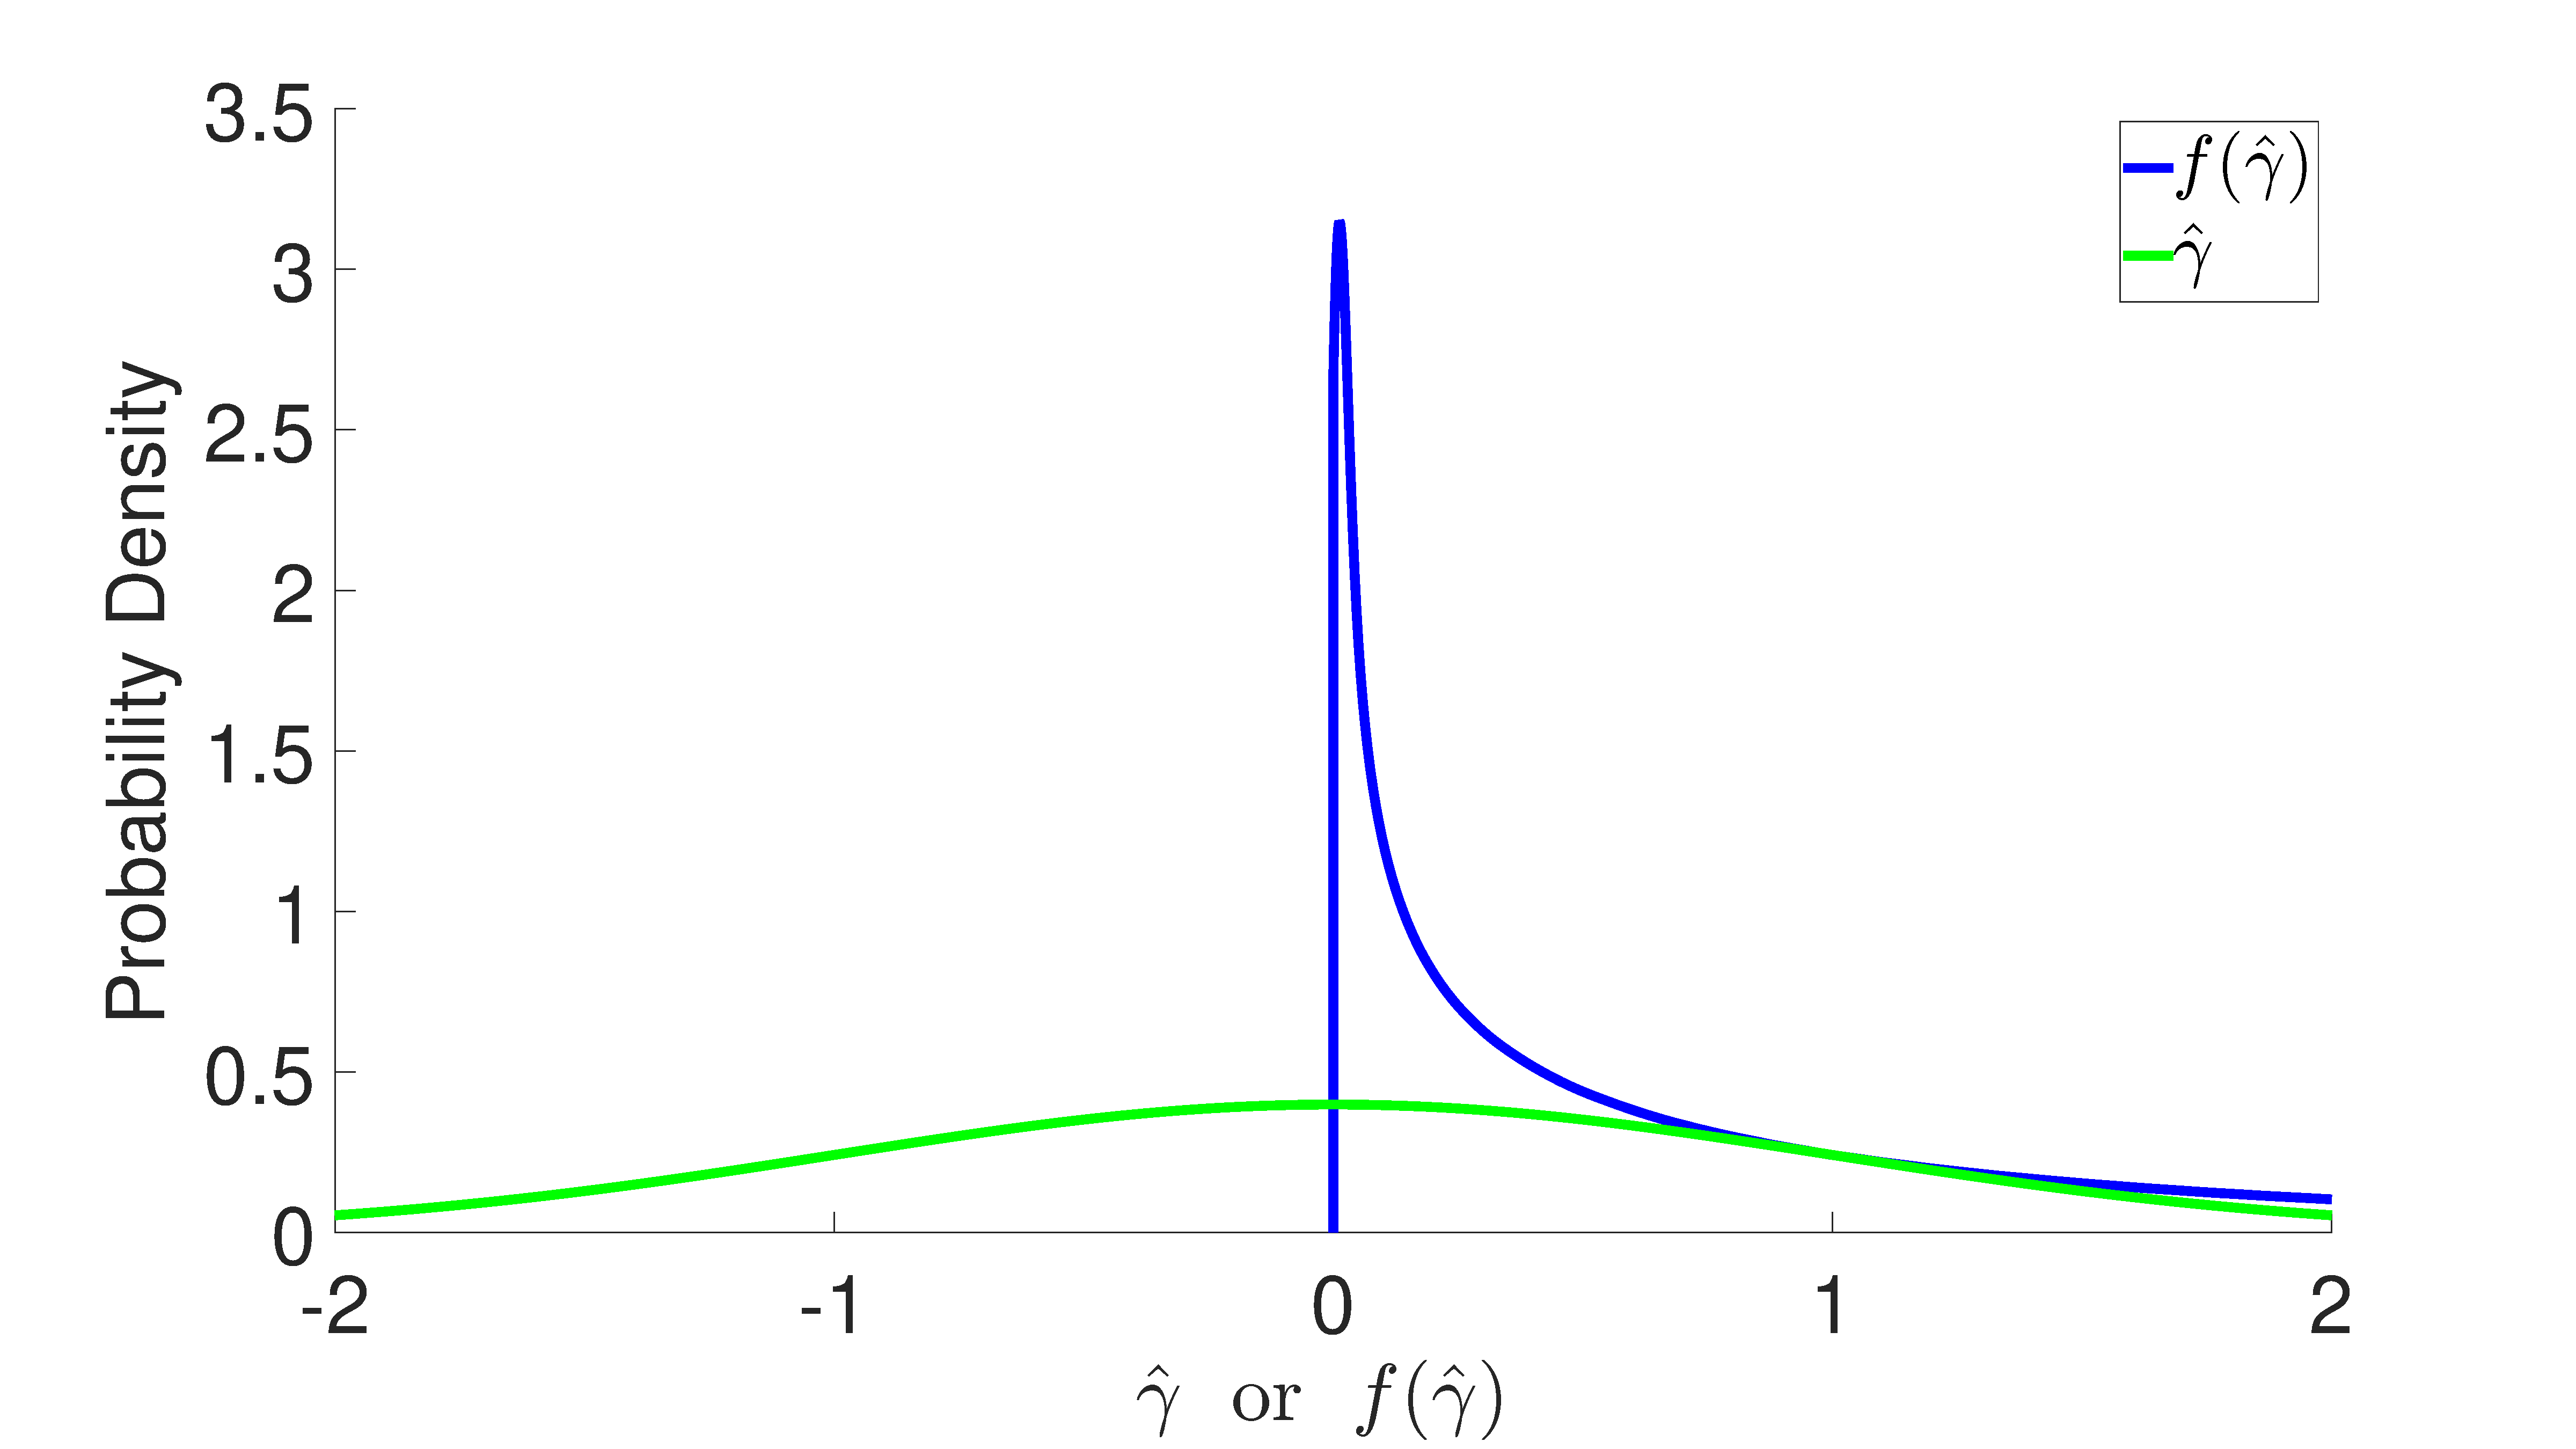
\includegraphics[width=0.5\textwidth]{bias_plot2}
%	\caption{Demonstration of inherent bias.  The true value of $\gamma(y)$ is taken as $0$ for all values of $y$.  Realisations for $\hg$, shown in green, are unbiased and distributed according to a unit Gaussian.  Shown in blue is the distribution of realisation of $f(\hg) = \hg^2$. All instances of $f(\hg)$ are positive and so $\E[f(\hg)]= 1 > 0 = f(\E[\hg])$.  Note also that the function $f'(\hg) = -\hg^2$ would have the opposite bias and so a simple bias correction is not possible.\label{fig:bias-plot}}
%\end{figure}
We now show that 
\emph{any}
strictly convex or concave $f$ entails a biased estimator 
when $\hat{\zeta}_n$ is unbiased but has non-zero variance
given $y_n$. This covers the
case where $\hat{\zeta}_n$ is a MC estimate.
\begin{theorem}
  \label{the:bias-conv}	
  Suppose that $y_n \sim p(y)$ and that each $\hat{\zeta}_n$ satisfies $\E \left[\hat{\zeta}_n \middle| y_n\right] = \gamma(y_n)$.
  Define $\mathcal{A} \subseteq \mathcal{Y}$ as
  $\mathcal{A} = \left\{y \in \mathcal{Y} \;\middle|\; \mathrm{Var}\left(\hat{\zeta}_n \middle| y_n=y \right)>0\right\}$
  and assume that ~$\mathbb{P}(y_n \in \mathcal{A}) > 0$.
  Then for any $f$ that is strictly convex in its second argument,
	\[ 
	\E\left[\frac{1}{N} \sum_{n=1}^N f(y_n, \hat{\zeta}_n)\right] > I(f).
	\]
  Similarly for any $f$ that is strictly concave in its second argument, 
	\[
		\E\left[\frac{1}{N} \sum_{n=1}^N f(y_n, \hat{\zeta}_n)\right] < I(f).
	\]
\end{theorem}
\begin{proof}
	We prove our claim for the case that $f$ is strictly convex; our proof for the other concave case  
	is symmetrical. We have
	\begin{align*}
	\E\left[\frac{1}{N} \sum_{n=1}^N f(y_n, \hat{\zeta}_n)\right] = \E\left[f(y_1, \hat{\zeta}_1)\right] 
	= \E\left[\E\left[f(y_1, \hat{\zeta}_1) \middle| y_1\right]\right] 
	\ge \E\left[f\left(y_1, \E\left[\hat{\zeta}_1 \middle| y_1\right]\right)\right] = I(f)
	%        \E&\left[\frac{1}{N} \sum_{n=1}^N f(y_n, \hat{\zeta}_n)\right] = \E\left[f(y_1, \hat{\zeta}_1)\right] \\
	%        & \quad \quad \quad \quad = \E\left[\E\left[f(y_1, \hat{\zeta}_1)|y_1\right]\right] \\
	%        & \quad \quad \quad \quad = \E\left[\mathbb{I}(y_1 \in \mathcal{A}) \E\left[f(y_1, \hat{\zeta}_1)|y_1\right]\right] \\
	%        & \quad \quad \quad \quad \quad + \E\left[\mathbb{I}(y_1 \notin \mathcal{A}) \E\left[f(y_1, \hat{\zeta}_1)|y_1\right]\right] \\
	%        & \quad \quad \quad \quad \ge \E\left[\mathbb{I}(y_1 \in \mathcal{A}) f\left(y_1, \E\left[\hat{\zeta}_1 \middle| y_1\right]\right)\right] \\
	%        & \quad \quad \quad \quad \quad + \E\left[\mathbb{I}(y_1 \notin \mathcal{A}) \E\left[f(y_1, \hat{\zeta}_1)|y_1\right]\right] \\    
	%        & \quad \quad \quad \quad = \E\left[\E\left[f(y_1, \hat{\zeta}_1)|y_1\right]\right] = I(f)
	\end{align*}
	where the $\ge$ is a result of Jensen's inequality on the inner expectation.  
	Since $f$ is strictly convex and therefore nonlinear, equality holds if and only if
	$\hat{\zeta}_1$ is almost surely constant given $y_1$. 
	This is violated whenever $y_1 \in \mathcal{A}$, which by assumption
	has a non-zero probability of occurring.  Consequently,
	the inequality must be strict, giving the desired result.
\end{proof}
For certain nonlinear $f$, it may still be possible to develop unbiased estimation
schemes using Russian roulette sampling~\citep{lyne2015russian} or other debiasing techniques.  
However, this induces its own complications: for some problems the resultant estimates
have infinite variance \citep{lyne2015russian} and as shown by \cite{jacob2015nonnegative}, there are 
no general purpose ``$f$-factories'' that produce both non-negative and
unbiased estimates for non-constant, positive output functions $f : \real \rightarrow \real^+$,
given unbiased estimates for the inputs.

%This result suggests that general purpose, unbiased inference is impossible for nested
%probabilistic program queries which cannot be mathematically expressed as single inference
%of the form~\eqref{eq:MC}.  Such rearrangement is not possible when the outer query
%depends nonlinearly on a \emph{marginal} of the inner query.  Consequently, query nesting
%using existing systems\footnote{We note that for certain nonlinear $f$, it may still be
%possible to develop an unbiased inference scheme using a combination of a convergent
%Maclaurin expansion and Russian Roulette sampling \cite{lyne2015russian}.} cannot provide
%unbiased estimation of problems that cannot be expressed as a single query.  However, the
%additional models that it does allow expression for, such as the experimental design
%example, might still be estimable in consistent fashion as shown in the previous section.

% !TEX root =  main.tex

\section{Empirical Verification}
\label{sec:empirical}

The convergence rates proven in Section~\ref{sec:convergence} are only
\emph{upper bounds} on the worst-case performance we can expect. We will now
examine whether these convergence rates are tight in practice, investigate what happens
when our guidelines are not followed, and examine the effect of different strategies for
choosing $N_k$ under a sample budget.  We note that one of the main applications of
our results is provided later in Chapter~\ref{chp:design}, while an additional real-world
example is given in~\citep{rainforth2017pitfalls}.


\subsection{Simple Analytic Model}
\label{sec:simple}

We start with the following simple analytically calculable problem
\begin{equation}
\begin{aligned}
\label{eq:model}
& y \sim \mathrm{Uniform}(-1,1), &&
z \sim \mathcal{N}(0,1), \\
& \phi(y,z) = \sqrt{2/\pi}\exp\left(-2(y-z)^2\right), &&
f(y,\gamma(y)) = \log (\gamma (y)) = \log(\E_z[\phi(y,z)]).
\end{aligned}
\end{equation}
for which $I = \mathbb{E}_{p(y)}\left[f\left(y,\mathbb{E}_{p(z|y)}
\left[\phi(y,z)\right]\right)\right]=\frac{1}{2}\left(\log(2)-\log(5)-\log(\pi)\right)-\frac{2}{15}$.
Figure~\ref{fig:emprical-conv} shows the corresponding empirical convergence obtained by
applying~\eqref{eq:nested-mc} to~\eqref{eq:model} directly. It shows that for this
problem the theoretical convergence rates from Theorem~\ref{the:Repeat} are indeed
realized.\footnote{Note the continuous differentiability assumption is satisfied as $\gamma(y)\neq0$
or $\infty$ for any $y\in[-1,1]$.}
The figure also demonstrates the danger of not increasing
$M$ with $N$, showing that the NMC estimator converges to an incorrect solution when $M$
is held constant.  Figure~\ref{fig:tau_sweep} shows the effect of varying $N$ and $M$ for various
fixed sample budgets $T$ and demonstrates that the asymptotically optimal strategy can be suboptimal
for finite budgets.

\begin{figure}[t]
	\centering
	\begin{subfigure}[b]{0.49\textwidth}
		\centering
	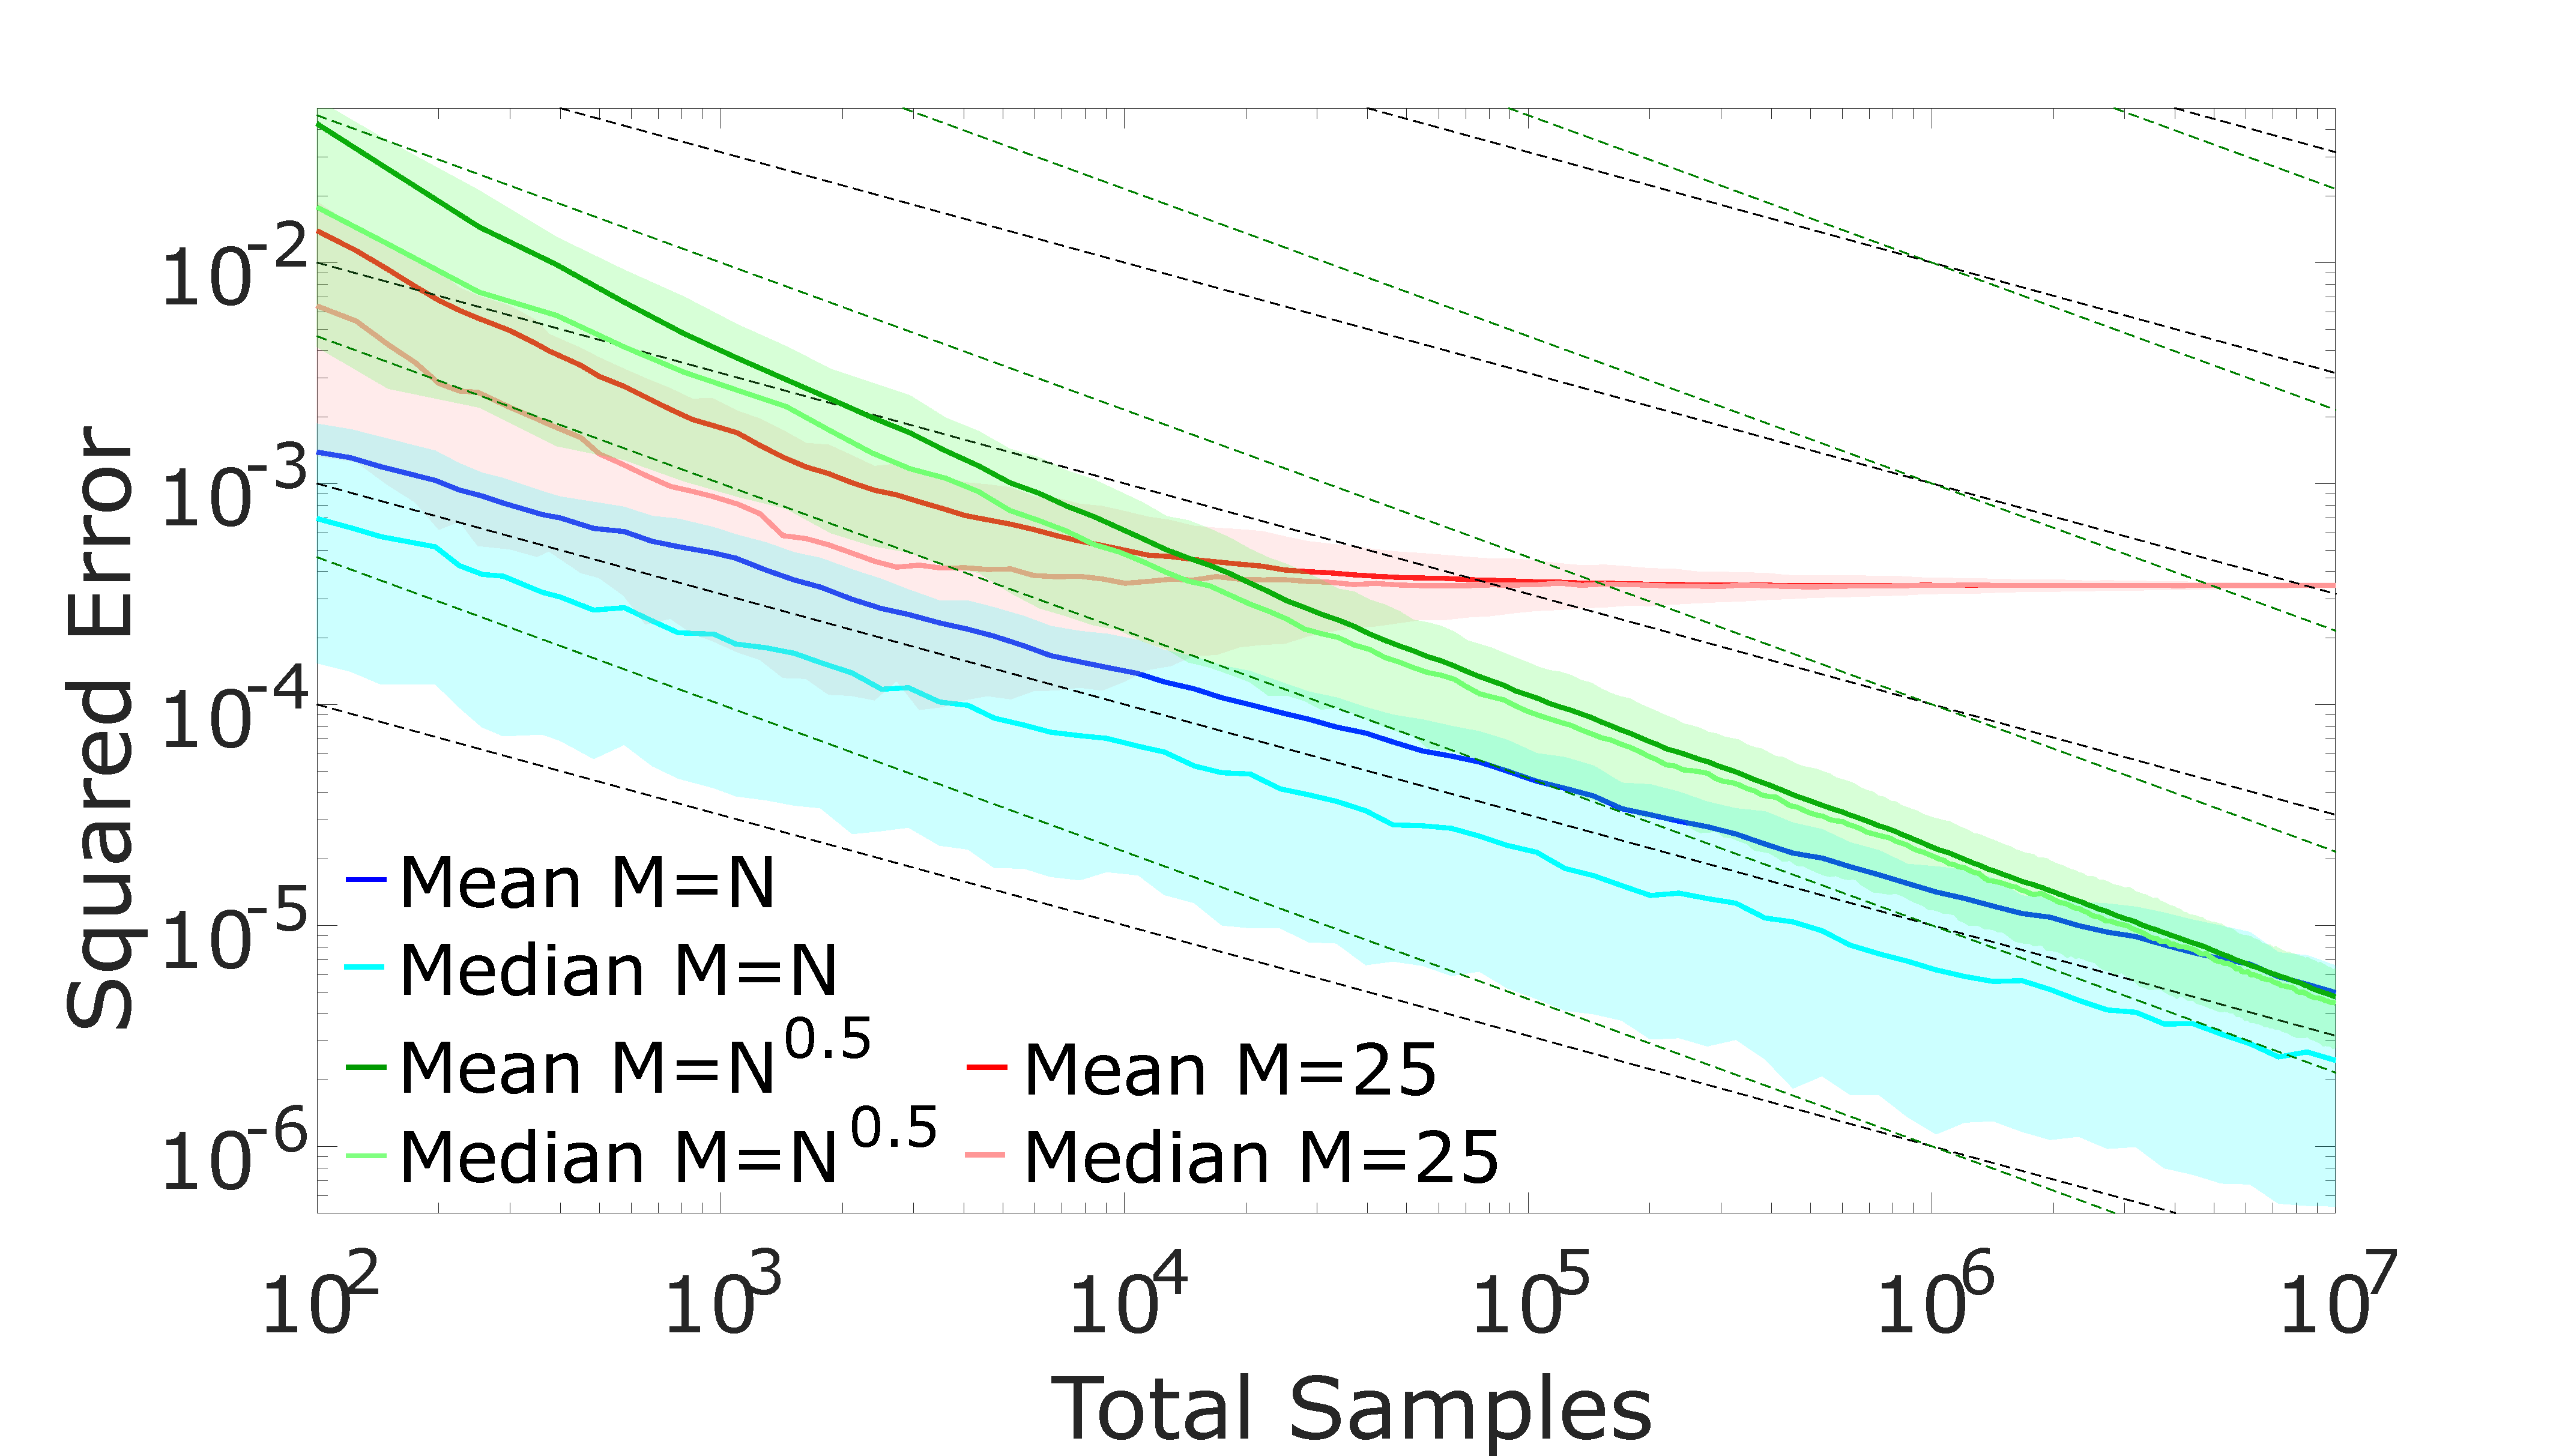
\includegraphics[width=0.99\textwidth,trim={1.5cm 0 3.5cm 0},clip]{gaussian_conv2}
	\caption{Convergence of NMC for different $\tau$. \label{fig:emprical-conv}}
	\end{subfigure}
	\begin{subfigure}[b]{0.49\textwidth}
		\centering
	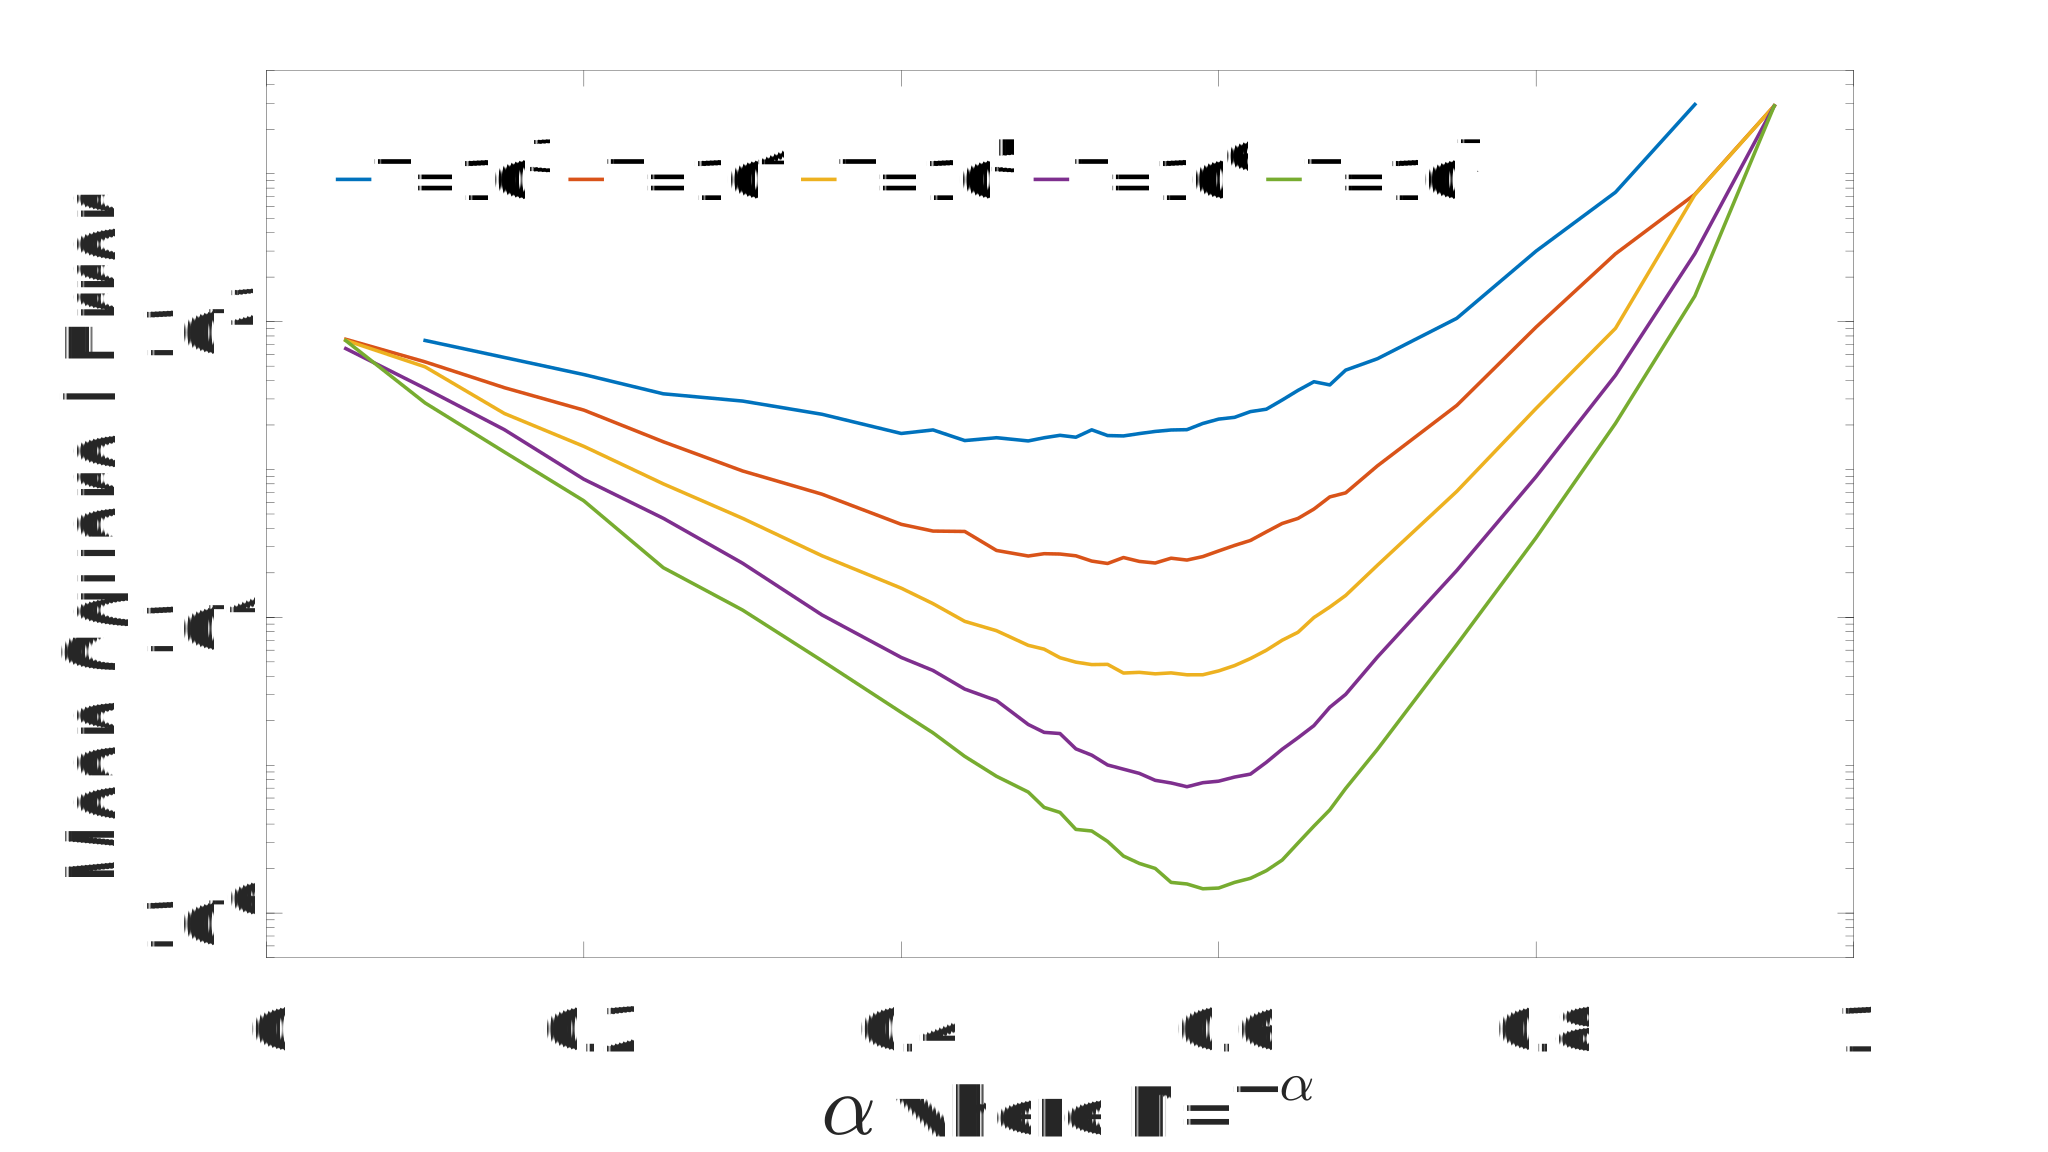
\includegraphics[width=0.99\textwidth,trim={1.5cm 0 3.5cm 0},clip]{tau_sweep}
		\caption{Final error for different $T$ and $N$.\label{fig:tau_sweep}}
	\end{subfigure}
	\vspace{5pt}
	\caption{Empirical convergence of NMC for~\eqref{eq:model}.  Shown left is the
		convergence in total samples for different ways of setting $M$ and $N$.  
		Results are averaged over 1000 independent runs, while shaded regions give the 25\%-75\% quantiles. We
		see that the theoretical convergence rates (as shown by the dash lines) are observed. 
		The fixed $M$ case converges at the \mc error rate, but to a biased solution.
		Shown right is the final error for different total sample budgets
		as a function of $\alpha$ where $N=T^{\alpha}$ and $M=T^{1-\alpha}$ iterations are used for the outer
		and inner estimators respectively.  This shows that even though $\alpha=2/3$ is the
		asymptotically optimal allocation strategy, this is not the optimal solution for
		finite $T$. Nonetheless, as $T$ increases, the optimum value of $\alpha$ increases,
		starting at around $0.5$ for $T=10^3$ and reaching around $0.6$ for $T=10^7$. \vspace{-5pt}}
\end{figure}	

% !TEX root =  main.tex

\subsection{Repeated Nesting}
\label{sec:exp-repeat-app}

We next consider some simple models with multiple levels of nesting, starting with
\begin{subequations}
	\label{eq:repeat-nest}
\begin{align}
y^{(0)} \sim \mathrm{Uniform}(0,1), \quad &
y^{(1)} \sim \mathcal{N}(0,1), \quad
y^{(2)} \sim \mathcal{N}(0,1), \displaybreak[0] \\ 
f_0 \left(y^{(0)}, \gamma_1\left(y^{(0)}\right)\right)&= \log \gamma_1\left(y^{(0)}\right) \displaybreak[0] \\ 
f_1 \left(y^{(0:1)}, \gamma_2\left(y^{(0:1)}\right)\right)&= 
\exp\left(-\frac{1}{2}\left(y^{(0)}-y^{(1)}-\log \gamma_2\left(y^{(0:1)}\right)\right)\right) \displaybreak[0] \\ 
f_2 \left(y^{(0:2)}\right)&=\exp\left(y^{(2)}-\frac{y^{(0)}+y^{(1)}}{2}\right)
\end{align}
\end{subequations}
which has analytic solution $I=\E \left[f_0 \left(y^{(0)},\E \left[f_1 \left(y^{(0:1)},\E \left[f_2\left(y^{(0:2)}\right) \middle| 
y^{(0:1)}\right]\right) \middle| y^{(0)}\right]\right)\right]=-3/32$. 
The converge plot shown in Figure~\ref{fig:multi-nest} shows that the
theoretically expected convergence\footnote{Strictly speaking the assumptions of Theorem~\ref{fig:multi-nest} are
	not actually satisfied for this model and the later modifications
	 because $K_1 = C_1 = \infty$.  However, we see convergence behavior
	as if the assumptions were satisfied.  This highlights the importance of Theorem~\ref{the:Consistent}
	because $f_1$ does satisfy this weaker assumption.}
behaviors are observed for different methods of setting 
$N_0, N_1$, and $N_2$.

\begin{figure}[t]
	\centering
	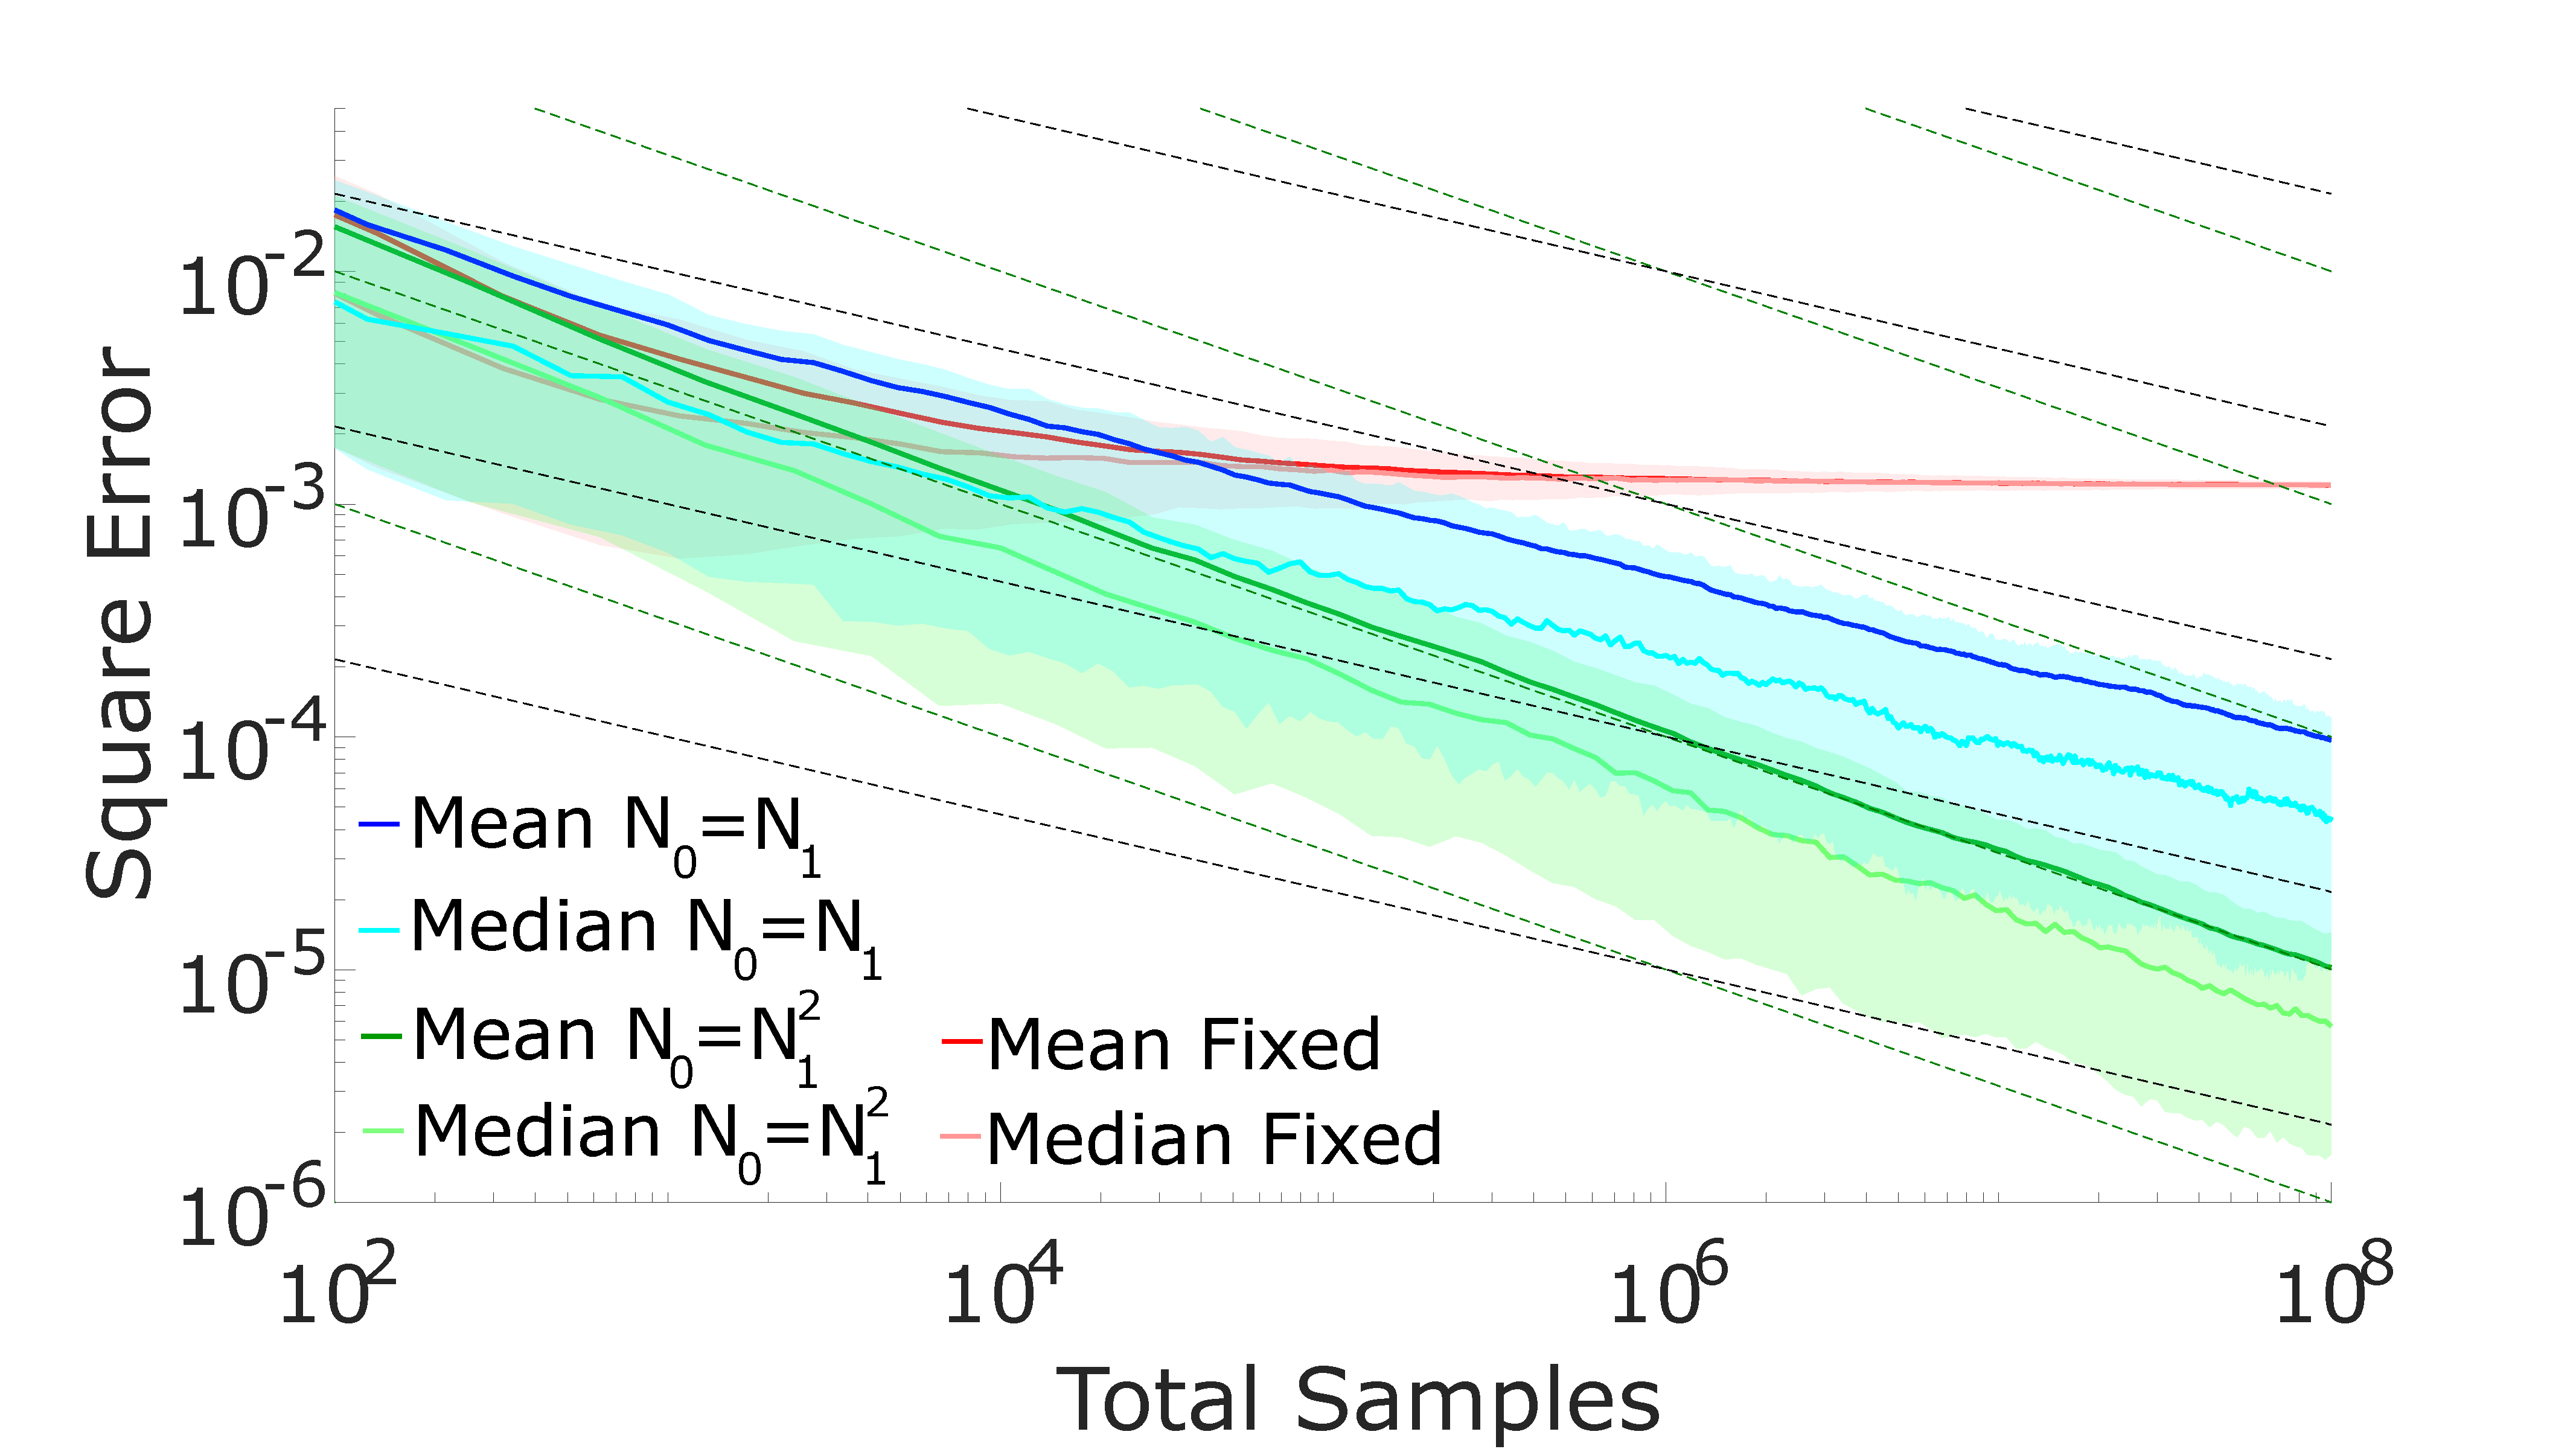
\includegraphics[width=0.5\textwidth,trim={1.5cm 0 3.5cm 0},clip]{repeat_nest_an}
	\caption{Empirical convergence of NMC to~\eqref{eq:repeat-nest} for an increasing total sample budget
		$T=N_0 N_1 N_2$.  Results are averaged over 1000 independent runs, while shaded regions give the 25\%-75\% quantiles.
		Shown in red is the convergence with a fixed $N_2=5$ and $N_1=N_2^2$, for which we see gives convergence
		to a biased solution, such that the error remains bounded as $T$ increases.  Shown in blue is the convergence
		when setting $N_0=N_1=N_2$, which we see converges at the expected $O(T^{-1/3})$ rate.  The black dashed lines
		provide a reference for this expected convergence of this estimator.  Shown in green is the convergence when
		setting $N_0=N_1^2=N_2^2$ which we seen again gives the theoretical convergence rate, this time $O(T^{-1/2})$
		with the dashed green lines providing reference.\label{fig:multi-nest}}
\end{figure}	

We next consider the empirical performance of different strategies for choosing $N_0, N_1$, $N_2$ under a 
finite fixed budget $T=N_0N_1N_2$.
To do this, we define $\alpha_1$ and $\alpha_2$ such that $N_0 = T^{\alpha_1}$, 
$N_1 = T^{\alpha_2(1-\alpha_1)}$, and $N_2 = T^{(1-\alpha_1)(1-\alpha_2)}$ and then consider the variation in the
mean squared error with $(\alpha_1,\alpha_2)$.  In particular, we look to establish the optimal empirical
setting under the fixed budget $T=10^6$.  To investigate how sensitive the empirically optimal 
allocation is to the problem at hand, we consider both the model described in~\eqref{eq:repeat-nest} and 
also two slight variations.  The first keeps everything the same as~\eqref{eq:repeat-nest} except the following replacements
\begin{subequations}
	\label{eq:repeat-nest2}
	\begin{align}
		y^{(0)} &\sim \mathrm{Uniform}(-1,1), \\
		f_2 \left(y^{(0:2)}\right)&=\exp\left(\frac{y^{(1)}+y^{(2)}-y^{(0)}}{2}\right)
	\end{align}
\end{subequations}
while the second instead replaces $y^{(0)}$ with $y^{(0)}/10$ in the definitions of $f_1$ and $f_2$.  The two
respectively have analytic solutions of $I=11/32$ and $I=39/160$.

To 
try and find the optimal $(\alpha_1,\alpha_2)$ and establish the variation of the MSE more generally,
we ran a Bayesian optimization
algorithm (specifically the ``Black-box Bayesian optimization'' algorithm of~\cite{rainforth2015workshopbopp}) to
optimize the mean squared error, estimated by averaging $1000$ trials at each iteration, with respect to 
$(\alpha_1,\alpha_2)$.  This produced the performance characterizations shown in
Figure~\ref{fig:multi-tau}, corresponding to contour plots of $\log_{10} \left(\E \left[(I_0-\gamma_0)^2\right]\right)$ as
estimated by the surrogate function generated after $200$ Bayesian optimization iterations.
It further found respective optimal values for $(\alpha_1,\alpha_2)$ of  $(0.53,0.36)$, $(0.55,0.69)$, and $(0.38,0.45)$,
giving corresponding values for $(N_0,N_1,N_2)$
of $(1563,10,64)$, $(1957,73,7)$, and $(192,47,111)$.\footnote{Note that there is inevitably a small bias introduced
	by the fact that each $N_k$ has to be a whole number.  The true values of $T$ used for these solutions
	were $1000320,\; 1000027,$ and $1001664$ respectively.}  By comparison, the asymptotically optimal
setup suggested by our theoretical results is $\alpha_1=\alpha_2=0.5$ giving $N_0=977$, $N_1=32$, and 
$N_2=32$.
This demonstrates that even for relatively large values of $T$, the finite budget optimal allocation can vary significantly
from the asymptotically optimal solution.  We also see that the relative optimally can change quite significantly with
changes to the target problem.  For example, the second modification meant it was more preferable to run less iterations of
the outer estimator, perhaps because it reduced the relative importance of $y^{(0)}$ compared to the other variables
in $f_1$ and $f_2$.  However, further work is required to
establish concrete empirical guidelines and investigate whether methods that adaptively allocate the number of
samples might be feasible.  In the meantime, the asymptotically optimal choice (presuming continuous differentiability) 
of $N_0 \propto N_1^2 \propto \dots \propto N_D^2$ seems to a reasonable practical choice on average.

\begin{figure}[t]
	\centering
	\begin{subfigure}[b]{0.32\textwidth}
		\centering
		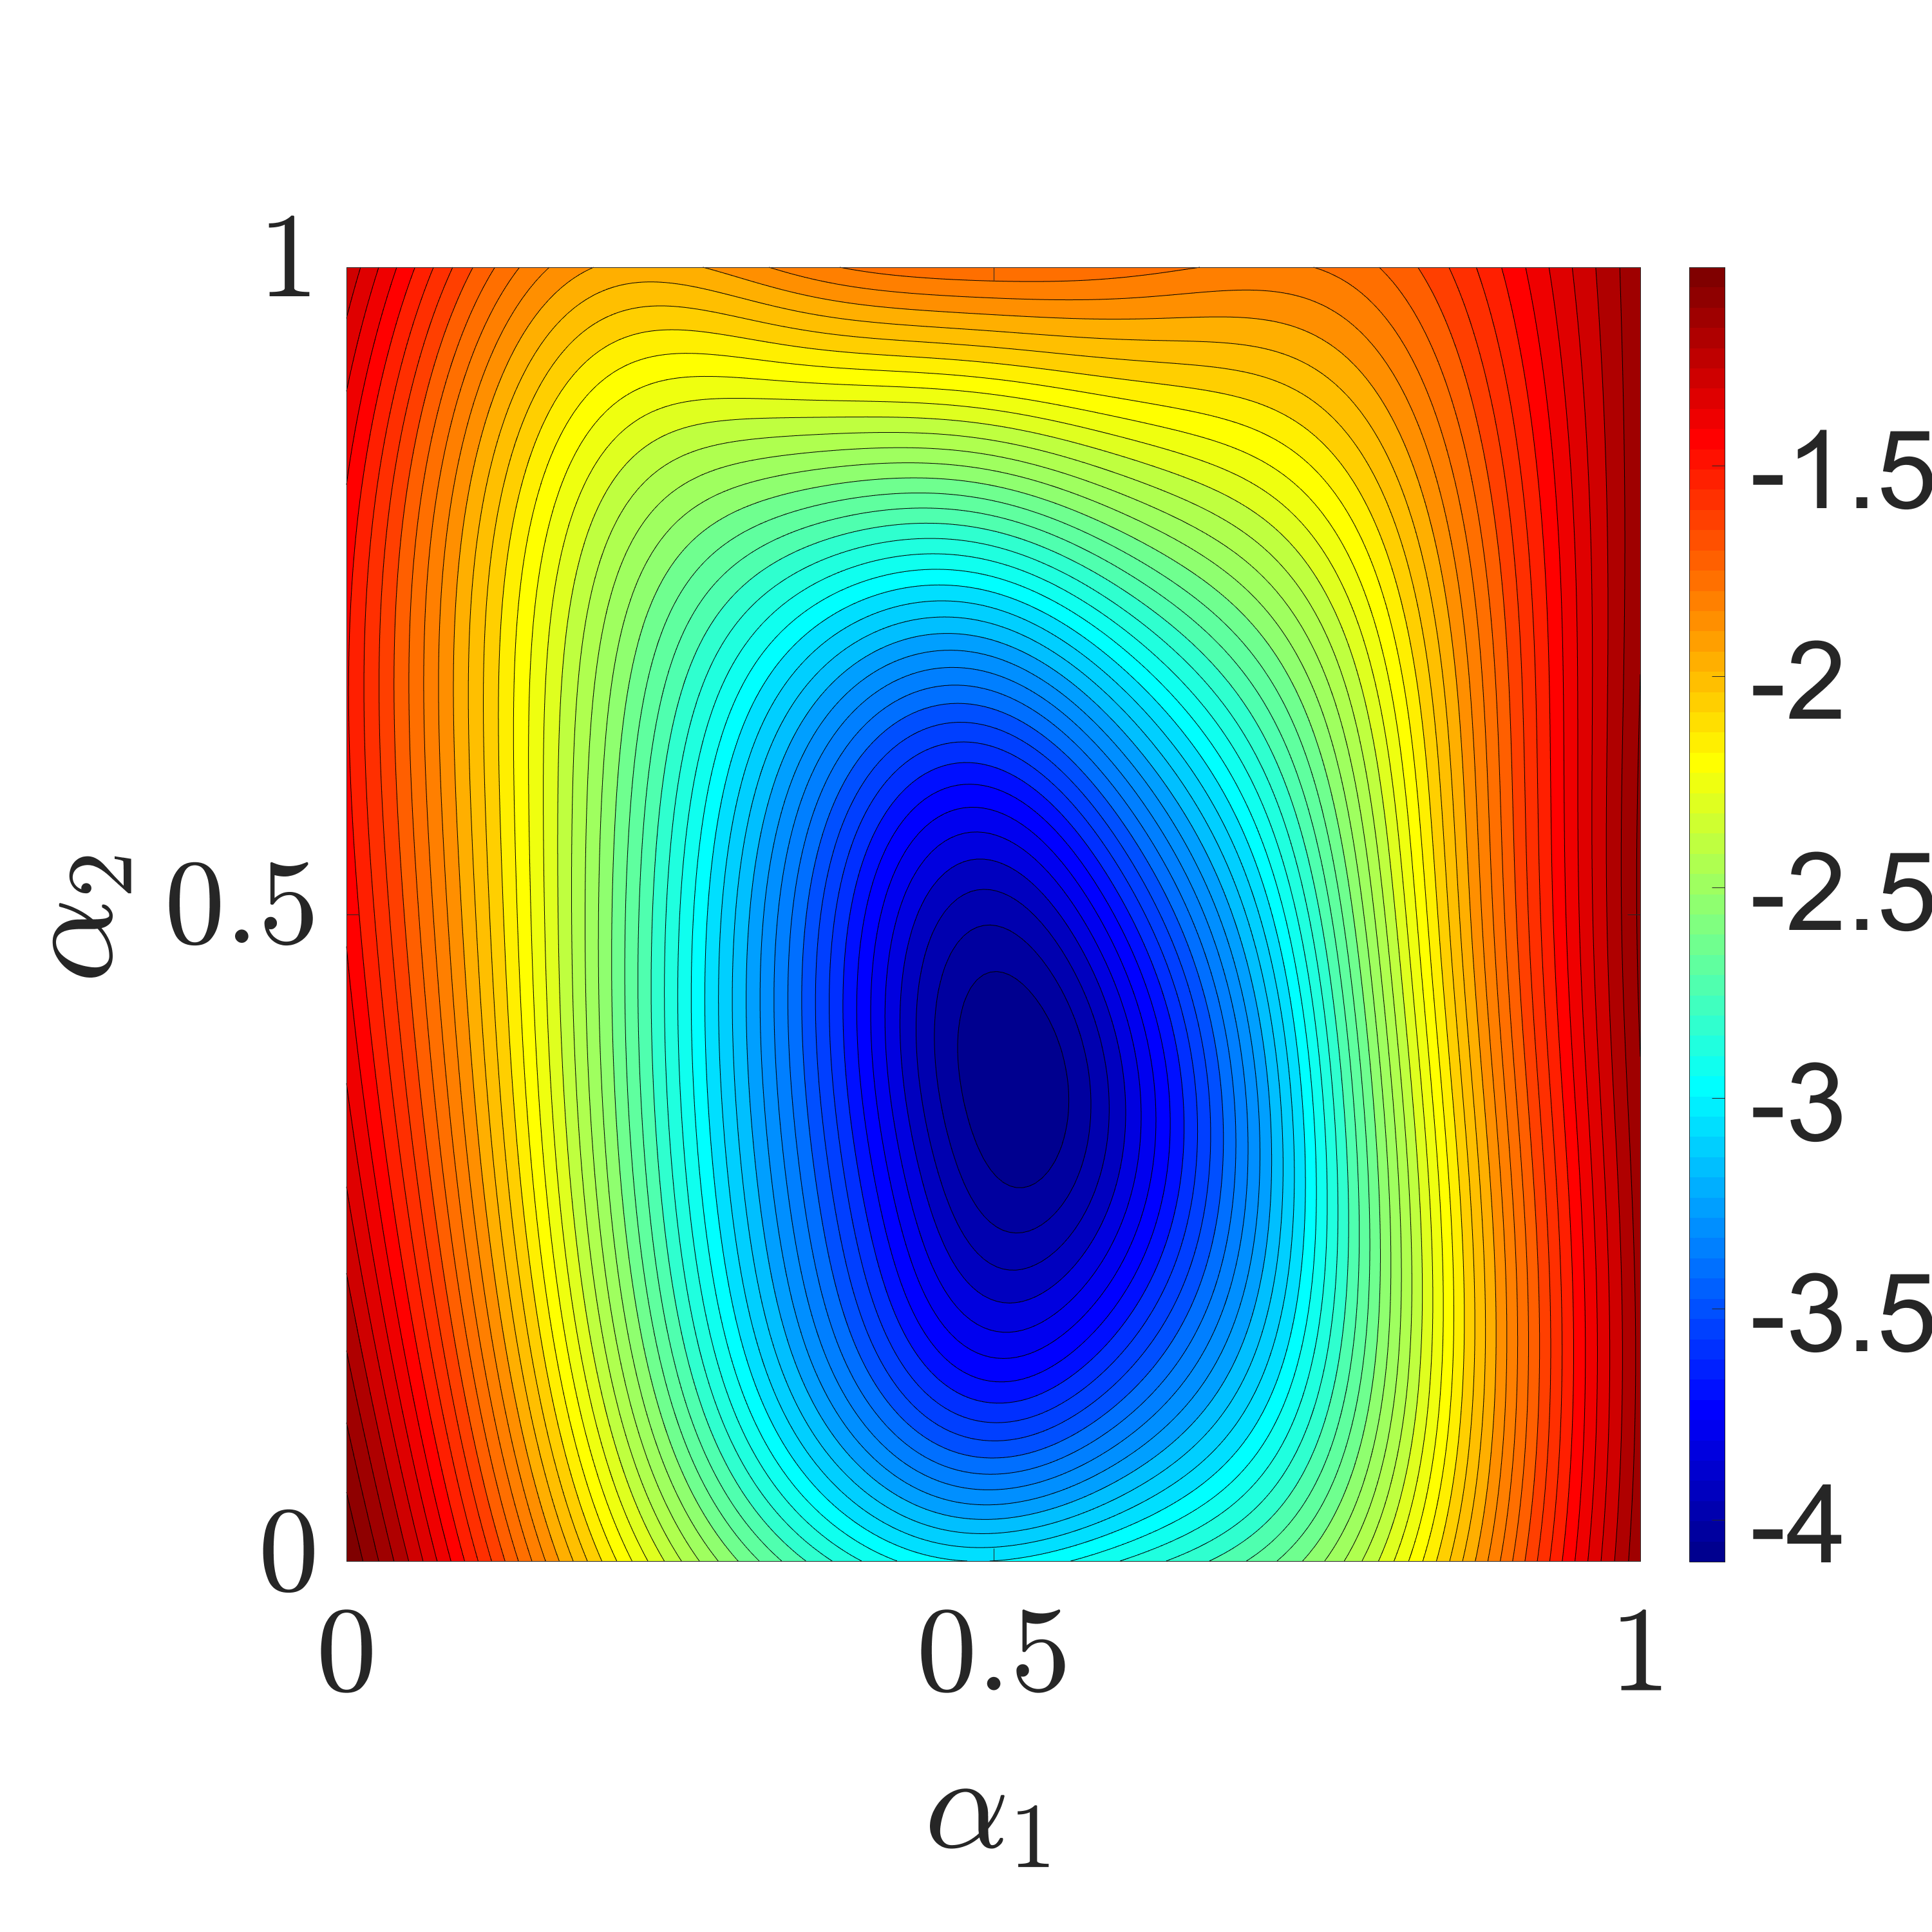
\includegraphics[height=0.88\textwidth]{tmax_1e6_model_3_contour_plot.pdf}
		\caption{Original}
	\end{subfigure}
	~\hspace{4pt}
	\begin{subfigure}[b]{0.32\textwidth}
		\centering
		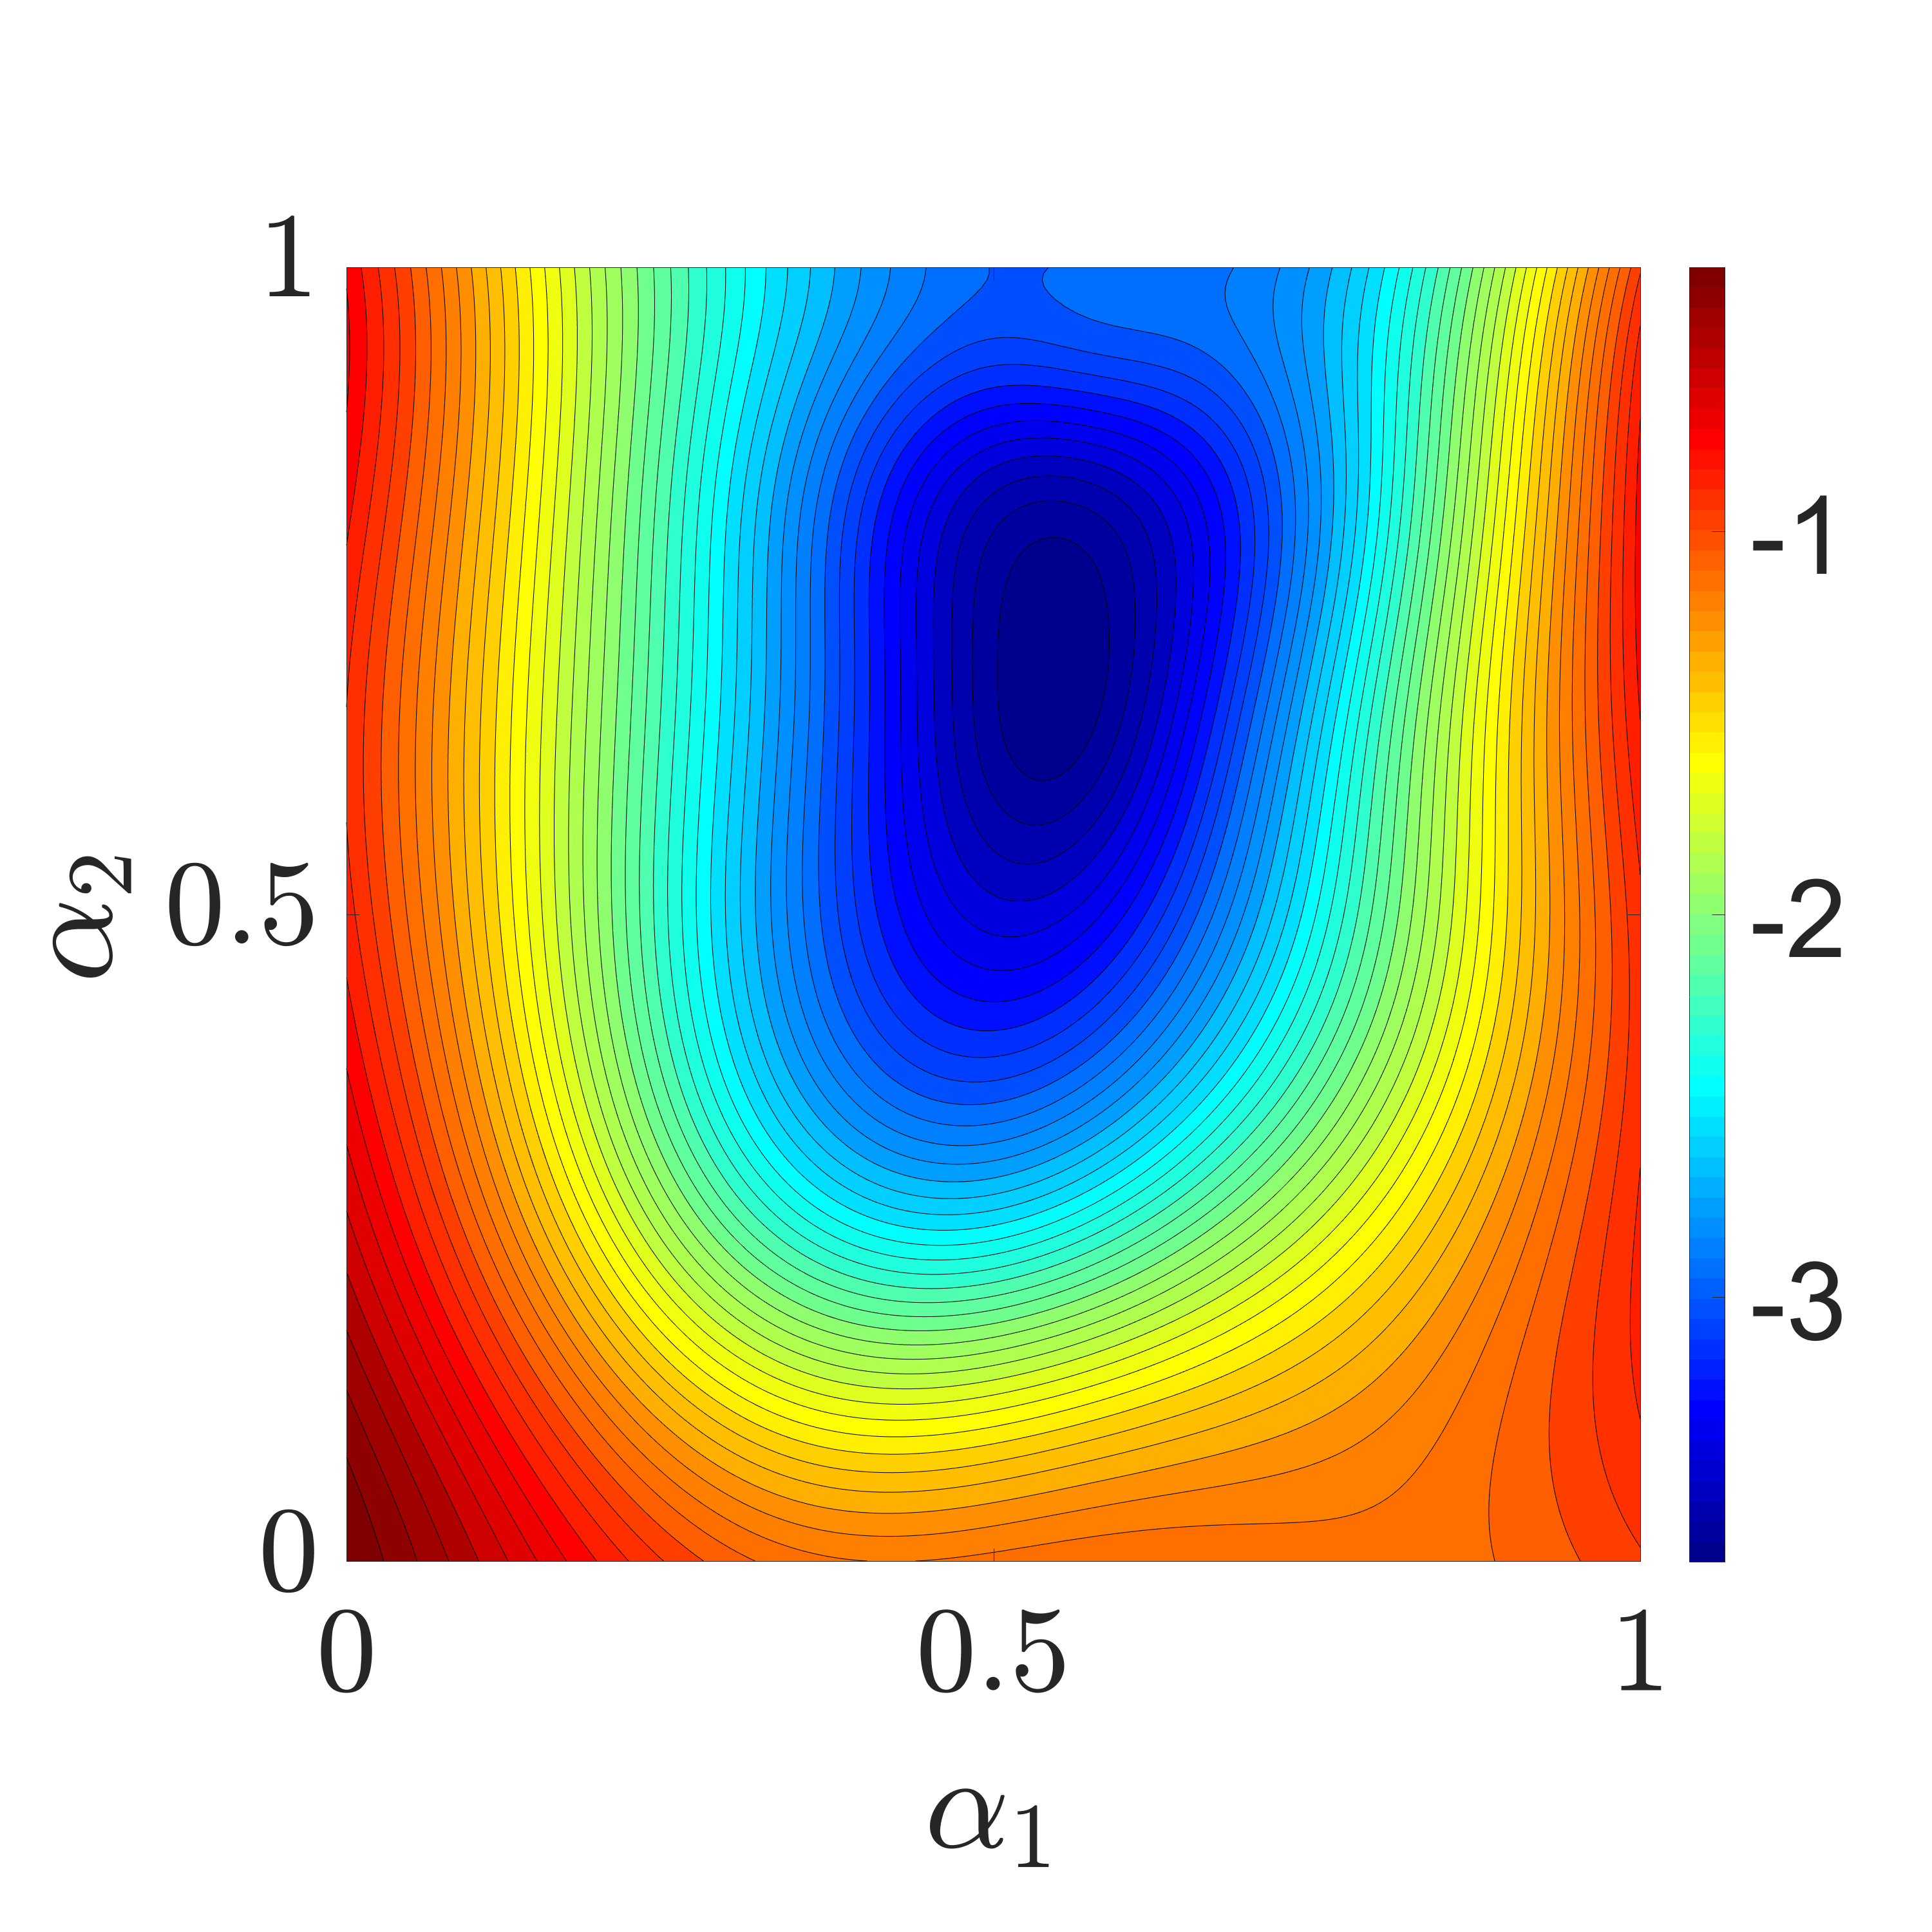
\includegraphics[height=0.88\textwidth]{tmax_1e6_model_2_contour_plot.pdf}
		\caption{First modification}
	\end{subfigure}
	~\hspace{-3pt}
	\begin{subfigure}[b]{0.32\textwidth}
		\centering
		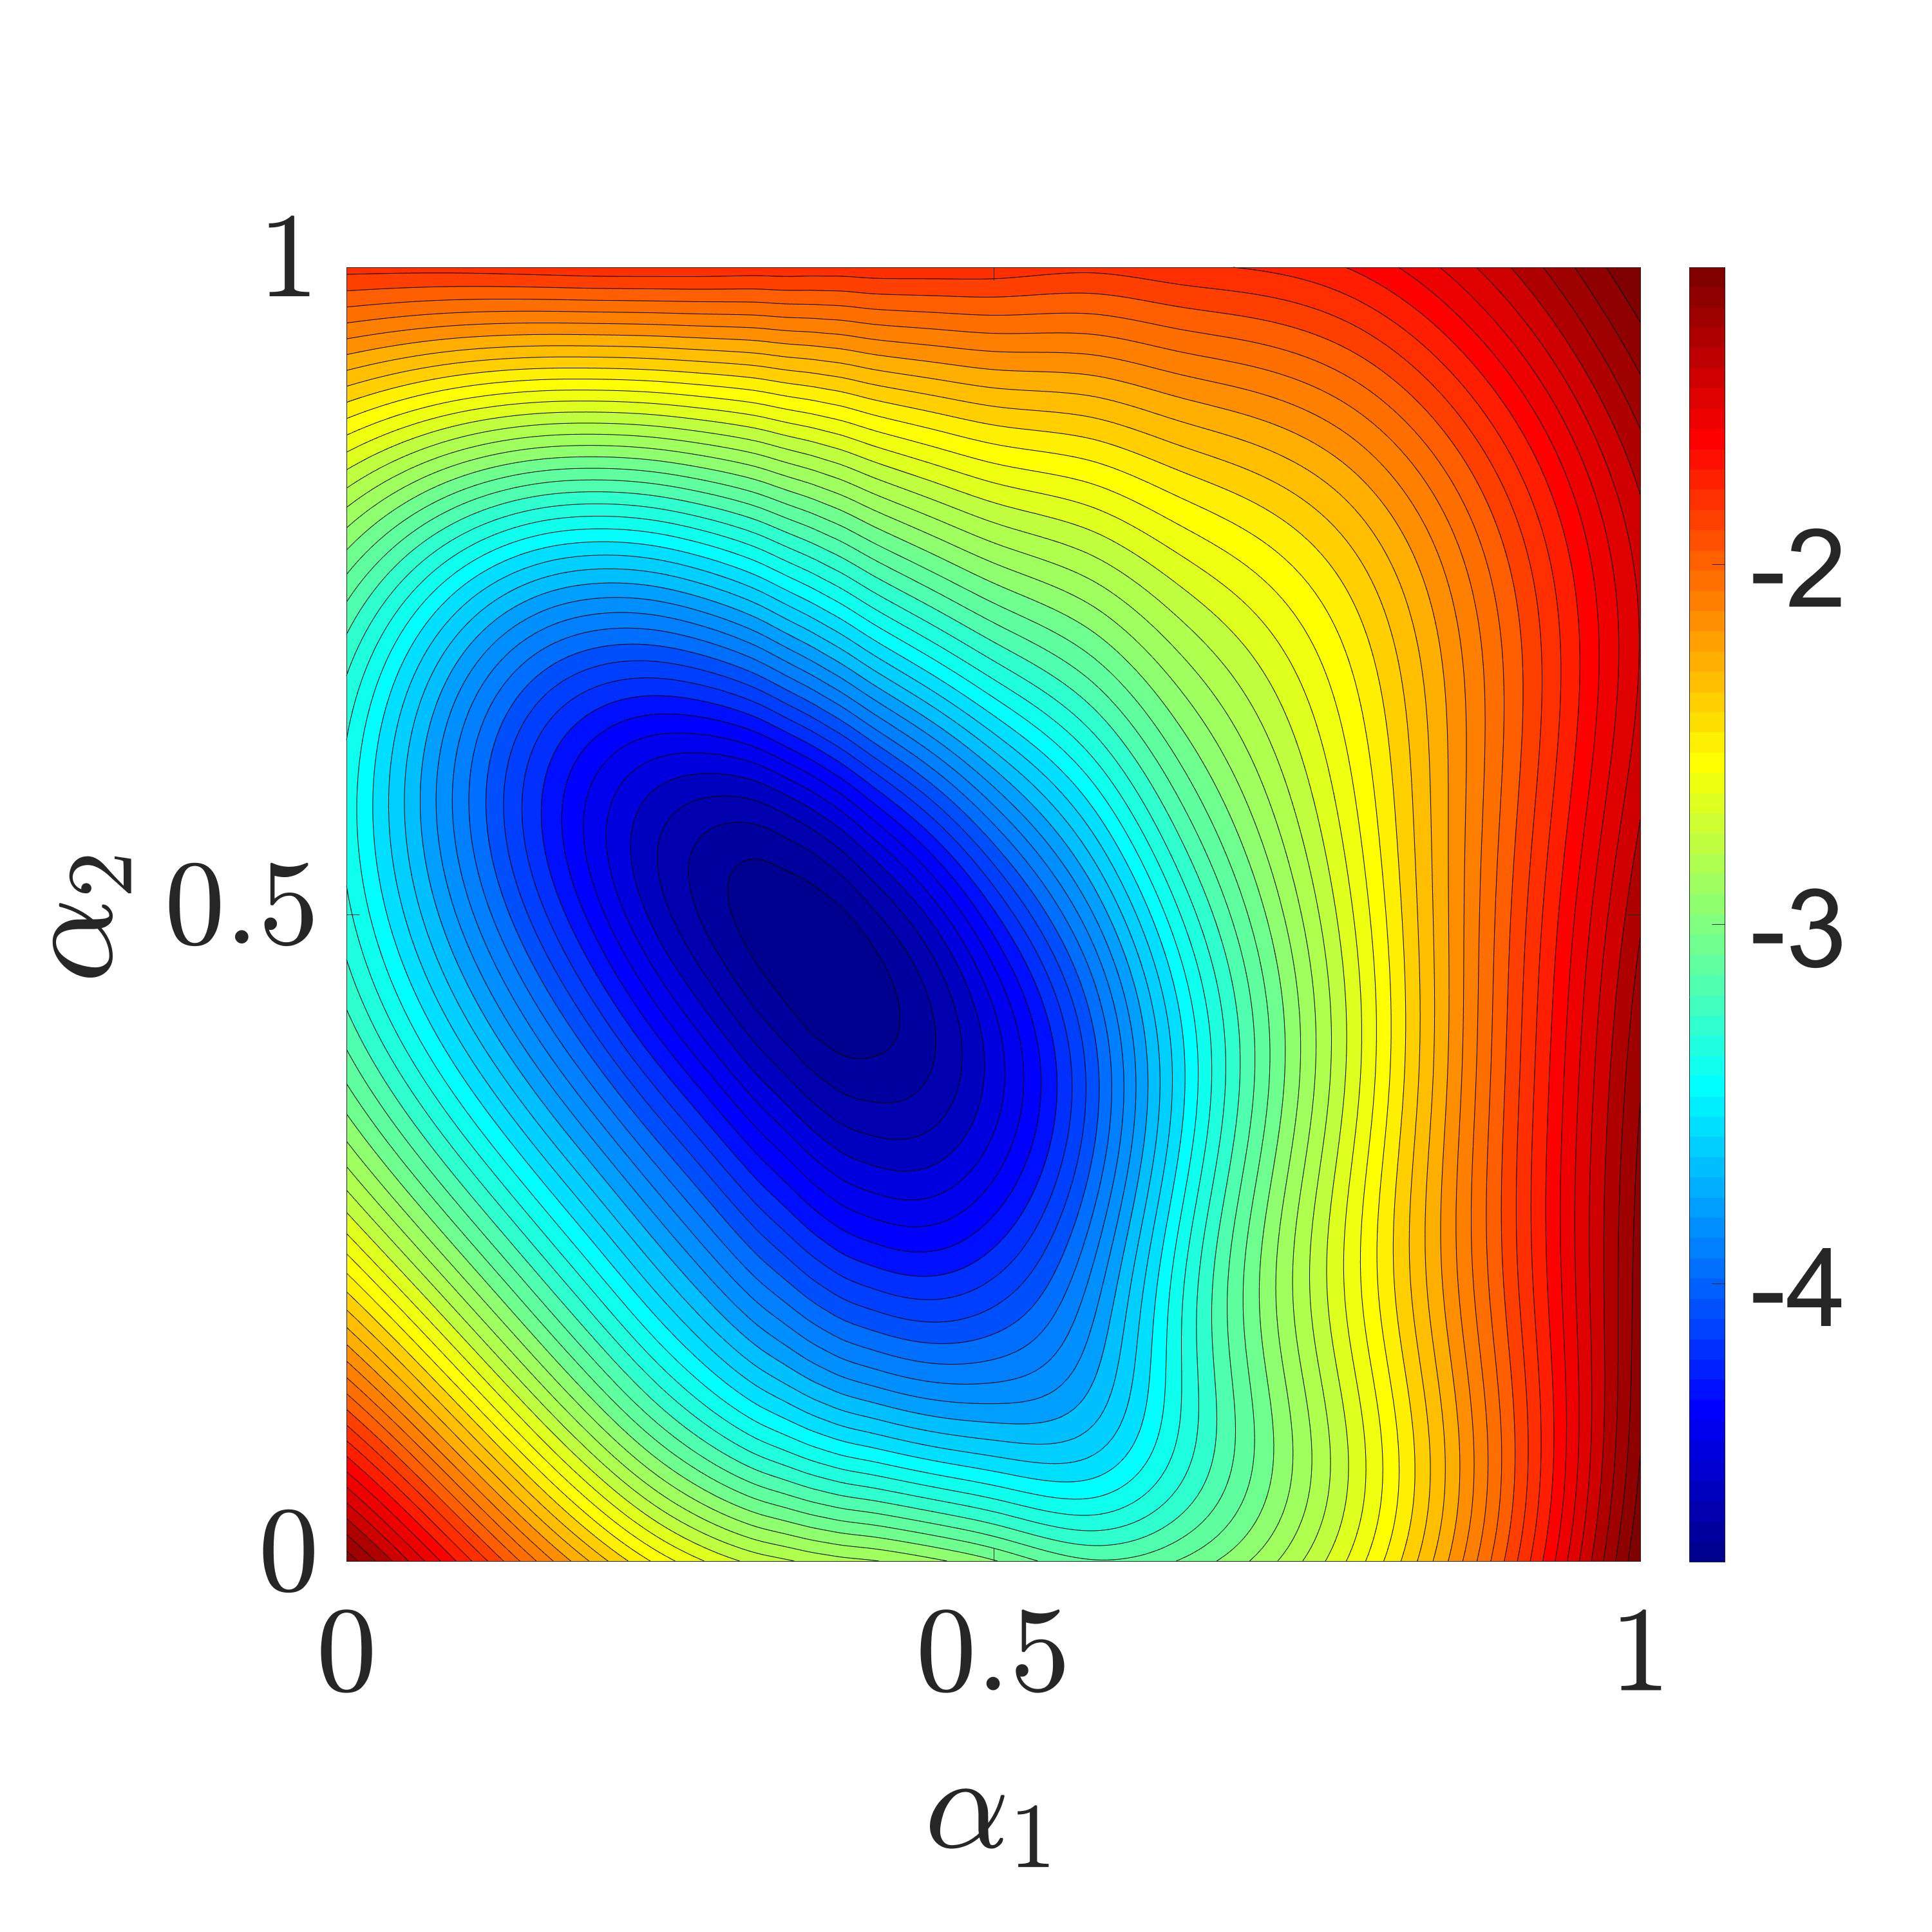
\includegraphics[height=0.88\textwidth]{tmax_1e6_model_4_contour_plot.pdf}
		\caption{Second modification}
	\end{subfigure}
	\caption{Contour plots of $\log_{10} \left(\E \left[(I_0-\gamma_0)^2\right]\right)$ (i.e. $\log_{10}$ MSE, estimated
		by averaging over $1000$ individual estimations)
		for different allocations of the sample budget $T=10^6$ between $N_0$, $N_1$,
		and $N_2$ for problem shown in~\eqref{eq:repeat-nest} and two modifications explained in
		the text.
		\label{fig:multi-tau}}
\end{figure}	
%
%\subsection{Planning Cancer Treatment}
%\label{sec:cancer}
%
%We now introduce a real-world example to show the applicability of NMC in a scenario
%where the solution is not analytically tractable and conventional \mc is insufficient.
%Consider a treatment center assessing a new policy for planning cancer treatments, subject to a budget. 
%Clinicians must decide on a patient-by-patient basis whether to administer chemotherapy in the
%hope that their tumor will reduce in size sufficiently to be able to perform surgery at a later date.
%A treatment is considered to have been successful if the size of the tumor drops below a threshold value in a fixed time window.
%The clinicians have at their disposal a simulator for the evolution of tumors with time,
%parameterized by both observable values, $y$, such as tumor size, and unobservable values, $z$, such as the patient-specific response to treatment.
%Given a set of input parameters, the simulator deterministically returns a binary response $\phi(y,z)\in\left\lbrace 0,1\right\rbrace $, with $\phi(y,z) = 1$ indicating a successful treatment.
%To estimate the probability of a successful treatment for a given patient, the clinician must calculate the expected
%success over these unobserved variables, namely $\E_{p(z|y)} [\phi(y,z)]$ where $p(z|y)$ represents a probabilistic
%model for the unobserved variables, which could, for example, be constructed based on empirical data.
%The clinician then decides whether to go ahead with the treatment for that
%patient based on whether the calculated probability of success exceeds a certain threshold $T_{\mathrm{treat}}$.
%
%\begin{figure}[t]
%	\centering
%		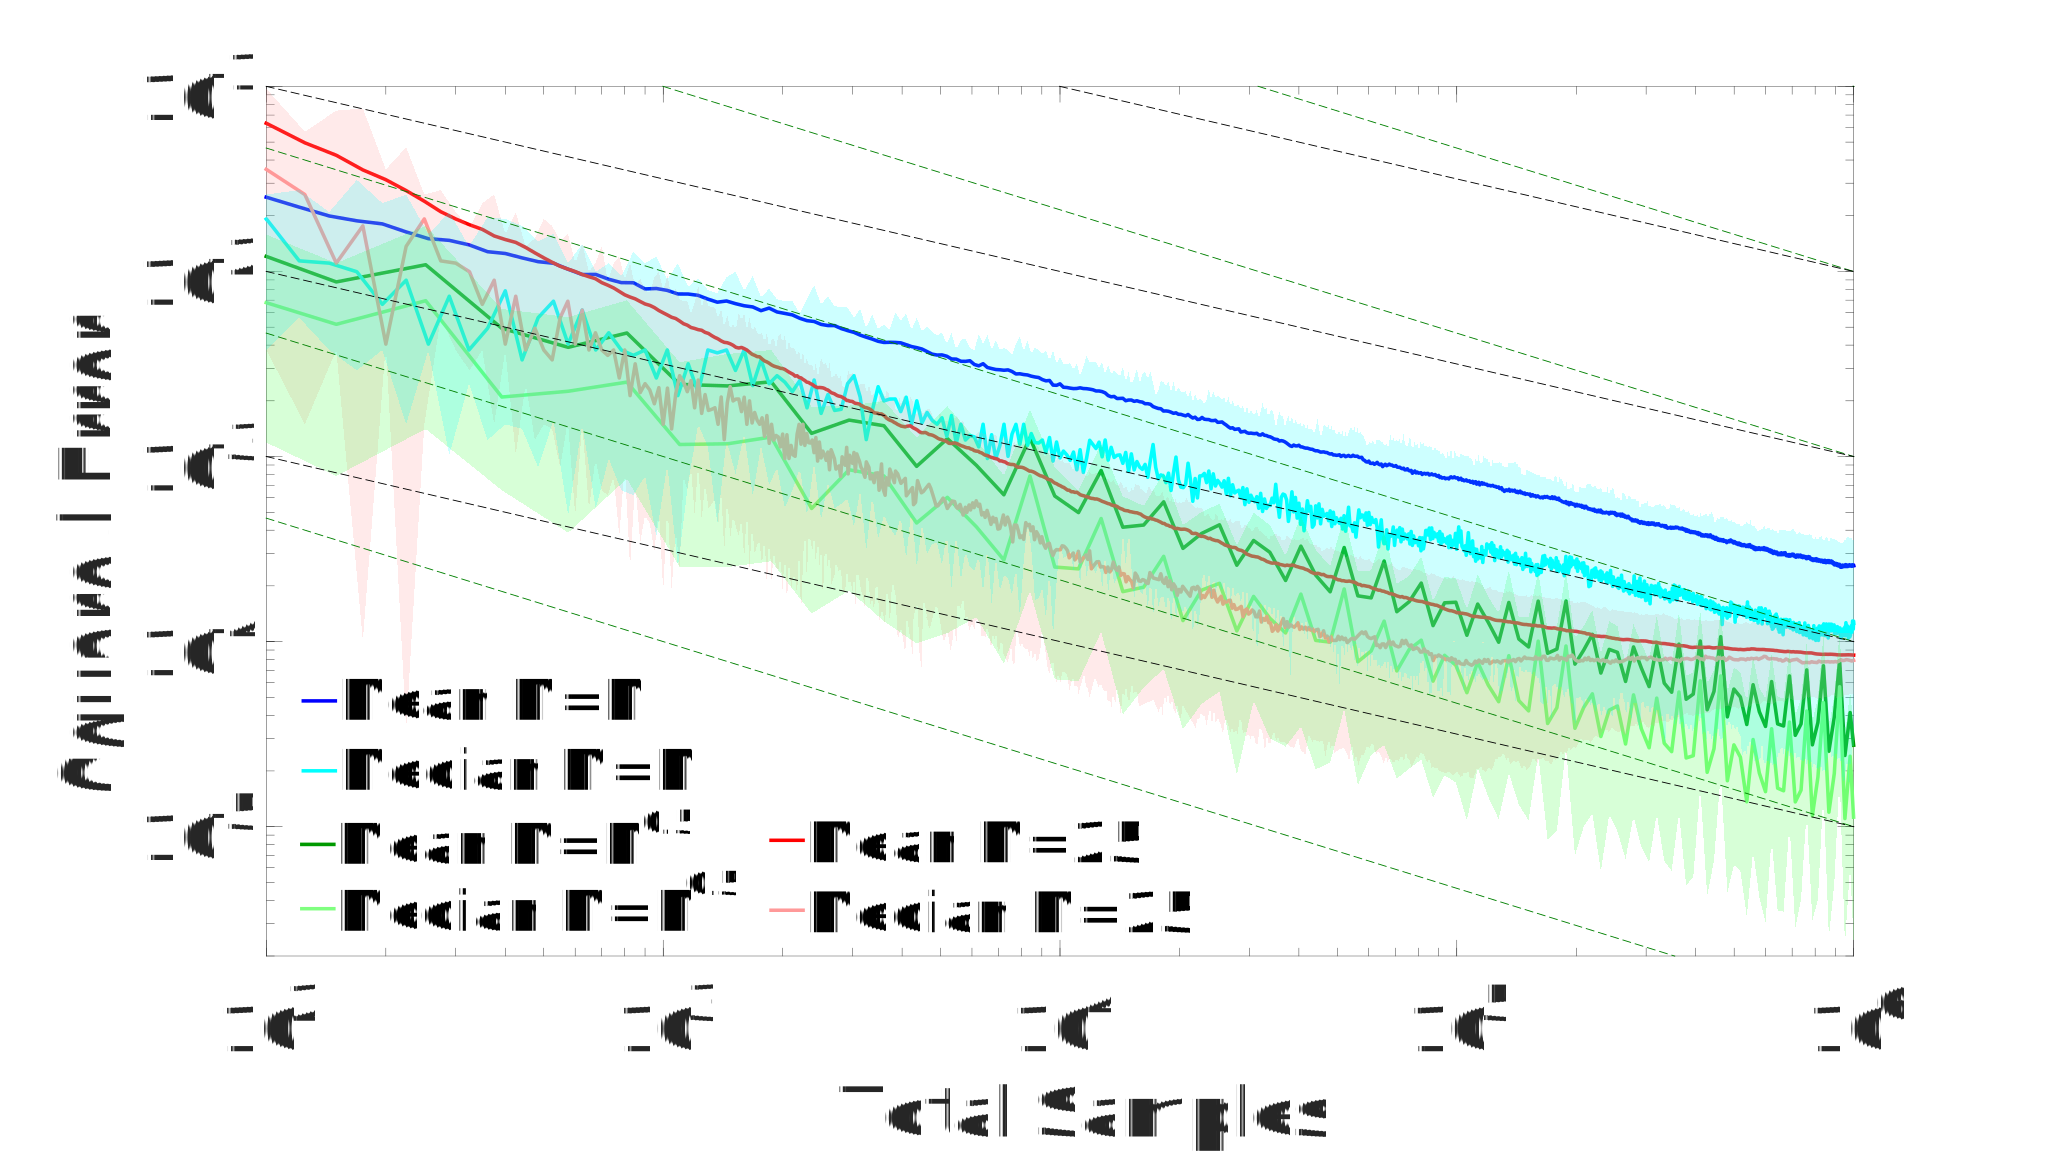
\includegraphics[width=0.49\textwidth,trim={1.5cm 0 3.5cm 0},clip]{canver_conv2}
%	\caption{Convergence of NMC for cancer simulation.
%		A ground truth estimate was calculated
%		using a single run with $M=10^5$ and $N=10^5$.
%		Results are averaged over 1000 independent runs, while shaded regions give the 25\%-75\% quantiles. We
%		see that the theoretical convergence rates are observed in all cases.
%		When $M=\sqrt{N}$ an interesting fluctuation behavior is observed.  
%		Further testing suggests that this originates because the bias of the estimator depends in
%		a fluctuating manner on the value of $M$ as the binary output of $\phi(y,z)$ creates a quantization
%		effect on the possible estimates for $\hat{\gamma}$.  This effect is also observed for the $M=N$ case,
%		but is less pronounced. \label{fig:emperical-conv-cancer} \vspace{-5pt}}
%\end{figure}
%
%The treatment center now wishes to estimate the expected number of patients that will be treated for a given $T_{\mathrm{treat}}$ so that it can minimize this threshold without exceeding its budget.
%To do this, it needs to calculate the expectation of the clinician's decisions to administer 
%treatment, giving the complete nested expectation for calculating the number of treated patients as
%\begin{equation}
%	\label{eq:cancer}
%I(T_{\mathrm{treat}}) = \E_{p(y)} \left[\mathbb{I}\left(\E_{p(z|y)} [\phi(y,z)]>T_{\mathrm{treat}}\right)\right],
%\end{equation}
%where the identity function $\mathbb{I}(\cdot > T_{\mathrm{treat}})$ imposes a non-linear
%mapping, such that conventional Monte Carlo estimation is not possible. Full details on $\phi$, $p(y)$, and $p(z|y)$ are 
%provided in~\cite{rainforth2017pitfalls}.
%
%To verify the convergence rate, we repeat the analysis from Section~\ref{sec:simple} for the problem defined 
%by~\eqref{eq:cancer} at a fixed value of $T_{\mathrm{treat}}=0.35$. 
%The results, shown in Figure~\ref{fig:emperical-conv-cancer}, again verify the theoretical rates. 
%By further testing different values of $T_{\mathrm{treat}}$, we found $T_{\mathrm{treat}} \ge 0.125$ (i.e.
%go ahead with treatment if the probability of success is 0.125 or greater) to be the optimal under the budget.
% !TEX root =  main.tex

\section{Conclusions}

We have introduced a formal framework for nested Monte Carlo (NMC) estimation and shown that
it can be used to yield a consistent estimator for problems that cannot be tackled
with conventional MC alone.  We have demonstrated convergence rates and that NMC
is, in general, biased. We have introduced a number of techniques for converting certain classes
of NMC problems to conventional MC ones, allowing for improved convergence rates on these problems.
We used one of these to derive a new estimator for Bayesian experimental design
with a superior convergence rate to existing schemes.  For problems that do not satisfy these special
cases, we have highlighted the importance of increasing the number of samples in both the inner
and the outer estimators to ensure convergence.  Our results have implications for numerous
applications, for example probabilistic programming, and serve both as an invitation for further inquiry 
and a caveat against careless use.

%We have shown that it is theoretically possible for a nested Monte Carlo scheme to yield a
%consistent estimator, and have quantified the convergence error associated with doing so.
%However, we have also revealed a number of pitfalls that can arise if nesting is applied
%na\"{i}vely, such as the resulting estimator becoming necessarily biased, requiring additional
%assumptions on $f$, being unlikely to converge unless the number of samples used in the inner
%estimator is driven to infinity,
%and is likely to converge at a significantly slower rate than un-nested Monte
%Carlo. These results have implications for applications ranging from experimental design
%to probabilistic programming, and serve both as an invitation for further inquiry and a
%caveat against careless use.

%We have shown that although consistent nested inference is still possible, it is inherently biased, requires Lipshitz continuity, and has a convergence rate that reduces exponentially in the nesting depth.  
%These results have implications for many applications such as experimental design and probabilistic programming.
%For the latter, it shows that when there is only a linear dependence on the nested query, the problem can be unravelled to a single inference, but that otherwise there are additional severe restrictions on the problems that can be solved and the performance that can be achieved.
%When there is only a linear dependence of the outer integration on the nested expectation, the problem can be unravelled to a single inference, therefore, although nested queries in probabilistic programs do increase the scope of models which can be defined, these models have continuity restrictions and only permit MC inference at prohibitively slower convergence rates than ordinary inference.

% !TEX root = ../main.tex

\section{Proofs}
\label{sec:nest:proofs}
% !TEX root =  ../main.tex

\subsection{Proof of Theorem~\ref{the:finite-res} - Convergence Rate for Finite Realisations of $y$}
\label{sec:app:finite-res}

%\begin{theorem}
%	If $f$ is Lipschitz continuous, then the mean squared error of 
%	\[
%	I_N = \sum_{c=1}^C (\hat{P}_N)_c \, (\hat{f}_N)_c
%	\]
%	as an estimator for $I$ converges at rate $O(1/N)$.
%\end{theorem}
\thefiniteres*

\begin{proof}
	Denote
	$P_c = P(y = y_c)$ and
	$f_c = f(y_c, \gamma(y_c))$
	noting that as the $y_c$ are fixed values, so are $P_c$ and $f_c$.
	Then, Minkowski's inequality allows us to bound the mean squared error as
	\begin{eqnarray*}
		\E\left[(I_N - I)^2\right] = \norm{I_N - I}_2^2
		\leq \left(\sum_{c=1}^C W_c \right)^2 \quad \text{where} \quad W_c := \norm{(\hat{P}_N)_c \, (\hat{f}_N)_c - P_c \, f_c}_2.
	\end{eqnarray*}
	Moreover, again by Minkowski, we have $W_c \leq U_c + V_c$
	where 
	\[
	U_c = \norm{(\hat{P}_N)_c \, (\hat{f}_N)_c - (\hat{P}_N)_c \, f_c}_2, \quad
	V_c = \norm{(\hat{P}_N)_c \, f_c - P_c \, f_c}_2.
	\]
	Factoring out $(\hat{P}_N)_c$ in $U_c$ and noting that each $y_n$ and $z_{n,c}$ are sampled independently gives
	\begin{eqnarray*}
		U_c = \sqrt{\E\left[(\hat{P}_N)_c^2 \, \left((\hat{f}_N)_c - f_c\right)^2\right]} 
		= \sqrt{\E\left[(\hat{P}_N)_c^2\right]} \sqrt{\E\left[\left((\hat{f}_N)_c - f_c\right)^2\right]}.
	\end{eqnarray*}
	Using Minkowski's
	inequality, we may write the first right-hand term as
	\begin{eqnarray*}
		\sqrt{\E\left[(\hat{P}_N)_c^2\right]} = \norm{(\hat{P}_N)_c}_2
		&\leq& \frac{1}{N} \sum_{n=1}^N \norm{\mathbbm{1}(y_n = y_c)}_2 \\
		&=&\frac{1}{N} \sum_{n=1}^N \E \left[{\mathbbm{1}(y_n = y_c)}^2\right] 
		= \frac{1}{N} \sum_{n=1}^N P_c
		= P_c.
	\end{eqnarray*}
	For the second term, note that by Lipschitz continuity, we have for some constant $K >
	0$
	\begin{eqnarray*}
		\sqrt{\E\left[\left((\hat{f}_N)_c - f_c\right)^2\right]} = \norm{(\hat{f}_N)_c - f_c}_2 &\leq& 
		K \, \norm{\frac{1}{N} \sum_{n=1}^N \phi(y_c, z_{n,c}) - \gamma(y_c)}_2  \\	
		&=& K \cdot O(1/\sqrt{N}) 
		= O(1/\sqrt{N}),
	\end{eqnarray*}
	since $\frac{1}{N} \sum_{n=1}^N \phi(y_c, z_{n,c})$ is a Monte Carlo estimator for
	$\gamma(y_c)$. Altogether then, we have that
	\[
	U_c = P_c \cdot O(1 / \sqrt{N}) = O(1 / \sqrt{N}).
	\]
	We can also factor out $f_c$ in $V_c$ to obtain
	\[
	V_c = |f_c| \cdot \norm{(\hat{P}_N)_c - P_c}_2 = |f_c| \cdot O(1/\sqrt{N}) = O(1/\sqrt{N}),
	\]
	since $(\hat{P}_N)_c$ is a Monte Carlo estimator for $P_c$.
	Now by noting that 
	$(A+B)^2 \le 2(A^2+B^2)$
	for any $A, B \in \mathbb{R}$, an inductive arguments shows that 
	\[
	\left(\sum_{\ell=1}^L A_\ell\right)^2 \leq 2^{\lceil \log_2 L \rceil} \sum_{\ell=1}^L A_\ell^2
	\]
	for all $A_1, \cdots, A_L \in \mathbb{R}$.  We can now show that
	our asymptotic bounds for $U_c$ and $V_c$ entail that our overall mean squared
	error satisfies
	\begin{eqnarray}
	\E\left[(I_N - I)^2\right] &\leq& 2^{\lceil \log_2 C \rceil} \sum_{c=1}^C W_c^2 \label{eq:square-inequal-1} \notag
	\leq 2^{\lceil \log_2 C \rceil} \sum_{c=1}^C (U_c + V_c)^2 \notag
	\leq 2^{\lceil \log_2 C \rceil + 1} \sum_{c=1}^C U_c^2 + V_c^2 \label{eq:square-inequal-2} \notag \\
	&=& 2^{\lceil \log_2 C \rceil + 1} \sum_{c=1}^C O(1/N) + O(1/N) \notag
	= O(1/N), \notag
	\end{eqnarray}
	as desired.
\end{proof}
% !TEX root =  ../main.tex

\subsection{Products of Expectations}
\label{sec:app-prod}

\theprod*

\begin{proof}
	Consider fixed sizes of nested sample sets, $\{M_\ell\}_{\ell = 1:L}$.
	For each $y \in \mathcal{Y}$ and 
        \[
                x = \{\{z_{\ell,m}'\}_{m=1:M_{\ell}}\}_{\ell=1:L} \in \mathcal{X} 
                = \mathcal{Z}_1^{M_{1}} \otimes \dots \otimes \mathcal{Z}_L^{M_L},
        \]
	define 
	\[
	\eta(y,x) = f\left(y,\prod_{\ell=1}^{L} \frac{1}{M_{\ell}} \sum_{m_{\ell}=1}^{M_{\ell}} \psi_{\ell}(y,z_{\ell,m}')\right).
	\]
	Now, $I_{N} = \frac{1}{N} \sum_{n=1}^{N} \eta(y_n,x_n)$ is a standard
	MC estimator on the space $\mathcal{Y} \otimes \mathcal{X}$. Thus,
	$I_{N} \asto \mathbb{E}[I_{N}]$ with convergence properties and rate as per standard MC.  
	We finish the proof by showing that $\mathbb{E}[I_{N}]=I$ when $f$ is linear:
	\begin{align*}
	\displaybreak[0]
	\mathbb{E}[I_{N}] &= \mathbb{E} \left[\frac{1}{N} \sum_{n=1}^N f\left(y_n,\prod_{\ell=1}^{L} \frac{1}{M_{\ell}}  \sum_{m=1}^{M_{\ell}} \psi_{\ell}(y_n,z_{n,\ell,m}') \right)\right] \\
	\displaybreak[0]
	&= \mathbb{E} \left[f\left(y_1,\prod_{\ell=1}^{L} \frac{1}{M_{\ell}}  \sum_{m=1}^{M_{\ell}} \psi_{\ell}(y_1,z_{1,\ell,m}') \right)\right] \\
	\displaybreak[0]
	&= \mathbb{E}\left[ \mathbb{E}\left[ f\left( y_1,\prod_{\ell=1}^{L} \frac{1}{M_{\ell}}  \sum_{m=1}^{M_{\ell}} \psi_{\ell}(y_1,z_{1,\ell,m}')\right) \middle| y_1 \right]\right],
	\end{align*}
	now using the linearity of $f$
	\begin{align*}
	\displaybreak[0]
	\phantom{\mathbb{E}[I_{N}]} &= \mathbb{E}\left[ f\left( y_1,\mathbb{E}\left[ \prod_{\ell=1}^{L} \frac{1}{M_{\ell}}  \sum_{m=1}^{M_{\ell}} \psi_{\ell}(y_1,z_{1,\ell,m}') \middle| y_1 \right] \right) \right],
	\end{align*}
	and using the fact that terms for different $\ell$ are by construction independent
	\begin{align*}
	\displaybreak[0]
	\phantom{\mathbb{E}[I_{N}]} 
	&= \mathbb{E}\left[ f\left( y_1, \prod_{\ell=1}^L\mathbb{E}\left[\frac{1}{M_{\ell}}  \sum_{m=1}^{M_{\ell}} \psi_{\ell}(y_1,z_{1,\ell,m}') \middle| y_1 \right] \right) \right] \\
	\displaybreak[0]
	&= \mathbb{E}\left[ f\left( y_1, \prod_{\ell=1}^{L}\mathbb{E}\left[\psi_{\ell}(y_1,z'_{1,\ell,1}) \middle| y_1 \right]\right)\right] \\
	&= I,
	\end{align*}
	as required.
\end{proof}

% !TEX root =  ../main.tex

\subsection{Proof of Theorem~\ref{the:Rate} - Convergence Rate}
\label{sec:app:rate_single}

\theRate*

\begin{proof}
	Though the proof follows directly from Theorem~\ref{the:Repeat}, we also provide the following proof 
	for this simplified case as a stepping stone to aid in understanding the more general proof.
	
	Using Minkowski's inequality, we can bound the mean squared error of $I_{N,M}$ by
	\begin{align} \label{eq:mse-bound-app}\begin{split}
	\E[(I-I_{N,M})^2] &= \norm{I - I_{N,M}}_2^2 \leq {U}^2 + {V}^2 + 2 U V \leq 2\left(U^2 + V^2\right)
	\end{split}
	\end{align}
	\begin{eqnarray*}
		\text{where} \quad U = \norm{I - \frac{1}{N} \sum_{n=1}^N f(y_n, \gamma(y_n))}_2
		\quad \text{and} \quad
		V = \norm{\frac{1}{N} \sum_{n=1}^N f(y_n, \gamma(y_n)) - I_{N,M}}_2.
	\end{eqnarray*}
	We see immediately that $U = O\left(1 / \sqrt{N}\right)$, since $\frac{1}{N} \sum_{n=1}^N
	f(y_n, \gamma(y_n))$ is a MC estimator for $I$, noting our assumption that
	$f(y_n, \gamma(y_n)) \in L^2$. For the second term,
	\begin{eqnarray*}
		V &=& \norm{\frac{1}{N} \sum_{n=1}^N f(y_n, (\hat{\gamma}_M)_n) - f(y_n, \gamma(y_n))}_2 \\
		&\leq& \frac{1}{N} \sum_{n=1}^{N} \norm{f(y_n, (\hat{\gamma}_M)_n) - f(y_n,
			\gamma(y_n))}_2
		\leq \frac{1}{N} \sum_{n=1}^N K \norm{(\hat{\gamma}_M)_n - \gamma(y_n)}_2 \\
	\end{eqnarray*}
	where $K$ is a fixed constant, again by Minkowski and using the assumption that $f$ is
	Lipschitz. We can rewrite
	\[
	\norm{(\hat{\gamma}_M)_n - \gamma(y_n)}_2^2
	= \E \left[ \E \left[ ((\hat{\gamma}_M)_n - \gamma(y_n))^2 \middle| y_n \right]\right].
	\]
	by the tower property of conditional expectation, and note that
	\begin{align*}
	\E &\left[ ((\hat{\gamma}_M)_n - \gamma(y_n))^2 \middle| y_n \right]
	= \var\left(\frac{1}{M} \sum_{m=1}^M \phi(y_n, z_{n,m}) \middle| y_n \right) 
	= \frac{1}{M} \var\left(\phi(y_n, z_{n,1}) \middle| y_n \right)
	%    &=& \E_{y_n \sim p(y)} \left[ O(1/M) \right] \\
	%    &=& O(1/M),
	\end{align*}
	since each $z_{n,m}$ is i.i.d. and conditionally independent given $y_n$. As
	such
	\begin{align*}
	\norm{(\hat{\gamma}_M)_n - \gamma(y_n)}_2^2
	&= \frac{1}{M} \, \E \left[ \var \left(\phi(y_n, z_{n,1}) \middle| y_n \right)\right] 
	= O(1/M),
	\end{align*}
	noting that $\E \left[ \var \left(\phi(y_n, z_{n,1}) \middle| y_n \right)\right]$ is a
	finite constant by our assumption that $\phi(y_n, z_{n,m}) \in L^2$. Consequently,
	\[
	V \leq \frac{NK}{N} O\left(1/\sqrt{M}\right) = O\left(1/\sqrt{M}\right).
	\]
	Substituting these bounds for $U$ and $V$ in \eqref{eq:mse-bound-app} gives
	\begin{align*}
	\norm{I - I_{N,M}}_2^2
	&\leq 2\left(O\left(1/\sqrt{N}\right)^2 + O\left(1/\sqrt{M}\right)^2\right) 
	= O\left(1/N + 1/M\right)
	\end{align*}
	as desired.
\end{proof}
% !TEX root =  main.tex

\subsection{`Almost Almost Sure'' Convergence}
\label{sec:app:consistent}

\theConsistent*

\begin{proof}
	For all $N, M$, we have by the triangle inequality that
		\begin{align*}
	\left|I_{N,M} - I\right| \leq V_{N,M} + U_N, &\quad \text{where} \\
		V_{N,M} = \left|\frac{1}{N} \sum_{n=1}^N f(y_n, \gamma(y_n)) - I_{N,M} \right| 
		\quad \text{and}& \quad
		U_N = \left|I - \frac{1}{N} \sum_{n=1}^N f(y_n, \gamma(y_n)) \right|.
	\end{align*}
	A second application of the triangle inequality then allows us to write
	\[
    V_{N,M} \leq \frac{1}{N} \sum_{n=1}^N (\epsilon_M)_n
	\]
	where we recall that $(\epsilon_M)_n = |f(y_n, \gamma(y_n)) - f(y_n, \hat{\gamma}_n)|$.
	Now, for all fixed $M$, each $(\epsilon_M)_n$ is i.i.d. Furthermore, since
        $\E
	\left[(\epsilon_M)_1\right] \to 0$ as $M \to \infty$ by our assumption and 
	$(\epsilon_M)_n$ is nonnegative, there exists some $L \in \N$
	such that $\E\left[\left|(\epsilon_M)_n \right|\right] < \infty$ for all $M \geq L$.
	Consequently, the strong law of large numbers means that as $N \to \infty$ then for all $M \geq L$
	\begin{align}
	\label{eq:epas}
	\frac{1}{N} \sum_{n=1}^N (\epsilon_M)_n \asto \E\left[(\epsilon_M)_1\right].
	\end{align}      
        For any fixed $\delta > 0$ then by repeatedly applying Egorov's theorem to each $M \geq L$,
        we can find a sequence of events 
        \[
                B_{L}, B_{L+1}, B_{L+2}, \ldots
        \]
        such that for every $M \geq L$,
        \[
                \mathbb{P}(B_{M}) < \frac{\delta}{4} \cdot \frac{1}{2^{M-L}}
        \]
        and outside of $B_{M}$, the sequence $\frac{1}{N} \sum_{n=1}^N (\epsilon_M)_n$
        converges \emph{uniformly} to $\E\left[(\epsilon_M)_1\right]$. 
        This uniform convergence (as opposed to just the piecewise convergence implied
        by~\eqref{eq:epas}) now guarantees that we can define some function
        $\tau^1_\delta : \N \to \N$ such that 
	\begin{align}
	\label{eq:ombo}
                \left|\frac{1}{M'} \sum_{n=1}^{M'} (\epsilon_M)_n(\omega) - \E\left[(\epsilon_M)_1\right]\right| < \frac{1}{M} 
        \end{align}
        for all $M \geq L$, $M' \geq \tau^1_\delta(M)$, and $\omega \not\in B_M$, remembering that $\omega$ is
        a point in our sample space.  We further have that~\eqref{eq:ombo} holds for all 
        $M \geq M_0$, $M' \geq \tau^1_\delta(M)$, and $\omega \not\in B_\delta := \bigcup_{M \geq L} B_M$.
%        Such a $\tau^1_\delta$ exists
%        because of the uniform convergence guarantee that we just mentioned. 
%        Defining 
%        \[
%                B_\delta := \bigcup_{M \geq L} B_M,
%        \]
%        then~\eqref{eq:ombo} hold for all $M \geq M_0$, $M' \geq \tau^1_\delta(M)$, and $\omega \not\in B_\delta$.
        Consequently, for all such $M$, $M'$ and $\omega$,
        \begin{equation} 
                \label{eqn:almostsure:1}
                V_{M',M}(\omega)
                \leq
                \frac{1}{M'} \sum_{n=1}^{M'} (\epsilon_M)_n(\omega) 
                < 
                \frac{1}{M} + \E\left[(\epsilon_M)_1\right],
        \end{equation}
        while we also have
        \begin{equation} 
                \label{eqn:almostsure:2}
                \mathbb{P}(B_\delta) 
                %=\mathbb{P}\left(\bigcup_{M \geq L} B_M\right)
                \leq 
                \sum_{M \geq L} \mathbb{P}\left(B_M\right)
                < \sum_{M \geq L} \frac{\delta}{4} \cdot \frac{1}{2^{M-L}}
                = \frac{\delta}{2}.
        \end{equation}
      To complete the proof, we must remove the dependence of $U_N$ on $N$ as well. This is
	straightforward once we observe that $U_N \asto 0$ as $N \to \infty$ by the strong law of 
        large numbers. So, by Egorov's theorem again, there exists an event $C_\delta$ such that
        \begin{equation} 
                \label{eqn:almostsure:3}
                \mathbb{P}(C_\delta) < \frac{\delta}{2}
        \end{equation}
        and outside of $C_\delta$, the sequence $U_N$ converges uniformly to $0$. This uniform convergence,
        in turn, ensures the existence of a function $\tau^2_\delta : \N \to \N$ such that
        \begin{equation} 
                \label{eqn:almostsure:4}
                U_{M'}(\omega) < \frac{1}{M} 
        \end{equation}
        for all $M \in \N$, $M' \geq \tau^2_\delta(M)$, and $\omega \not\in C_\delta$.
	
        We can now define $\tau_\delta(M) = \max(\tau^1_\delta(M), \tau^2_\delta(M))$, and 
        $A_\delta = B_\delta \cup C_\delta$. By inequalities in \eqref{eqn:almostsure:2}
        and \eqref{eqn:almostsure:3},
        \[ 
                \mathbb{P}(A_\delta) \leq \mathbb{P}(B_\delta) + \mathbb{P}(C_\delta) < \delta.  
        \] 
        Also, by the inequalities in \eqref{eqn:almostsure:1} and \eqref{eqn:almostsure:4},
	\[ 
                \left|I - I_{\tau_\delta(M),M}(\omega)\right| 
                \leq
                V_{\tau_\delta(M),M}(\omega) 
                +
                U_{\tau_\delta(M)}(\omega) 
                \leq 
                \frac{1}{M} + \frac{1}{M} + \E\left[(\epsilon_M)_1\right]
	\]
        for all $M \geq L$ and $\omega \notin A_\delta$. Since $\E\left[(\epsilon_M)_1\right] \to 0$, we have here that 
        $I_{\tau_\delta(M),M}(\omega) \to I$ as desired.
\end{proof}

% !TEX root =  main.tex
%
%\section{Proof of Theorem~\ref{the:Repeat} - Convergence for Repeated Nesting (Simple From)}
%\label{sec:app:repeat}
%
%Below we provide a proof of Theorem~\ref{the:Repeat} from the main paper.  We note that this covers 
%Theorem~\ref{the:Rate} as a special case and is itself covered by Theorem~\ref{the:biggie} which
%is more general and also provides the constants associated with the bound.  
%Although only the third Theorem and proof is technically necessary, we provide all three 
%in the interest of exposition, with each theorem and proof somewhat more involved than the last.  
%The proofs for Theorems~\ref{the:Rate} 
%and~\ref{the:Repeat} are based on the same techniques so the former provides a stepping stone
%for understanding the latter.  Theorem~\ref{the:biggie} has a completely different proof (based
%on bias-variance decompositions) but is particularly involved.  The early two are thus provided
%to give insight without requiring understanding of this more challenging proof.
%
%\theRepeat*
%
%\begin{proof}
%  To establish this claim, we show that for \emph{all} $0 \leq k \leq D$, the mean squared
%  error
%  \begin{equation} \label{eq:mse-rate-goal}
%    \norm{\gamma_k\left(y^{(0:k-1)}\right) - I_k\left(y^{(0:k-1)}\right)}^2_2
%    = O\left(\sum_{\ell=k}^D \frac{1}{N_\ell}\right).
%  \end{equation}
%  Our theorem corresponds to the case that $k = 0$.
%  
%  We proceed by applying Minkowski's inequality, which allows us to bound
%  \[
%    \norm{\gamma_k\left(y^{(0:k-1)}\right) - I_k\left(y^{(0:k-1)}\right)}_2^2
%    \leq U_k^2 + V_k^2 + 2U_kV_k \leq 2(U_k^2 + V_k^2),
%  \]
%  where
%  \begin{eqnarray*}
%    U_k &=& \norm{\gamma_k\left(y^{(0:k-1)}\right) - J_k\left(y^{(0:k-1)}\right)}_2 \\
%    V_k &=& \norm{J_k\left(y^{(0:k-1)}\right) - I_k\left(y^{(0:k-1)}\right)}_2
%  \end{eqnarray*}
%  and we define
%  \[
%    J_k\left(y^{(0:k-1)}\right) = \frac{1}{N_k} \sum_{n=1}^{N_k} f_k\left(y^{(0:k-1)}, y^{(k)}_n, \gamma_{k+1}\left(y^{(0:k-1)}, y^{(k)}_n\right)\right)
%  \]
%  for $0 \leq k < D$, and
%  \[
%    J_D\left(y^{(0:D-1)}\right) = I_D\left(y^{(0:D-1)}\right).
%  \]
%  Intuitively, $J_k\left(y^{(0:k-1)}\right)$ corresponds to applying an MC approximation
%  to $\gamma_k\left(y^{(0:k-1)}\right)$ only to the outermost expectation, and exactly
%  computing the expectations nested within.
%
%  We show below that
%  \begin{equation} \label{eq:mse-Uk-goal}
%    U_k^2 = O\left(\frac{1}{N_k}\right)
%  \end{equation}
%  for all $k$, which, since $V_D = 0$, establishes \eqref{eq:mse-rate-goal} for the case
%  $k = D$. For the remaining $k$, we note that
%  \begin{eqnarray*}
%    V_k &\leq& \frac{1}{N_k} \sum_{n=1}^{N_k}
%      \bigg\Vert f_k\left(y^{(0:k-1)}, y^{(k)}_n, \gamma_{k+1}\left(y^{(0:k-1)}, y^{(k)}_n\right)\right) \\
%    &\phantom{\leq}& \phantom{\frac{1}{N_k} \sum_{n=1}^{N_k}\bigg\Vert} 
%    - f_k\left(y^{(0:k-1)}, y^{(k)}_n, I_{k+1}\left(y^{(0:k-1)}, y^{(k)}_n\right)\right) \bigg\Vert_2 \\
%    &\leq& \frac{K}{N_k} \sum_{n=1}^{N_k} \norm{\gamma_{k+1}\left(y^{(0:k-1)}, y^{(k)}_n\right) - I_{k+1}\left(y^{(0:k-1)}, y^{(k)}_n\right)}_2,
%  \end{eqnarray*}
%  for some $K > 0$, by Minkowski's inequality and using the assumption that $f_k$ is
%  Lipschitz. Since the $y_n^{(k)} \sim p(y^{(k)}|y^{(0:k-1)})$ are i.i.d., we can rewrite
%  this inequality as
%  \[
%    V_k \leq K \norm{\gamma_{k+1}\left(y^{(0:k)}\right) - I_{k+1}\left(y^{(0:k)}\right)}_2
%  \]
%  so that
%  \[
%    V_k^2 \leq K^2 \norm{\gamma_{k+1}\left(y^{(0:k)}\right) - I_{k+1}\left(y^{(0:k)}\right)}_2^2.
%  \]
%  We see that the second term on the right-hand side has the same form as
%  \eqref{eq:mse-rate-goal}, and so recursing on $k$ (until the base case $k = D$) allows
%  us to bound
%  \[
%    V_k^2 \leq K^2 \, O\left(\sum_{\ell=k+1}^N \frac{1}{N_\ell} \right).
%  \]
%  This then yields
%  \[
%    \norm{\gamma_k\left(y^{(0:k-1)}\right) - I_k\left(y^{(0:k-1)}\right)}^2_2
%    \leq 2 \left(O\left(\frac{1}{N_k}\right) + K^2 \, O\left(\sum_{\ell=k+1}^N \frac{1}{N_\ell} \right) \right)
%    = O\left(\sum_{\ell=k}^D \frac{1}{N_\ell}\right)
%  \]
%  as desired.
%
%  It remains to show \eqref{eq:mse-Uk-goal}. To do so, we first observe that
%  \[
%    U_k^2 = \E\left[ \E\left[ \left(\gamma_k\left(y^{(0:k-1)}\right) - J_k\left(y^{(0:k-1)}\right)\right)^2 \middle| y^{(0:k-1)} \right] \right]
%  \]
%  by the tower property of conditional expectation. Now, 
%  \begin{align*}
%    \E\left[ \left(\gamma_k\left(y^{(0:k-1)}\right) - J_k\left(y^{(0:k-1)}\right)\right)^2 \middle| y^{(0:k-1)} \right]
%    &= \var \left[J_k\left(y^{(0:k-1)}\right) \middle| y^{(0:k-1)} \right] \\
%    = \frac{1}{N_k} \var &\left[f_k\left(y^{(0:k)}, \gamma_{k+1}\left(y^{(0:k)}\right)\right) \middle| y^{(0:k-1)} \right]
%  \end{align*}
%  (omitting the $\gamma_{k+1}$ term when $k = D$), since each $y^{(k)}_n$ in
%  $J_k\left(y^{(0:k-1)}\right)$ is conditionally independent given $y^{(0:k-1)}$.
%  Consequently,
%  \[
%    U_k^2 = \frac{1}{N_k} \E \left[ \var \left[f_k\left(y^{(0:k)}, \gamma_{k+1}\left(y^{(0:k)}\right)\right) \middle| y^{(0:k-1)} \right] \right]
%    = O\left(\frac{1}{N_k}\right),
%  \]
%  noting that $\E \left[ \var \left[f_k\left(y^{(0:k)},
%  \gamma_{k+1}\left(y^{(0:k)}\right)\right) \middle| y^{(0:k-1)} \right] \right]$ is a
%  finite constant by our assumption that $f_k\left(y^{(0:k)},
%  \gamma_{k+1}\left(y^{(0:k)}\right)\right) \in L^2$ (and where once again we omit the
%  $\gamma_{k+1}$ terms when $k = D$).
%\end{proof}

\subsection{General Convergence Rate}
\label{sec:app:repeat}
%
%Below we provide a proof of Theorem~\ref{the:Repeat} from the main paper.  We note that this covers 
%Theorem~\ref{the:Rate} as a special case.  A separate proof for Theorem~\ref{the:Rate} was provided in
%Appendix~\ref{sec:app:rate_single}.  This may make easier reading on a first pass as 
%it is substantially less involved that the following, more general case.

\theRepeat*
\begin{proof}
As this is a long and involved proof, we start by defining a number of useful terms that will be 
used throughout.  Unless otherwise stated, these definitions hold for all $k \in \left\{0,\dots,D\right\}$.
Note that most of these terms implicitly depend on the number of
samples $N_0,N_1,\dots,N_D$.  However, $s_k$, $\zeta_{d,k}$, and $\varsigma_k$ do not
and are thus constants for a particular problem.
\begin{align}
\intertext{$E_k \left(y^{(0:k-1)}\right)$ is the MSE of the estimator at depth $k$ given $y^{(0:k-1)}$}
E_k \left(y^{(0:k-1)}\right) &:= \E \left[\left(I_{k}\left(y^{(0:k-1)}\right)-
\gamma_{k}\left(y^{(0:k-1)}\right)\right)^2 \middle| y^{(0:k-1)}\right]
\displaybreak[0] \\
\intertext{$\bar{f}_{k} \left(y^{(0:k-1)}\right)$ is the expected value of the estimate at depth
	$k$, or equivalently the expected function output using the estimate of the layer below}
\begin{split}
\bar{f}_{k} \left(y^{(0:k-1)}\right) &:=\E\left[I_{k}\left(y^{(0:k-1)}\right) \middle| y^{(0:k-1)}\right] \;\; \forall k\in\{1,\dots,D-1\} \\
&=\E\left[f_k\left(y^{(0:k)},I_{k+1}\left(y^{(0:k)}\right)\right)
\middle|  y^{(0:k-1)}\right] 
\end{split}
\displaybreak[0] \\ 
\intertext{$v_k^2 \left(y^{(0:k-1)} \right)$ is the variance of the estimator at depth $k$}
    \begin{split}
    	v_k^2 \left(y^{(0:k-1)} \right) &:= 
    	\text{Var}\left[I_{k}\left(y^{(0:k-1)}\right) \middle| y^{(0:k-1)}\right] \\
    	&= \E\left[\left(I_{k}\left(y^{(0:k-1)}\right)- \bar{f}_k 
    	\left(y^{(0:k-1)}\right) \right)^2 \middle| y^{(0:k-1)}\right]
    \end{split}
\displaybreak[0]   \\ 
\intertext{$\beta_k \left(y^{(0:k-1)} \right)$ is the bias of the estimator at depth $k$}
   \begin{split}
   	\label{eq:bias-def}
   	\beta_k \left(y^{(0:k-1)} \right) &:= 
   	\E  \left[I_{k}\left(y^{(0:k-1)}\right)-
   	\gamma_{k}\left(y^{(0:k-1)}\right) \middle| y^{(0:k-1)}\right] \\
   	&=\bar{f}_{k} \left(y^{(0:k-1)}\right)-\gamma_{k}\left(y^{(0:k-1)}\right) \\
   	&=
   	\E \left[f_k\left(y^{(0:k)}, I_{k+1}\left(y^{(0:k)}\right)\right)
   	- f_k\left(y^{(0:k)}, \gamma_{k+1}\left(y^{(0:k)}\right)\right)
   	\middle|  y^{(0:k-1)} \right]
   \end{split}
\displaybreak[0] \\ 
\intertext{$s_k^2 \left(y^{(0:k-1)}\right)$ is the variance at depth $k$ of the true function output}
s_k^2 \left(y^{(0:k-1)}\right) &:= \E \left[\left(f_k\left(y^{(0:k)},\gamma_{k+1}
\left(y^{(0:k)}\right) \right)-\gamma_k\left(y^{(0:k-1)}\right)\right)^2 \middle|
y^{(0:k-1)}	\right]
\\ \displaybreak[0]
s_D^2 \left(y^{(0:D-1)}\right) &:= \E \left[\left(f_D\left(y^{(0:D)}\right)-\gamma_D\left(y^{(0:D)}\right)\right)^2 \middle| y^{(0:D-1)}	\right]
\\
\intertext{$\zeta_{d,k}^2\left(y^{(0:k-1)}\right)$ is expectation of $s_d^2 \left(y^{(0:d-1)}\right)$ over 
	$y^{(k:d-1)}$}
\begin{split}
	\zeta_{d,k}^2\left(y^{(0:k-1)}\right) &:= 
	\E \left[ s_{d}^2 \left(y^{(0:d-1)}\right) \middle|
	y^{(0:k-1)}\right] \\
	&=\E \left[\left(f_d\left(y^{(0:d)},\gamma_{d+1}
	\left(y^{(0:d)}\right) \right)-\gamma_d\left(y^{(0:d-1)}\right)\right)^2 \middle|
	y^{(0:k-1)}	\right]
\end{split}
\displaybreak[0] \\
\intertext{$\varsigma_{k}^2 $ is expectation of $s_k^2 \left(y^{(0:k-1)}\right)$
	over all $y^{(0:k-1)}$}
\varsigma_{k}^2  
&:=\zeta_{k,0}^2=\E \left[\left(f_k\left(y^{(0:k)},\gamma_{k+1}
\left(y^{(0:k)}\right) \right)-\gamma_k\left(y^{(0:k-1)}\right)\right)^2\right]
 \displaybreak[0] \\
 \intertext{$A_k \left(y^{(0:k-1)}\right)$ is the MSE in the function output from
 	using the estimate of the next layer, rather than the true value $\gamma_{k+1}\left(y^{(0:k)}\right)$,
 	we fix $A_D:=0$}
A_k \left(y^{(0:k-1)}\right):=& \E \left[\left(f_k\left(y^{(0:k)}, I_{k+1}\left(y^{(0:k)}\right)\right)
- f_k\left(y^{(0:k)}, \gamma_{k+1}\left(y^{(0:k)}\right)\right)\right)^2
\middle|  y^{(0:k-1)} \right] 
%\\\displaybreak[0]
%A_D &:=0 
\displaybreak[0]\\
 \intertext{$\sigma_k^2 \left(y^{(0:k-1)}\right)$
 	is the variance in the function output from using the estimate of the next layer,
 	we fix $\sigma_D^2 \left(y^{0:D-1}\right) := s_D^2 \left(y^{0:D-1}\right)$ }
 \begin{split}
 \sigma_k^2 \left(y^{(0:k-1)}\right) &:= 
 \text{Var}\left[f_k\left(y^{(0:k)},I_{k+1}\left(y^{(0:k)}\right)\right) \middle| y^{(0:k-1)}\right] \\
 &= \E\left[\left(f_k\left(y^{(0:k)},I_{k+1}\left(y^{(0:k)}\right)\right)
 - \bar{f}_k 
 \left(y^{(0:k-1)}\right) \right)^2 \middle| y^{(0:k-1)}\right]
 \end{split}
\displaybreak[0]  \\ 
 \intertext{$\omega_k\left(y^{(0:k-1)} \right)$ is the expectation over $y^{(k)}$ of the MSE for the next layer,
 	we fix $\omega_D \left(y^{(0:D-1)}\right) := 0$}
      \begin{split}
      \omega_k\left(y^{(0:k-1)} \right) &:=  \E \left[E_{k+1} 
      \left(y^{(0:k)}\right) \middle|  y^{(0:k-1)} \right] \\
      &=\E \left[
      \left(I_{k+1}\left(y^{(0:k)}\right) - \gamma_{k+1}\left(y^{(0:k)}\right)\right)^2
      \middle|  y^{(0:k-1)} \right] 
      \end{split}
  \displaybreak[0]
 \\
  \intertext{$\lambda_k \left(y^{(0:k-1)} \right)$ is the expectation over $y^{(k)}$ of the magnitude of the bias for the next layer,
  	we fix $\lambda_D \left(y^{(0:D-1)}\right) := 0$ and note that $\lambda_{D-1} \left(y^{(0:D-2)}\right) := 0$ also
  	as the innermost layer is an unbiased}
    \begin{split}
   \lambda_k \left(y^{(0:k-1)} \right) &:= \E \left[\left|\beta_{k+1} 
   \left(y^{(0:k)}\right) \right| \Bigg|   y^{(0:k-1)} \right]\\
   &=
   \E \left[ \left|\E \left[
   \left(I_{k+1}\left(y^{(0:k)}\right) - \gamma_{k+1}\left(y^{(0:k)}\right)\right)
   \middle|  y^{(0:k)} \right] \right| \Bigg|  y^{(0:k-1)} \right]
   \end{split}
\end{align}

\vspace{5pt}
\noindent\textbf{\large Lipschitz Continuous Case}
\vspace{5pt}

\noindent Given these definitions, we start by breaking the error down into a variance and bias term.  
Using the standard bias-variance decomposition we have
\begin{align}
E_k \left(y^{(0:k-1)}\right) &= \E \left[\left(I_{k}\left(y^{(0:k-1)}\right)-
\gamma_{k}\left(y^{(0:k-1)}\right)\right)^2 \middle| y^{(0:k-1)}\right]
\nonumber \\
&=v_k^2 \left(y^{(0:k-1)} \right)
+\left(\beta_k \left(y^{(0:k-1)} \right)\right)^2 \label{eq:bias-var-decomp}
\end{align}
It is immediately clear from its definition in \eqref{eq:bias-def} that the bias term
$\left(\beta_k \left(y^{(0:k-1)} \right)\right)^2$ is independent of 
$N_0$.  On the other hand, we will show later that the
dominant components of the variance term for large $N_{0:D}$ depend only
on $N_0$.  We can thus think of increasing $N_0$ as reducing the variance of
the estimator and increasing $N_{1:D}$ as reducing the bias.

We first consider the variance term
\begin{align*}
v_k^2 \left(y^{(0:k-1)} \right) &= \E \left[\left(
\frac{1}{N_k} \sum_{n=1}^{N_k} f_k\left(y^{(0:k)}_n, I_{k+1}\left(y^{(0:k)}_n\right)\right)-
\bar{f}_k 
\left(y^{(0:k-1)}\right) \right)^2 \middle| y^{(0:k-1)}\right]   \displaybreak[0] \\
&=\frac{1}{N_k} \E \left[\left(
f_k\left(y^{(0:k)}, I_{k+1}\left(y^{(0:k)}\right)\right)-
\bar{f}_k 
\left(y^{(0:k-1)}\right) \right)^2 \middle| y^{(0:k-1)}\right]
\end{align*}
with the equality following because the $y_n^{(0:k)}$ being drawn i.i.d. and the
expectation of each
$f_k\left(y^{(0:k)}, I_{k+1}\left(y^{(0:k)}\right)\right)$ equaling $\bar{f}_k 
\left(y^{(0:k-1)}\right)$ means that all the cross terms are zero.
%&= \E \left[\frac{1}{N_k^2} \sum_{n=1}^{N_k} \left(
% f_k\left(y^{(0:k)}_n, I_{k+1}\left(y^{(0:k)}_n\right)\right)-
%\bar{f}_k 
%\left(y^{(0:k-1)}\right) \right)^2 \middle| y^{(0:k-1)}\right] \\
%&\phantom{=} +\E \left[\frac{1}{N_k^2} \sum_{n=1}^{N_k} \sum_{m=1, m\neq n}^{N_k}\left(
%f_k\left(y^{(0:k)}_n, I_{k+1}\left(y^{(0:k)}_n\right)\right)-
%\bar{f}_k 
%\left(y^{(0:k-1)}\right) \right) \right.\\
%&\quad\quad\quad\quad\quad\quad
%\cdot\left(
%f_k\left(y^{(0:k)}_m, I_{k+1}\left(y^{(0:k)}_m\right)\right)-
%\bar{f}_k 
%\left(y^{(0:k-1)}\right) \right)
% \Bigg| y^{(0:k-1)}\Bigg]
%\end{align*}
%Now noting that each $y_n^{(0:k)}$ are drawn i.i.d., the cross terms are
%independent and the distribution is the same for each $m$ and $n$
% and so we have
%\begin{align*}
%v_k^2 \left(y^{(0:k-1)} \right) &= 
%\frac{1}{N_k} \E \left[\left(
%f_k\left(y^{(0:k)}, I_{k+1}\left(y^{(0:k)}\right)\right)-
%\bar{f}_k 
%\left(y^{(0:k-1)}\right) \right)^2 \middle| y^{(0:k-1)}\right]\\
%&\phantom{=}+\frac{N_k-1}{N_k}
%\left(\E \left[
%f_k\left(y^{(0:k)}, I_{k+1}\left(y^{(0:k)}\right)\right)-
%\bar{f}_k 
%\left(y^{(0:k-1)}\right)\middle| y^{(0:k-1)}\right]\right)^2,
%\end{align*}
%where the second term is zero by the definition of $\bar{f}_k$ and so
By the definition of $\sigma_k^2$ we now have
\begin{align}
	\label{eq:lln}
v_k^2 \left(y^{(0:k-1)} \right)  &= \frac{\sigma_k^2 \left(y^{(0:k-1)} \right)}{N_k}.
\end{align}
By using Minkowski's inequality and the definition of $A_k$ it also follows that
\begin{align}
	\begin{split}
\sigma_k & \left(y^{(0:k-1)} \right) \le 
 \\
&\left(A_k \left(y^{(0:k-1)}\right)\right)^{\frac{1}{2}}+
\left(\E \left[\left(
f_k\left(y^{(0:k)}, \gamma_{k+1}\left(y^{(0:k)}\right)\right)
-\bar{f}_k\left(y^{(0:k-1)}\right)\right)^2 \middle| y^{(0:k-1)} \right] \right)^{\frac{1}{2}}.\label{eq:sigle1}
\end{split}
\end{align}
Using a bias-variance decomposition on the second term above and noting that 
$s_k^2 \left(y^{(0:k-1)} \right)$ and $\bar{f}_k\left(y^{(0:k-1)}\right)-\beta_k \left(y^{(0:k-1)} \right)$
are respectively the variance and expectation of $f_k\left(y^{(0:k)}, \gamma_{k+1}\left(y^{(0:k)}\right)\right)$,
%	and by substituting $\bar{f}_k=\gamma_k\left(y^{(0:k-1)}\right)-\beta_k \left(y^{(0:k-1)} \right)$,
%expanding the square, and noting that 
%$\E \left[f_k\left(y^{(0:k)},\gamma_{k+1}
%\left(y^{(0:k)}\right) \right)-\gamma_k\left(y^{(0:k-1)}\right) \middle| y^{(0:k-1)} \right]=0$ 
we can rearrange the right-hand size of~\eqref{eq:sigle1} to give
%&=
%\left(A_k \left(y^{(0:k-1)}\right)\right)^{\frac{1}{2}} +
%\left( \E \left[\left(f_k\left(y^{(0:k)},\gamma_{k+1}
%\left(y^{(0:k)}\right) \right)-\gamma_k\left(y^{(0:k-1)}\right)+\beta_k \left(y^{(0:k-1)} \right)\right)^2 \middle|
%y^{(0:k-1)}	\right]\right)^{\frac{1}{2}} \nonumber \\
\begin{align}
\sigma_k \left(y^{(0:k-1)} \right) &\le\left(A_k \left(y^{(0:k-1)}\right)\right)^{\frac{1}{2}}
+\left(s_k^2 \left(y^{(0:k-1)} \right) +
\left(\beta_k \left(y^{(0:k-1)} \right)\right)^2 
 \right)^{\frac{1}{2}}. \label{eq:sigma_bound}
\end{align}
Here $s_k^2$ is independent of the number of samples used at any level of the estimate,
while $A_k$ and $\beta_k^2$ are independent of $N_d \; \forall d\le k$.
Now by Jensen's inequality, we have that
\begin{align}
\label{eq:AleB}
\left(\beta_k \left(y^{(0:k-1)}\right)\right)^2 \le
A_k \left(y^{(0:k-1)}\right)
\end{align}
noting that the only difference in the definition of $\left(\beta_k \left(y^{(0:k-1)}\right)\right)^2$
and $A_k \left(y^{(0:k-1)}\right)$ is
whether the squaring occurs inside or outside the expectation.
Therefore, presuming that $A_k$
does not increase with $N_d  \; \forall d>k$, neither will $\sigma_k^2 \left(y^{(0:k-1)} \right)$, and so
the variance term will converge to zero with rate $O(1/N_k)$.  
Further, if ${A_k}\rightarrow 0$ as $N_{k+1},\dots,N_D \rightarrow \infty$,
then for a large number of inner samples $\sigma_k^2 \rightarrow s_k^2$ and thus we will have
$ v_k^2 \left(y^{(0:k-1)} \right) \le \frac{s_k^2}{N_k} +
O\left(\epsilon\right)$ where $O\left(\epsilon\right)$ represents higher order
terms that are dominated in the limit $N_k,\dots,N_D \rightarrow \infty$.
Provided this holds, we will also, therefore, have that
\begin{align}
\label{eq:E_decomp}
E_k \left(y^{(0:k-1)}\right) 
=\frac{\sigma_k^2 \left(y^{(0:k-1)}\right)}{N_k}+ \beta_k^2 \left(y^{(0:k-1)} \right)
&=\frac{s_k^2 \left(y^{(0:k-1)}\right)}{N_k}+ \beta_k^2 \left(y^{(0:k-1)} \right) +O(\epsilon).
\end{align}

We now show that Lipschitz continuity is sufficient for ${A_k}\rightarrow0$ and derive a
concrete bound on the variance by bounding ${A_k}$.  We found that there was no
noticeably tighter bound to be found for $A_k$ using the continuity assumption and
therefore this result will be used for both cases \eqref{eq:bound-lip} 
and~\eqref{eq:bound-cont}.
By definition of Lipschitz continuity,
we have that
\begin{align}
\left(A_k \left(y^{(0:k-1)}\right)\right)^{\frac{1}{2}} &\le
\left(\E \left[K_k^2 \left(I_{k+1}\left(y^{(0:k)}\right)-
 \gamma_{k+1}\left(y^{(0:k)}\right)\right)^2\middle| y^{(0:k-1)}
 \right] \right)^{\frac{1}{2}} \nonumber \\
 &= K_k \left(\omega_k \left(y^{(0:k-1)}\right)\right)^{\frac{1}{2}}
\end{align}
where we remember that $\omega_k \left(y^{(0:k-1)}\right) 
=\E \left[E_{k+1} 
\left(y^{(0:k)}\right) \middle|  y^{(0:k-1)} \right]$ is the expected MSE
of the next level estimator.  Once we also have an expression for the 
bias, we will thus be able to use this bound on $A_k$ along with~\eqref{eq:bias-var-decomp},~\eqref{eq:lln},
and~\eqref{eq:sigma_bound} to inductively derive a bound on the error.

For the case where we only assume Lipschitz continuity then we will simply
use the bound on the bias given by~\eqref{eq:AleB} leading to
\begin{align}
&E_k \left(y^{(0:k-1)}\right) 
\le \frac{\sigma_k^2 \left(y^{(0:k-1)}\right)}{N_k} + A_k \left(y^{(0:k-1)}\right). \\
&\le \frac{s_k^2 \left(y^{(0:k-1)}\right) +
2A_k \left(y^{(0:k-1)}\right)
+2\left(A_k \left(y^{(0:k-1)}\right)\right)^{\frac{1}{2}}
\left(s_k^2 \left(y^{(0:k-1)}\right) + A_k \left(y^{(0:k-1)}\right)\right)^{\frac{1}{2}}}
{N_k} \nonumber\\
&\phantom{\le\le} +A_k \left(y^{(0:k-1)}\right)\nonumber\\
&= \frac{s_k^2 \left(y^{(0:k-1)}\right) +
	2K_k^2 \omega_k \left(y^{(0:k-1)}\right)}{N_k} +K_k^2 \omega_k \left(y^{(0:k-1)}\right)\nonumber\\
&\phantom{==} 	+\frac{2K_k\left(\omega_k \left(y^{(0:k-1)}\right)\right)^{\frac{1}{2}}
\left(s_k^2 \left(y^{(0:k-1)}\right) +  K_k^2 \omega_k \left(y^{(0:k-1)}\right)\right)^{\frac{1}{2}}}
{N_k}\nonumber \displaybreak[0]\\
\begin{split}
&\le \frac{s_k^2 \left(y^{(0:k-1)}\right) +
	4 K_k^2 \omega_k \left(y^{(0:k-1)}\right)
	+2 K_k \left(\omega_k \left(y^{(0:k-1)}\right)\right)^{\frac{1}{2}}
	s_k \left(y^{(0:k-1)}\right)}{N_k}\\
&\phantom{\le\le} +K_k^2 \omega_k \left(y^{(0:k-1)}\right)
\label{eq:general-bound-lip}
\end{split}
\end{align}
which fully defines a bound on conditional the variance of one layer given the mean squared error of the layer below.
In particular as $\omega_D \left(y^{(0:D-1)}\right) = 0$ we now have
\[
E_D \left(y^{(0:D-1)}\right) \le \frac{s_D^2 \left(y^{(0:D-1)}\right)}{N_D} = 
\frac{\E \left[\left(f_D\left(y^{(0:D)}\right)-\gamma_D\left(y^{(0:D)}\right)\right)^2 \middle| y^{(0:D-1)}	\right]}{N_D}
\]
which is the standard error for Monte Carlo convergence.  
We
further have 
\[
\omega_{D-1} \left(y^{(0:D-2)}\right) = 
\E \left[E_{D} 
\left(y^{(0:D-1)}\right) \middle|  y^{(0:D-2)} \right]
=
\frac{\zeta^2_{D,D-1}
	\left(y^{(0:D-2)}\right) }{N_D}.
\]
and thus
\begin{align}
\begin{split}
E_{D-1} &\left(y^{(0:D-2)}\right) \le  \frac{s_{D-1}^2 \left(y^{(0:D-2)}\right)}{N_{D-1}} +
	\frac{4 K_{D-1}^2 \zeta^2_{D,D-1}
		\left(y^{(0:D-2)}\right)}{N_D N_{D-1}} \\
\quad \quad &	+ \frac{2 K_{D-1}s_{D-1} \left(y^{(0:D-2)}\right)
		\zeta_{D,D-1}
		\left(y^{(0:D-2)}\right)}{N_{D-1} \sqrt{N_D}}
+\frac{K_{D-1}^2 \zeta^2_{D,D-1}\left(y^{(0:D-2)}\right)}{N_D}.
\end{split}
\end{align}
This leads to the following result for the single nesting case
\begin{align}
E_0 \le \frac{\varsigma^2_0}{N_0}+\frac{4 K_{0}^2 \varsigma_1^2}{N_0 N_{1}}
+\frac{2 K_{0}\varsigma_{0} \varsigma_1}{N_{0} \sqrt{N_1}}+\frac{K_0 ^2 \varsigma_1^2}{N_1}
\end{align}
$\approx \frac{\varsigma^2_0}{N_0}+\frac{K_0 ^2 \varsigma_1^2}{N_1} = O\left(\frac{1}{N_0}+\frac{1}{N_1}\right)$
where the approximation becomes exact as $N_0,N_1 \rightarrow \infty$.
Note that there is no $O\left(\epsilon\right)$ term as this bound is exact
in the finite sample case.

Things quickly get messy for double nesting and beyond so we will
ignore non-dominant terms in the limit $N_0,\dots,N_D \rightarrow \infty$
and resort to using $O(\epsilon)$ for these instead. 
We first note that removing dominated terms from~\eqref{eq:general-bound-lip} gives
\begin{align}
	\label{eq:Eklip}
E_k \left(y^{(0:k-1)}\right) \le 
\frac{s_k^2}{N_k} + K_k^2 \omega_k \left(y^{(0:k-1)}\right) + O(\epsilon)
\end{align}
as $s_k^2$ does not decrease with increasing $N_{k+1:D}$ whereas the other
terms do.  We therefore also have
\begin{align}
\omega_k \left(y^{(0:k-1)}\right) &= \E \left[E_{k+1} 
\left(y^{(0:k)}\right) \middle|  y^{(0:k-1)} \right] \nonumber \\ &\le \E \left[ \frac{s_{k+1}^2\left(y^{(0:k)}\right)}
{N_{k+1}} + K^2_{k+1} \omega_{k+1} \left(y^{(0:k)}\right) \middle|
y^{(0:k-1)}\right] + O(\epsilon) \label{eq:omega-bound}
\end{align}
and therefore by recursively substituting~\eqref{eq:omega-bound} into itself
we have
\begin{align}
	\label{eq:Komega}
	K_k^2\omega_k \left(y^{(0:k-1)}\right) &\le
	\sum_{d=k+1}^{D} \frac{\left(\prod_{\ell=k}^{d-1} K_{\ell}^2\right)
		\E \left[ s_{d}^2 \left(y^{(0:d-1)}\right) \middle|
		y^{(0:k-1)}\right]}{N_{d}}+ O(\epsilon).
\end{align}
Now noting that $\zeta_{d,k}^2\left(y^{(0:k-1)}\right) =
\E \left[ s_{d}^2 \left(y^{(0:d-1)}\right) \middle| y^{(0:k-1)}\right]$, substituting
\eqref{eq:Komega} back into~\eqref{eq:Eklip} gives
\begin{align}
E_k \left(y^{(0:k-1)}\right) 
%&\le  \frac{s_k^2\left(y^{(0:k-1)}\right)}{N_k} +
%\sum_{d=k+1}^{D} \frac{\left(\prod_{\ell=k}^{d-1} K_{\ell}^2\right)
%	\E \left[ s_{d}^2 \left(y^{(0:d-1)}\right) \middle|
%	y^{(0:k-1)}\right]}{N_{d}}+ O(\epsilon) \\
&= \frac{s_k^2\left(y^{(0:k-1)}\right)}{N_k} +
\sum_{d=k+1}^{D} \frac{\left(\prod_{\ell=k}^{d-1} K_{\ell}^2\right)
	\zeta_{d,k}^2\left(y^{(0:k-1)}\right)}{N_{d}}+ O(\epsilon).
\label{eq:final-lip-bound}
\end{align}
By definition we have that
$\zeta_{0,0}^2 = s_0^2 =\varsigma_0^2$ and $\zeta_{d,0}^2 = \varsigma_d^2$ and
as~\eqref{eq:final-lip-bound} holds in the case $k=0$, 
the mean squared error of the overall estimator is as follows
\begin{align}
\E \left[\left(I_0-\gamma_0\right)^2\right] 
= E_0 \le 
\frac{\varsigma_{0}^2}{N_0} +
\sum_{k=1}^{D} \frac{\left(\prod_{\ell=0}^{k-1} K_{\ell}^2\right)
	\varsigma_{k}^2}{N_{k}}+ O(\epsilon)
\end{align}
and we have the desired result for the Lipschitz case.

\vspace{15pt}
\noindent\textbf{\large Continuously Differentiable Case}
\vspace{5pt}

\noindent We now revisit the bound for the bias in the continuously differentiable case to
show that a tighter overall bound can be found.  We first remember that
\[
\beta_k \left(y^{(0:k-1)} \right) =
\E \left[f_k\left(y^{(0:k)}, I_{k+1}\left(y^{(0:k)}\right)\right)
- f_k\left(y^{(0:k)}, \gamma_{k+1}\left(y^{(0:k)}\right)\right)
\middle|  y^{(0:k-1)} \right].
\]
Taylor's theorem implies that for any continuously differentiable $f_k$ we can write
\begin{align}
	\begin{split}
f_k&\left(y^{(0:k)}, I_{k+1}\left(y^{(0:k)}\right)\right)
	- f_k\left(y^{(0:k)}, \gamma_{k+1}\left(y^{(0:k)}\right)\right) \\
	&\quad\quad\quad\quad= \frac{\partial f_k \left(y^{(0:k)},\gamma_{k+1}(y^{(0:k)})\right)}{\partial \gamma_{k+1}}
		\left(I_{k+1}\left(y^{(0:k)}\right) - \gamma_{k+1}\left(y^{(0:k)}\right)\right) \\
	&\quad\quad\quad\quad\phantom{=}+\frac{1}{2}
	\frac{\partial f_k^{2} \left(y^{(0:k)},\gamma_{k+1}(y^{(0:k)})\right)}{\partial \gamma_{k+1}^{2}}
	\left(I_{k+1}\left(y^{(0:k)}\right) - \gamma_{k+1}\left(y^{(0:k)}\right)\right)^{2} \\
	&\quad\quad\quad\quad\phantom{=}+h_3\left(I_{k+1}\left(y^{(0:k)}\right) \right) 
	\left(I_{k+1}\left(y^{(0:k)}\right) - \gamma_{k+1}\left(y^{(0:k)}\right)\right)^{3}
	\end{split}
\end{align}
where $\lim_{x\rightarrow\gamma_{k+1}\left(y^{(0:k)}\right)}h_3(x)=0$.  Consequently, the
last term is $O\left(\left(I_{k+1}\left(y^{(0:k)}\right) - \gamma_{k+1}\left(y^{(0:k)}\right)\right)^{3}\right)$
and so will diminish in magnitude faster than the first two terms provided that the derivatives are
bounded, which is guaranteed by our assumptions.  We will thus use $O(\epsilon)$ for this term and note that
it is dominated in the limit.

Now defining
\begin{align*}
	%\delta_{1,k} &= \E \left[\frac{\partial f_k \left(y^{(0:k)},\gamma_{k+1}(y^{(0:k)})\right)}{\partial \gamma_{k+1}}
	%\left(I_{k+1}\left(y^{(0:k)}\right) - \gamma_{k+1}\left(y^{(0:k)}\right)\right)
	%\middle|  y^{(0:k-1)} \right] \\
	\delta_{\ell,k} &= \E \left[ \frac{\partial f_k^{\ell} \left(y^{(0:k)},\gamma_{k+1}(y^{(0:k)})\right)}{\partial \gamma_{k+1}^{\ell}}
	\left(I_{k+1}\left(y^{(0:k)}\right) - \gamma_{k+1}\left(y^{(0:k)}\right)\right)^{\ell}
	\middle|  y^{(0:k-1)} \right] 
\end{align*}
then we have
\begin{align*}
	\beta_k^2 \left(y^{(0:k-1)} \right)
	=&\delta_{1,k}^2+\frac{\delta_{2,k}^2}{4}+\delta_{1,k}\delta_{2,k} +O(\epsilon).
\end{align*}
%We now use a Taylor expansion for $f_k\left(y^{(0:k)}, I_{k+1}\left(y^{(0:k)}\right)\right)$ about the point
%$f_k\left(y^{(0:k)}, \gamma_{k+1}\left(y^{(0:k)}\right)\right)$
%as follows where all derivatives are with respect to the second input.  First we
%define
%\begin{align*}
%%\delta_{1,k} &= \E \left[\frac{\partial f_k \left(y^{(0:k)},\gamma_{k+1}(y^{(0:k)})\right)}{\partial \gamma_{k+1}}
%%\left(I_{k+1}\left(y^{(0:k)}\right) - \gamma_{k+1}\left(y^{(0:k)}\right)\right)
%%\middle|  y^{(0:k-1)} \right] \\
%\delta_{\ell,k} &= \E \left[ \frac{\partial f_k^{\ell} \left(y^{(0:k)},\gamma_{k+1}(y^{(0:k)})\right)}{\partial \gamma_{k+1}^{\ell}}
%\left(I_{k+1}\left(y^{(0:k)}\right) - \gamma_{k+1}\left(y^{(0:k)}\right)\right)^{\ell}
%\middle|  y^{(0:k-1)} \right] 
%\end{align*}
%then we have from the Taylor expansion
%\begin{align*}
%\beta_k^2 \left(y^{(0:k-1)} \right) =& 
%\left(\E \left[f_k\left(y^{(0:k)}, \gamma_{k+1}\left(y^{(0:k)}\right)\right)
%\middle|  y^{(0:k-1)} \right]+
%\delta_{1,k}+\frac{\delta_{2,k}}{2}
%+O(\epsilon) \right.\\
%&\left.\quad-\E \left[f_k\left(y^{(0:k)}, \gamma_{k+1}\left(y^{(0:k)}\right)\right)
%\middle|  y^{(0:k-1)} \right]\right)^2 \\
%=&\delta_{1,k}^2+\frac{\delta_{2,k}^2}{4}+\delta_{1,k}\delta_{2,k} +O(\epsilon).
%\end{align*}
By using the tower property we further have that
\begin{align*}
\delta_{\ell,k} &= \E \left[ \E \left[\frac{\partial f_k^{\ell} \left(y^{(0:k)},\gamma_{k+1}(y^{(0:k)})\right)}{\partial \gamma_{k+1}^{\ell}}
\left(I_{k+1}\left(y^{(0:k)}\right) - \gamma_{k+1}\left(y^{(0:k)}\right)\right)^{\ell}
\middle|  y^{(0:k)} \right] \middle|  y^{(0:k-1)} \right] \displaybreak[0]\\
&= \E \left[ \frac{\partial f_k^{\ell} \left(y^{(0:k)},\gamma_{k+1}(y^{(0:k)})\right)}{\partial \gamma_{k+1}^{\ell}} \E \left[
\left(I_{k+1}\left(y^{(0:k)}\right) - \gamma_{k+1}\left(y^{(0:k)}\right)\right)^{\ell}
\middle|  y^{(0:k)} \right] \middle|  y^{(0:k-1)} \right] \displaybreak[0]\\
&\le \E \left[ \left|\frac{\partial f_k^{\ell} \left(y^{(0:k)},\gamma_{k+1}(y^{(0:k)})\right)}{\partial \gamma_{k+1}^{\ell}} \right| 
\left|\E \left[
\left(I_{k+1}\left(y^{(0:k)}\right) - \gamma_{k+1}\left(y^{(0:k)}\right)\right)^{\ell}
\middle|  y^{(0:k)} \right] \right| \; \middle|  y^{(0:k-1)} \right]  \displaybreak[0]\\
&\le \left(\sup_{y^{(0)}} \left|
\frac{\partial^{\ell} f_k \left(y^{(0:k)},\gamma_{k+1}(y^{(0:k)})\right)}{\partial \gamma^{\ell}_{k+1}} \right| \right)\\
&\quad\quad \cdot \E \left[\left| \E \left[
\left(I_{k+1}\left(y^{(0:k)}\right) - \gamma_{k+1}\left(y^{(0:k)}\right)\right)^{\ell}
\bigg| y^{(0:k)} \right]
\right| \; \Bigg| y^{(0:k-1)} \right].
\end{align*}
Now for the particular cases of $\ell=1$ and $\ell=2$ then the derivative terms where 
defined in the theorem and the expectations correspond respectively to our definitions of $\lambda_k$ and $\omega_k$
giving
\begin{align*}
\delta_{1,k} &\le  K_k \lambda_k\left(y^{(0:k-1)} \right) \\
\delta_{2,k} &\le C_k \omega_k\left(y^{(0:k-1)} \right)
\end{align*}
and therefore
%\begin{align}
%\beta_k^2 \left(y^{(0:k-1)} \right)  \le 
%K_k^2 \omega_k\left(y^{(0:k-1)} \right) + 
%\frac{C_k^2}{4} \omega_k^2\left(y^{(0:k-1)} \right)
%+K_k C_k \omega_k^{\frac{3}{2}}\left(y^{(0:k-1)} \right)+O(\epsilon)
%\end{align}
\begin{align}
\beta_k^2 \left(y^{(0:k-1)} \right)  &\le K_k^2 \lambda_k^2 \left(y^{(0:k-1)} \right) +\frac{C_k^2}{4} \omega_k^2\left(y^{(0:k-1)} \right) \nonumber\\&\phantom{\le\le}+K_k\; C_k \; \lambda_k \left(y^{(0:k-1)} \right) \omega_k \left(y^{(0:k-1)} \right) + O(\epsilon) \nonumber\\
&=\left(K_k \lambda_k \left(y^{(0:k-1)} \right) +
\frac{C_k}{2} \omega_k\left(y^{(0:k-1)} \right) \right)^2+O(\epsilon). \label{eq:beta-k-cont}
\end{align}

Remembering~\eqref{eq:E_decomp}
%$E_k \left(y^{(0:k-1)}\right) 
%= \frac{\sigma_k^2 \left(y^{(0:k-1)}\right)}{N_k} + \beta_k^2 \left(y^{(0:k-1)}\right)$,
we can recursively define the error bound in the same manner as the Lipschitz case.  We can immediately see that,
as $\beta_D =0$ without any nesting, we recover the bound from the Lipschitz case for the inner most estimator as expected.  
As the innermost estimator is unbiased we also have
$\lambda_{D-1} \left(y^{(0:D-2)} \right)=0$ and so
\begin{align*}
\beta_{D-1}^2 \left(y^{(0:D-2)} \right) &\le \frac{C_{D-1}^2}{4} \omega^2_{D-1} \left(y^{(0:D-2)}\right) + O(\epsilon) \\
&\le \frac{C_{D-1}^2}{4} 
\left(\E \left[\frac{s_D^2\left(y^{(0:D-1)}\right)}{N_D}
\middle|  y^{(0:D-2)} \right]\right)^2+ O(\epsilon) \\
&= \frac{C_{D-1}^2 \; \zeta^4_{D,D-1}
	\left(y^{(0:D-2)}\right) }{4N_D^2}+ O(\epsilon).
\end{align*}
Using the full expansion of $\sigma_{D-1}^2 \left(y^{(0:D-2)}\right)$
derived in the Lipschitz case and the exact form of~\eqref{eq:E_decomp} we have
\begin{align}
\begin{split}
& E_{D-1}\left(y^{(0:D-2)}\right) \le  \frac{s_{D-1}^2 \left(y^{(0:D-2)}\right)}{N_{D-1}} +
\frac{4K_{D-1}^2 \zeta^2_{D,D-1}
	\left(y^{(0:D-2)}\right)}{N_D N_{D-1}} \\
&\quad \quad + \frac{2 K_{D-1}s_{D-1} \left(y^{(0:D-2)}\right)
	\zeta_{D,D-1}
	\left(y^{(0:D-2)}\right)}{N_{D-1} \sqrt{N_D}}
+\frac{C_{D-1}^2 \; \zeta^4_{D,D-1}
	\left(y^{(0:D-2)}\right) }{4N_D^2}+ O(\epsilon).
\end{split}
\end{align}
Therefore for the single nesting case, we now have
\begin{align}
E_0 \le \frac{\varsigma^2_0}{N_0}+\frac{4 K_{0}^2 \varsigma_1^2}{N_0 N_{1}}
+\frac{2 K_{0}\varsigma_{0} \varsigma_1}{N_{0} \sqrt{N_1}}+\frac{C_0 ^2 \varsigma_1^4}{4 N_1^2}
+ O\left(\frac{1}{N_1^3}\right)
\end{align}
$\approx \frac{\varsigma^2_0}{N_0}+\frac{C_0 ^2 \varsigma_1^4}{4 N_1^2} = O\left(\frac{1}{N_0}+\frac{1}{N_1^2}\right)$
where again the approximation becomes tight when $N_0,N_1 \rightarrow \infty$.
Here we have used the fact that the only $O(\epsilon)$ term comes from the Taylor expansion.
In this case, we have $\delta_{1,D-1}=0$ and so we have
\begin{align*}
O(\epsilon)&=O\left(\delta_{2,D-1}\E \left[
\left(I_{1}\left(y^{(0)}\right) - \gamma_{1}\left(y^{(0)}\right)\right)^{3}\middle| y^{(0)}\right]\right) \\
&=O\left(\frac{1}{N_1}\E \left[
\left(\frac{1}{N_1}\sum_{n=1}^{N_1} f_1\left(y^{(0:1)}_n\right)- \E \left[f_1\left(y^{(0:1)}\right) \middle| y^{(0)}\right]\right)^{3}\middle| y^{(0)}\right]\right)
\end{align*}
which can easily be shown to be $O\left(1/N_1^3\right)$ as required.
\\
%as $\E \left[
%\left(I_{1}\left(y^{(0)}\right) - \gamma_{1}\left(y^{(0)}\right)\right)^4
%\right]=O\left(\frac{1}{N_1^{2}}\right)$.  Therefore $\frac{\delta_{2,k} \delta_{3,k}}{3}
%=O\left(\frac{1}{N_1^{5/2}}\right)$ which confirms that the $O(\epsilon)$ term is
%asymptotically negligible as required and allows us to better characterize the
%bound in the single nesting case as we have
%\begin{align}
%E_0 \le \frac{\varsigma^2_0}{N_0}+\frac{4 K_{0}^2 \varsigma_1^2}{N_0 N_{1}}
%+\frac{2 K_{0}\varsigma_{0} \varsigma_1}{N_{0} \sqrt{N_1}}+\frac{C_0 ^2 \varsigma_1^4}{4 N_1^2}
%+ O\left(\frac{1}{N_1^{5/2}}\right).
%\end{align}

\noindent Returning to calculating the bound for the repeated nesting case then by 
substituting~\eqref{eq:beta-k-cont} into~\eqref{eq:E_decomp} we have more generally
\begin{align}
	E_k \left(y^{(0:k-1)}\right) 
	&\le \frac{s_k^2 \left(y^{(0:k-1)}\right)}{N_k}+ \left(K_k \lambda_k \left(y^{(0:k-1)} \right) +
	\frac{C_k}{2} \omega_k\left(y^{(0:k-1)} \right) \right)^2+O(\epsilon). \label{eq:Ekcont}
	\end{align}
Now remembering that
$\omega_k \left(y^{(0:k-1)}\right) = \E \left[E_{k+1} 
\left(y^{(0:k)}\right) \middle|  y^{(0:k-1)} \right] $ from~\eqref{eq:E_decomp} we have
\begin{align}
	\omega_k\left(y^{(0:k-1)} \right) &= \E \left[\frac{s_{k+1}^2 \left(y^{(0:k)}\right)}{N_{k+1}} + \beta^2_{k+1} 
	\left(y^{(0:k)}\right) \middle|  y^{(0:k-1)} \right] + O(\epsilon) \nonumber \\
	&= \frac{\zeta_{k+1,k}^2}{N_{k+1}}+\E \left[\beta^2_{k+1} 
	\left(y^{(0:k)}\right) \middle|  y^{(0:k-1)} \right] + O(\epsilon).  \label{eq:omega}
\end{align}
We also have that except at $k=D-1$ and $k=D$ (for which both $\lambda_k$ and $\beta_{k+1}$ are zero), then
\[
\lambda_k\left(y^{(0:k-1)} \right) = \E \left[\left|\beta_{k+1} 
\left(y^{(0:k)}\right) \right| \Bigg|  y^{(0:k)}\right] \gg
\E \left[\beta^2_{k+1} 
\left(y^{(0:k)}\right) \middle|  y^{(0:k-1)} \right]
\]
for sufficiently large $N_{k+1},\dots,N_D$.
This means that when we substitute~\eqref{eq:omega} into~\eqref{eq:Ekcont},
the second term in \eqref{eq:omega} becomes dominated giving
\begin{align}
	E_k \left(y^{(0:k-1)}\right) 
	\le\frac{s_k^2 \left(y^{(0:k-1)}\right)}{N_k}
	+\left(K_k \lambda_k \left(y^{(0:k-1)}\right) 
	+\frac{C_k \zeta_{k+1,k}^2}{2 N_{k+1}}\right)^2 + O(\epsilon). \label{eq:E_k_for_sub}
\end{align}
%\noindent Returning to calculating the bound for the repeated nesting case, we have
%\begin{align}
%\omega_k\left(y^{(0:k-1)} \right) &= \E \left[\frac{s_{k+1}^2 \left(y^{(0:k)}\right)}{N_{k+1}} + \beta^2_{k+1} 
%\left(y^{(0:k)}\right) \middle|  y^{(0:k-1)} \right] + O(\epsilon) \nonumber \\
%&= \frac{\zeta_{k+1,k}^2}{N_{k+1}}+\E \left[\beta^2_{k+1} 
%\left(y^{(0:k)}\right) \middle|  y^{(0:k-1)} \right] + O(\epsilon)  \label{eq:omega}
%\end{align}
%and except at $k=D-1$ and $k=D$ (for which both $\lambda_k$ and $\beta_{k+1}$ are zero), then
%\[
%\lambda_k\left(y^{(0:k-1)} \right) = \E \left[\left|\beta_{k+1} 
%\left(y^{(0:k-1)}\right) \right| \Bigg|  y^{(0:k)}\right] \gg
%\E \left[\beta^2_{k+1} 
%\left(y^{(0:k)}\right) \middle|  y^{(0:k-1)} \right]
%\]
%for sufficiently large $N_{k+1},\dots,N_D$.
% We can therefore ignore the second term in $\omega_k$ as follows.   Starting from~\eqref{eq:E_decomp}
% and substituting in~\eqref{eq:beta-k-cont} we have
% \begin{align}
%  E_k \left(y^{(0:k-1)}\right) 
% &=\frac{s_k^2 \left(y^{(0:k-1)}\right)}{N_k}+ \beta_k^2 \left(y^{(0:k-1)} \right) +O(\epsilon) \nonumber \\
% &\le \frac{s_k^2 \left(y^{(0:k-1)}\right)}{N_k}+ \left(K_k \lambda_k \left(y^{(0:k-1)} \right) +
% \frac{C_k}{2} \omega_k\left(y^{(0:k-1)} \right) \right)^2+O(\epsilon) \nonumber \\
% &= \frac{s_k^2 \left(y^{(0:k-1)}\right)}{N_k}
% +\left(K_k \lambda_k \left(y^{(0:k-1)}\right) 
% +\frac{C_k \zeta_{k+1,k}^2}{2 N_{k+1}}\right)^2 + O(\epsilon). \label{eq:E_k_for_sub}
% \end{align}
%again ignore the higher order terms giving
%\begin{align*}
%& E_k \left(y^{(0:k-1)}\right) 
%=\frac{s_k^2 \left(y^{(0:k-1)}\right)}{N_k} + \beta_k^2 \left(y^{(0:k-1)}\right)
%+ O(\epsilon) \\
%&\quad \quad \le \frac{s_k^2 \left(y^{(0:k-1)}\right)}{N_k} +K_k^2 \lambda_k^2 \left(y^{(0:k-1)} \right) +\frac{C_k^2}{4} \omega_k^2\left(y^{(0:k-1)} \right) \\
%&\quad \quad \quad +K_kC_k \lambda_k \left(y^{(0:k-1)} \right) \omega_k \left(y^{(0:k-1)} \right) + O(\epsilon)
%  \displaybreak[0] \\ 
%&\quad \quad = \frac{s_k^2 \left(y^{(0:k-1)}\right)}{N_k}+K_k^2
% \left(\E \left[\left|\beta_{k+1} 
% \left(y^{(0:k)}\right) \right| \Bigg|  y^{(0:k-1)} \right]\right)^2 \\
% &\quad \quad \quad+\frac{C_k^2}{4} \left( \E \left[\frac{s_{k+1}^2 \left(y^{(0:k)}\right)}{N_{k+1}} + \beta^2_{k+1} 
% \left(y^{(0:k)}\right) \middle|  y^{(0:k-1)} \right]\right)^2 \\
% &\quad \quad \quad+K_kC_k 
% \E \left[\left|\beta_{k+1} 
% \left(y^{(0:k)}\right) \right| \Bigg|   y^{(0:k-1)} \right]
% \E \left[\frac{s_{k+1}^2 \left(y^{(0:k)}\right)}{N_{k+1}} + \beta^2_{k+1} 
% \left(y^{(0:k)}\right) \middle|  y^{(0:k-1)} \right] +O(\epsilon).
%\end{align*}
%We first consider the double nested case for which
%\begin{align*}
% \E \left[\beta^2_{1} 
% \left(y^{(0:1)}\right) \middle|  y^{(0)} \right] \le 
%  C_{1}^2 \E \left[ \omega^2_1 \left(y^{(0)}\right) \middle|  y^{(0)}  \right] + O(\epsilon) 
% &=
% \frac{C_{1}^2 \E \left[ \zeta^4_{2,1}
% 	\left(y^{(0)}\right) \middle|  y^{(0)}  \right]}{4 N_2^2}  + O(\epsilon) \\
% \E \left[\left|\beta_{1} 
% \left(y^{(0:1)}\right) \right| \Bigg|  y^{(0)} \right] \le 
%   C_{1}^2 \E \left[ \left|\omega_1 \left(y^{(0)}\right) \right| \Bigg|  y^{(0)}  \right] + O(\epsilon) 
%   &=
% \frac{C_{1} \E \left[ \zeta^2_{2,1}
% 	\left(y^{(0)}\right) \middle|  y^{(0)}  \right]}{2N_2}  + O(\epsilon) \\
% &=  \frac{C_{1} \varsigma_{2}^2}{2 N_2}  + O(\epsilon)
%\end{align*}
%and thus
%\begin{align*}
%E_0 \le& \frac{s_0^2}{N_0}+\frac{K_0^2 C_{1}^2 \varsigma_{2}^4}{4 N_2^2}+
%\frac{C_0^2\varsigma_1^4}{4 N_1^2}+\frac{C_0^2C_1^2\varsigma_1^2
%	\E \left[ \zeta^4_{2,1}
%	\left(y^{(0)}\right) \middle|  y^{(0)}  \right]}{8N_1N_2^2}+
%\frac{C_0^2C_1^4
%	\left(\E \left[ \zeta^4_{2,1}
%	\left(y^{(0)}\right) \middle|  y^{(0)}  \right]\right)^2}{64 N_2^4} \\
%&+\frac{K_0C_0C_1\varsigma_1^2\varsigma_2^2}{2N_1N_2}
%+\frac{K_0C_0C_1^3\varsigma_2^2 \E \left[ \zeta^4_{2,1}
%	\left(y^{(0)}\right) \middle|  y^{(0)}  \right]}{8N_2^3} +O(\epsilon).
%\end{align*}
%Dropping the higher order terms, we have
%\begin{align*}
%E_0 \le& \frac{s_0^2}{N_0}+\frac{K_0^2 C_{1}^2 \varsigma_{2}^4}{4 N_2^2}+
%\frac{C_0^2\varsigma_1^4}{4 N_1^2}
%+\frac{K_0C_0C_1\varsigma_1^2\varsigma_2^2}{2N_1N_2}+O(\epsilon)
%=\frac{s_0^2}{N_0}+\frac{1}{4}\left(\frac{K_0 C_{1} \varsigma_{2}^2}{N_2}+
%\frac{C_0\varsigma_1^2}{N_1}\right)^2
%+O(\epsilon).
%%\end{align*}
%Now we note that except at $k=D-1$ and $k=D$
%for which they are zero, the
%$ \E \left[\left|\beta_{1} 
%\left(y^{(0:1)}\right) \right| \Bigg|  y^{(0)} \right]$
%terms dominate
% the $ \E \left[\beta_{1} 
% \left(y^{(0:1)}\right)^2 \middle|  y^{(0)} \right]$ terms.
% We can therefore ignore the latter as higher order terms as follows
% \begin{align*}
%& E_k \left(y^{(0:k-1)}\right) 
%=\frac{s_k^2 \left(y^{(0:k-1)}\right)}{N_k}+K_k^2
%\lambda_k^2 \left(y^{(0:k-1)}\right) +\frac{C_k^2}{4 N_{k+1}^2} \left( \E \left[s_{k+1}^2 \left(y^{(0:k)}\right) \middle|  y^{(0:k-1)} \right]\right)^2 \\
% &\quad \quad \quad \quad \quad \quad \phantom{=}+\frac{K_kC_k}{N_{k+1}}
%\lambda_k \left(y^{(0:k-1)}\right) 
% \E \left[s_{k+1}^2 \left(y^{(0:k)}\right)  \middle|  y^{(0:k-1)} \right] +O(\epsilon) \\
% &\quad \quad  = \frac{s_k^2 \left(y^{(0:k-1)}\right)}{N_k}+K_k^2
%\lambda_k^2 \left(y^{(0:k-1)}\right) +\frac{C_k^2 \zeta_{k+1,k}^4}{4 N_{k+1}^2} +\frac{K_kC_k\zeta_{k+1,k}^2}{N_{k+1}}
%\lambda_k \left(y^{(0:k-1)}\right) +O(\epsilon) \\
% &\quad \quad = \frac{s_k^2 \left(y^{(0:k-1)}\right)}{N_k}
% +\left(K_k \lambda_k \left(y^{(0:k-1)}\right) 
% +\frac{C_k \zeta_{k+1,k}^2}{2 N_{k+1}}\right)^2 + O(\epsilon).
% \end{align*}
 Now as $\beta_{k+1}^2 \left(y^{(0:k)}\right) =E_{k+1} 
 \left(y^{(0:k)}\right) -\frac{s_{k+1}^2 \left(y^{(0:k)}\right)}{N_{k+1}}$ we have
 \begin{align*}
  \lambda_k \left(y^{(0:k-1)}\right)  &=
  \E \left[\sqrt{E_{k+1} 
  \left(y^{(0:k)}\right) -\frac{s_{k+1}^2 \left(y^{(0:k)}\right)}{N_{k+1}}}
  \middle|  y^{(0:k-1)}  \right] +O(\epsilon)\\
  \intertext{and substituting in~\eqref{eq:E_k_for_sub} gives}
 \lambda_k \left(y^{(0:k-1)}\right)  &\le \E \left[K_{k+1} \lambda_{k+1} \left(y^{(0:k)}\right) 
  +\frac{C_{k+1} \zeta_{k+2,k+1}^2}{2 N_{k+2}} \middle|  y^{(0:k-1)} \right] 
  +O(\epsilon) \displaybreak[0]\\
 &= \frac{C_{k+1} \zeta_{k+2,k}^2}{2 N_{k+2}}
 +K_{k+1} \E \left[\lambda_{k+1} \left(y^{(0:k)}\right)  \middle|  y^{(0:k-1)} \right] +O(\epsilon) \displaybreak[0]\\
  &\le \frac{C_{k+1} \zeta_{k+2,k}^2}{2 N_{k+2}}+
  \sum_{d=k+1}^{D-2}  \E \left[\left(\prod_{\ell=k+1}^{d} K_{\ell}\right)
  \frac{C_{d+1} \zeta^2_{d+2,d}}{2 N_{d+2}} \middle|  y^{(0:k-1)} \right] +O(\epsilon) \displaybreak[0]\\
 &\le \frac{C_{k+1} \zeta_{k+2,k}^2}{2 N_{k+2}}+
 \sum_{d=k+1}^{D-2}  \left(\prod_{\ell=k+1}^{d} K_{\ell}\right)
 \frac{C_{d+1} \zeta^2_{d+2,k}}{2 N_{d+2}}+O(\epsilon)
 \end{align*}
 and thus
 \begin{align*}
 E_k \left(y^{(0:k-1)}\right)  \le \frac{s_k^2 \left(y^{(0:k-1)}\right)}{N_k}
 +\frac{1}{4}\left(
 \frac{C_k \zeta_{k+1,k}^2}{N_{k+1}}
 +\sum_{d=k}^{D-2}  \left(\prod_{\ell=k}^{d} K_{\ell}\right)
  \frac{C_{d+1} \zeta^2_{d+2,k}}{N_{d+2}}
 \right)^2 + O(\epsilon).
 \end{align*}
 and therefore
  \begin{align*}
  \E \left[\left(I_0-\gamma_0\right)^2\right] 
  = E_0  \le \frac{\varsigma_0^2}{N_0}
  +\frac{1}{4}\left(
  \frac{C_0 \varsigma_{1}^2}{N_{1}}
  +\sum_{k=0}^{D-2}  \left(\prod_{d=0}^{k} K_{d}\right)
  \frac{C_{k+1} \varsigma^2_{k+2}}{N_{k+2}}
  \right)^2 + O(\epsilon)
  \end{align*}
  as required and we are done.
  
%  We finish by checking that $O(\epsilon)$ is indeed dominated.  This is trivial except for the
%  $O(\epsilon)$ term originating in the Taylor expansion, which we can examine further by looking
%  at the $\delta_{\ell,k}$ for $\ell>2$. First we note that as we have assumed continuous differentiability, all of the derivative
%  supremum terms are finite constants which do not affect whether or not the terms are asymptotically 
%  dominated.  Thus
%  \[
%  \delta_{\ell,k} = O\left(\E \left[\left| \E \left[
%  \left(I_{k+1}\left(y^{(0:k)}\right) - \gamma_{k+1}\left(y^{(0:k)}\right)\right)^{\ell}
%  \bigg| y^{(0:k)} \right]
%  \right| \; \Bigg| y^{(0:k-1)} \right]\right)
%  \]
%  so we will examine the right side directly.
%  For sufficiently large $N_{k+1},\dots,N_D$ we have that 
%  \begin{align*}
%& \left| \frac{1}{\ell!}\E \left[
%  \left(I_{k+1}\left(y^{(0:k)}\right) - \gamma_{k+1}\left(y^{(0:k)}\right)\right)^{\ell}
%  \middle| y^{(0:k)} \right] \right| \ge \\
%  &\quad \quad \left| \frac{1}{(\ell+2) !}\E \left[
%  \left(I_{k+1}\left(y^{(0:k)}\right) - \gamma_{k+1}\left(y^{(0:k)}\right)\right)^{\ell+2}
%  \middle| y^{(0:k)} \right] \right|
%  \end{align*}
%  for all finite positive integers $\ell\ge2$. This follows from the fact
%  as each possible value of the random variable
%  $I_{k+1}\left(y^{(0:k)}\right) - \gamma_{k+1}\left(y^{(0:k)}\right) < 1$ must have a smaller
%  magnitude when raised to a larger power and that the probability that 
%  $I_{k+1}\left(y^{(0:k)}\right) - \gamma_{k+1}\left(y^{(0:k)}\right)>1$
%  tends to zero for increasing $N_{k+1},\dots,N_D$ from our result in the Lipschitz
%  continuous case.  We further do not need to worry about the limit
%  of large $\ell$ as these terms are zero by our smoothness assumptions. 
%  We now show $\delta_{\ell,k}$ for $\ell\ge3$ are dominated
%  by showing that $\delta_{3,k}$ and $\delta_{4,k}$ are dominated by
%  $\delta_{1,k}$ and $\delta_{2,k}$, with the cases $\ell>4$ following from the above result.  Defining
%  \begin{align*}
%  \psi_{k} \left(y^{(0:k+1)}\right) &=f_{k+1}\left(y^{(0:k)},I_{k+2}\left(y^{(0:k+1)}\right)\right) - \gamma_{k+1}\left(y^{(0:k)}\right) \\
%  \rho_{k,\ell} \left(y^{(0:k)}\right) &= \E\left[\left(\psi_{k} \left(y^{(0:k+1)}\right)\right)^{\ell} \middle| y^{(0:k)}\right]
%  \end{align*}
%  we have for $\delta_{3,k}$
%  \begin{align*}
%  \E &\left[
%  \left(I_{k+1}\left(y^{(0:k)}\right) - \gamma_{k+1}\left(y^{(0:k)}\right)\right)^{3}
%  \middle| y^{(0:k)} \right]
%  =\frac{1}{N_{k+1}^3}\E \left[
%  \sum_{n=1}^{N_{k+1}}\left(\psi_{k} \left(y_n^{(0:k+1)}\right)\right)^3
%  \Bigg| y^{(0:k)} \right]\\
%  &\quad +\frac{3}{N_{k+1}^3}\E \left[
%  \sum_{n=1}^{N_{k+1}} \sum_{m=1,m\neq n}^{N_{k+1}}
%  \psi_{k} \left(y_n^{(0:k+1)}\right)
%  \left(\psi_{k} \left(y_m^{(0:k+1)}\right)\right)^2
%  \middle| y^{(0:k)} \right] \\
%  &\quad +\frac{6}{N_{k+1}^3}\E \left[
%  \sum_{n=1}^{N_{k+1}} \sum_{m\neq n}^{N_{k+1}} \sum_{t\neq n,m}^{N_{k+1}}
%  \psi_{k} \left(y_n^{(0:k+1)}\right)
%  \left(\psi_{k} \left(y_m^{(0:k+1)}\right)\right) \left(\psi_{k} \left(y_t^{(0:k+1)}\right)\right)
%  \middle| y^{(0:k)} \right] \displaybreak[0]\\
%  %&\frac{1}{N_k^3}\E \left[
%  %\sum_{n=1}^{N_k}\left(f_{k+1}\left(y^{(0:k)},I_{k+2}\left(y_n^{(0:k+1)}\right)\right) - \gamma_{k+1}\left(y^{(0:k)}\right)\right)^3
%  %\Bigg| y^{(0:k)} \right]+\\
%  %&\frac{1}{N_k^3}\E \left[
%  %\sum_{n=1}^{N_1} \sum_{m=1,m\neq n}^{N_1}
%  %\left(f_{k+1}\left(y^{(0:k)},I_{k+2}\left(y_n^{(0:k+1)}\right)\right) - \gamma_{k+1}\left(y^{(0:k)}\right)\right)
%  %\left(f_{k+1}\left(y^{(0:k)},I_{k+2}\left(y_m^{(0:k+1)}\right)\right) - \gamma_{k+1}\left(y^{(0:k)}\right)\right)^2
%  %\Bigg| y^{(0)} \right]
%  &\;\;=  \frac{\rho_{k,3} \left(y^{(0:k)}\right)}{N_{k+1}^2}
%  + \frac{3\left(N_{k+1}-1\right) \rho_{k,1} \left(y^{(0:k)}\right) \rho_{k,2} \left(y^{(0:k)}\right)}{N_{k+1}^2}\\
%  &\quad\quad+ \frac{6\left(N_{k+1}-1\right)\left(N_{k+1}-2\right)  \left(\rho_{k,1} \left(y^{(0:k)}\right)\right)^3}{N_{k+1}^2}.
%  \end{align*}
%  In the case where $k=D-1$ we have $\rho_{D-1,1} \left(y^{(0:D-1)}\right)=0$ by the unbiasedness of Monte Carlo and 
%  $\rho_{D-1,3} \left(y^{(0:D-1)}\right)$ is a constant giving $\delta_{3,D-1} = O(1/N_D^2)$.  Otherwise
%  we have that
%  \[
%  \left|\rho_{k,3} \left(y^{(0:k)}\right)\right| \ll \left|\rho_{k,1} \left(y^{(0:k)}\right)\right| \ll 1
%  \] for sufficiently large
%  $N_{k+2},\dots,N_D$ so
%  \begin{align*}
%  \E &\left[\left| \E \left[
%  \left(I_{k+1}\left(y^{(0:k)}\right) - \gamma_{k+1}\left(y^{(0:k)}\right)\right)^{3}
%  \bigg| y^{(0:k)} \right]
%  \right| \; \Bigg| y^{(0:k-1)} \right] \ll \\
%  &\quad \quad \quad\E \left[\left| \frac{\rho_{k,1} \left(y^{(0:k)}\right) }{N_{k+1}^2} +
%  \frac{3\rho_{k,1} \left(y^{(0:k)}\right) \rho_{k,2} \left(y^{(0:k)}\right)}{N_{k+1}}
%  +6\left(\rho_{k,1} \left(y^{(0:k)}\right)\right)^3
%  \right| \; \Bigg| y^{(0:k-1)} \right]
%  \end{align*} 
%  As  $\E \left[\left| \rho_{k,1} \left(y^{(0:k)}\right) 
%  \right| \; \middle| y^{(0:k-1)} \right]=\lambda_k(y^{(0:k-1)})$, each of these terms
%  must be dominated by $\delta_{1,k}$ for large $N_{k+1}$.  Therefore, we have that
%  $\delta_{3,k}$ is dominated by $\delta_{1,k}$ as required.
%  
%  Doing a similar analysis for $\delta_{4,k}$ we get   
%  \begin{align*}
%  \E &\left[
%  \left(I_{k+1}\left(y^{(0:k)}\right) - \gamma_{k+1}\left(y^{(0:k)}\right)\right)^{4}
%  \middle| y^{(0:k)} \right] = \frac{\rho_{k,4} \left(y^{(0:k)}\right)}{N_{k+1}^3}+
%  \frac{6\left(N_{k+1}-1\right) \left(\rho_{k,2} \left(y^{(0:k)}\right) \right)^2}{N_{k+1}^3}\\
%  &
%  \quad\quad+ \frac{4\left(N_{k+1}-1\right) \rho_{k,1} \left(y^{(0:k)}\right) \rho_{k,3} \left(y^{(0:k)}\right)}{N_{k+1}^3}
%  \\
%  &\quad\quad+ \frac{12\left(N_{k+1}-1\right)\left(N_{k+1}-2\right)  \left(\rho_{k,1} \left(y^{(0:k)}\right)\right)^2
%  	\left(\rho_{k,2} \left(y^{(0:k)}\right)\right)}{N_{k+1}^2}\\
%  &\quad\quad+ \frac{24\left(N_{k+1}-1\right)\left(N_{k+1}-2\right)\left(N_{k+1}-3\right)   \left(\rho_{k,1} \left(y^{(0:k)}\right)\right)^4}{N_{k+1}^3}.
%  \end{align*}
%  As $\E \left[ \rho_{k,2} \left(y^{(0:k)}\right)
%   \middle| y^{(0:k-1)} \right]\le N_{k+1}\omega_k(y^{(0:k-1)})$, each of these terms becomes
%  dominated by either $\delta_{1,k}$ or $\delta_{2,k}$ in the same way terms in $\delta_{3,k}$
%  were dominated by $\delta_{1,k}$.  Therefore we have that $\delta_{4,k}$ is dominated by $\delta_{1,k}+\delta_{2,k}$ and
%  we are done in terms of showing that $O(\epsilon)$ is dominated. 
%  
%  The final remaining task is to characterize $O(\epsilon)$ in the single nesting case.
%  For $k=D-1$, we can use $\rho_{D-1,1} \left(y^{(0:D-1)}\right)=0$ to eliminate
%  the third, fourth, and fifth terms for $\delta_{4,k}$.  We can further note that
%  $\E \left[ \rho_{D-1,1} \left(y^{(0:D-1)}\right)^2
%  \middle| y^{(0:D-2)} \right] = s_{D-1}^2(y^{(0:D-2)} )$.  Therefore, we have
%  we have $\delta_{4,D-1} = O(\frac{1}{N_{D}^2})$.  From before we have that 
%  $\delta_{3,D-1} = O(\frac{1}{N_{D}^2})$ and as $\delta_{1,D-1}=0$, we 
%  have that the biggest terms from the Taylor expansion not yet accounted for
%  at the $D-1$ level are $\delta_{2,D-1}\delta_{3,D-1}$
%  and $\delta_{2,D-1}\delta_{4,D-1}$, each of which is $O(\frac{1}{N_{D}^3})$.
%  In the single nesting case, the only $O(\epsilon)$ terms come from the Taylor expansion
%%  
%%  We can further note that in this case the only contribution to the $O(\epsilon)$
%%  term is from higher order terms in the Taylor expansion of the bias term.
%%  As $\delta_{1,k}=0$ for the single nesting case by unbiasedness,
%%  The largest of these terms is $\frac{\delta_{2,k} \delta_{3,k}}{3}$ where using the 
%%  same trick with the tower property as for $\delta_{1,k}$ we have
%%  \begin{align*}
%%  \delta_{3,k} &= \E \left[\frac{\partial^3 f_0 \left(y^{(0)},\gamma_{1}(y^{(0)})\right)}{\partial \gamma^3_{1}}
%%  \left(I_{1}\left(y^{(0)}\right) - \gamma_{1}\left(y^{(0)}\right)\right)^3\right] \displaybreak[0]\\
%%  &\le \left(\sup_{y^{(0)}} \left|\frac{\partial^3 f_0 \left(y^{(0)},\gamma_{1}(y^{(0)})\right)}{\partial \gamma^3_{1}}\right| \right)
%%  \cdot \E \left[\left| \E \left[
%%  \left(I_{1}\left(y^{(0)}\right) - \gamma_{1}\left(y^{(0)}\right)\right)^3
%%  \Bigg| y^{(0)} \right]
%%  \right|\right] \displaybreak[0]\\
%%  &= \frac{1}{N_1^3} \left( \sup_{y^{(0)}} \left|\frac{\partial^3 f_0 \left(y^{(0)},\gamma_{1}(y^{(0)})\right)}{\partial \gamma^3_{1}}\right|\right)
%%  \cdot  \left(\E \left[\left| \E \left[
%%  \sum_{n=1}^{N_1}\left(f_{1}\left(y^{(0)},y_n^{(1)}\right) - \gamma_{1}\left(y^{(0)}\right)\right)^3
%%  \Bigg| y^{(0)} \right]+\right.\right.\right.\\
%%  &\quad \quad \left.\left.\left. \E \left[
%%  \sum_{n=1}^{N_1} \sum_{m=1,m\neq n}^{N_1}
%%  \left(f_{1}\left(y^{(0)},y_n^{(1)}\right) - \gamma_{1}\left(y^{(0)}\right)\right)
%%  \left(f_{1}\left(y^{(0)},y_m^{(1)}\right) - \gamma_{1}\left(y^{(0)}\right)\right)^2
%%  \Bigg| y^{(0)} \right] \right|\right] \right)\displaybreak[0],
%%  \end{align*}
%%  for which the second expectation is zero because of independence between the $y_n$ and
%%  because each $\E\left[\left(f_{1}\left(y^{(0)},y_n^{(1)}\right) - \gamma_{1}\left(y^{(0)}\right)\right)\right]=0$. 
%%  We therefore have
%%  \begin{align*}
%%  \delta_{3,k} &= \frac{1}{N_1^3}  \left(\sup_{y^{(0)}} \left|\frac{\partial^3 f_0 \left(y^{(0)},\gamma_{1}(y^{(0)})\right)}{\partial \gamma^3_{1}}\right|
%%  \right) \cdot \E \left[\left| \E \left[
%%  \sum_{n=1}^{N_1}\left(f_{1}\left(y^{(0)},y_n^{(1)}\right) - \gamma_{1}\left(y^{(0)}\right)\right)^3
%%  \Bigg| y^{(0)} \right] \right|\right]\displaybreak[0]\\
%%  &= \frac{1}{N_1^2}  \left(\sup_{y^{(0)}} \left|\frac{\partial^3 f_0 \left(y^{(0)},\gamma_{1}(y^{(0)})\right)}{\partial \gamma^3_{1}}\right|
%%  \right) \cdot \E \left[\left| \E \left[
%%  \left(f_{1}\left(y^{(0)},y^{(1)}\right) - \gamma_{1}\left(y^{(0)}\right)\right)^3
%%  \Bigg| y^{(0)} \right] \right|\right]\displaybreak[0]\\
%%  % &\le \sup_{y^{(0)}} \left|\frac{\partial^3 f_0 \left(y^{(0)},\gamma_{1}(y^{(0)})\right)}{\partial \gamma^3_{1}}\right|
%%  % \left(\E \left[
%%  % \left(I_{1}\left(y^{(0)}\right) - \gamma_{1}\left(y^{(0)}\right)\right)^4
%%  %\right] \right)^{\frac{3}{4}} \\
%%  &= O\left(\frac{1}{N_1^{2}}\right)
%%  \end{align*}
%%  Therefore $\frac{\delta_{2,k} \delta_{3,k}}{3}
%%  =O\left(\frac{1}{N_1^{3}}\right)$ which confirms that the $O(\epsilon)$ term is
%%  asymptotically negligible as required and allows us to better characterize the
%%  bound in the 
%  and so we have
%  \begin{align}
%  E_0 \le \frac{\varsigma^2_0}{N_0}+\frac{4 K_{0}^2 \varsigma_1^2}{N_0 N_{1}}
%  +\frac{2 K_{0}\varsigma_{0} \varsigma_1}{N_{0} \sqrt{N_1}}+\frac{C_0 ^2 \varsigma_1^4}{4 N_1^2}
%  + O\left(\frac{1}{N_1^{3}}\right)
%  \end{align}
%  and we are finally done.
%%  More generally, we can show that the $O(\epsilon)$ terns from our Taylor expansion
%%  are asymptotically negligible at all levels by noting that in all cases we have
%%  \begin{align*}
%%  \delta_{\ell,k} \le& \left(\sup_{y^{(0)}} \left|
%%  \frac{\partial^{\ell} f_k \left(y^{(0:k)},\gamma_{k+1}(y^{(0:k)})\right)}{\partial \gamma^{\ell}_{k+1}} \right| \right)\\
%%  &\cdot \E \left[\left(\left| \E \left[
%%  \left(I_{k+1}\left(y^{(0:k)}\right) - \gamma_{k+1}\left(y^{(0:k)}\right)\right)^{\ell}
%%  \Bigg| y^{(0:k)} \right]
%%  \right| \right)\middle| y^{(0:k-1)} \right]
%%  \end{align*}
%%  and that, provided all the derivatives are bounded, then by using the central limit theorem
%%  on $I_{k+1}\left(y^{(0:k)}\right)  \bigg| y^{(0:k)}$ we have that all terms of
%%  \[
%%  \E \left[\left(I_{k+1}\left(y^{(0:k)}\right) - \gamma_{k+1}\left(y^{(0:k)}\right)\right)^{\ell}
%%  \Bigg| y^{(0:k)} \right],
%%  \]
%%  and thus each $\delta_{\ell,k}$ for $\ell>2$ are asymptotically insignificant relative to 
%%  $\delta_{1,k}$ and $\delta_{2,k}$.
\end{proof}
% !TEX root =  main.tex

\section{Optimizing the Convergence Rates}
\label{sec:app:opt-conv}

We have shown that the mean squared error converges at a rate \[
O\left(\sum_{k=0}^{D} \frac{1}{N_k}\right) \quad \mathrm{or} \quad 
O\left(\frac{1}{N_0} +\left(\sum_{k=1}^{D} \frac{1}{N_k}\right)^2\right)
\]
 depending on the smoothness assumptions that can be made about
$f$.  Here we show that given a sample budget $T=\prod_{k=0}^{D} N_k$, then these bounds are
optimized by setting $N_0 \propto N_1 \propto \dots \propto N_D$ and 
$N_0 \propto N_1^2 \propto \dots \propto N_D^2$ respectively for the two cases and that this
gives bounds of $O(T^{\frac{-1}{D}})$ and $O(T^{\frac{-2}{D+1}})$respectively.  For the single
nested case, this gives bounds of $O(1/\sqrt{T})$ and $O(1/T^{2/3})$ respectively.

We first consider the single nested case where $D=2$, $N_0=N$, and $N_1=M$.
Consider setting $N = \tau(M)$ then $T = \tau(M) \cdot M$ and our bounds become $O(R)$, where
\[
  R = 1/\tau(M) + 1/M \quad \text{and} \quad R = 1/\tau(M) + 1/M^2.
\]
for the two cases respectively.

In this first case supposing $\tau(M) = O(M)$ easily gives
\[
  T = M \tau(M)
    = O\left(M^2\right)
\]
and as such 
\begin{equation} \label{eq:rm}
  R = O\left(\frac{1}{M}\right) = O\left(\frac{1}{\sqrt{T}}\right)
\end{equation}
as $M \to \infty$.  In contrast, consider the case that $\tau(M) \gg M$ as $M \to \infty$. We then have
$\frac{1}{\sqrt{M}} \gg \frac{1}{\sqrt{\tau(M)}}$ as $M \to \infty$, so that
\[
  R = O\left(\frac{1}{M}\right) \gg \frac{1}{\sqrt{M}} \frac{1}{\sqrt{\tau(M)}} = \frac{1}{\sqrt{T}}.
\]
Comparing with \eqref{eq:rm}, we observe that, for the same total
budget of samples $T$, this choice of $\tau$ provides a strictly weaker convergence
guarantee than in the previous case. When $M \gg \tau(M)$ also then we have
$\frac{1}{\sqrt{\tau(M)}} \gg \frac{1}{\sqrt{M}}$ as $M \to \infty$ and so
\[
R = O\left(\frac{1}{\tau(M)}\right) \gg \frac{1}{\sqrt{M}} \frac{1}{\sqrt{\tau(M)}} = \frac{1}{\sqrt{T}}
\]
which is again a weaker bound.  We thus see that the $O(1/N + 1/M)$ bound is optimized when
$N \propto M$, giving a convergence rate of $O(1/\sqrt{T})$.

In the second case suppose that $\tau(M) = O(M^2)$ as $M \to \infty$.  This now gives
\[
  T = M \tau(M)
  = O\left(M^3\right)
\]
and therefore
\[
R = O\left(\frac{1}{M^2}\right) = O\left(\frac{1}{T^{2/3}}\right)
\]
as $M \to \infty$.  Now considering the cases $\tau(M) \gg M^2$ leads to $\frac{1}{M^{4/3}}  \gg \frac{1}{\tau(M)^{2/3}}$ and thus
\[
R = O\left(\frac{1}{M^2}\right) \gg \frac{1}{M^{2/3}} \frac{1}{\tau(M)^{2/3}} = \frac{1}{T^{2/3}}.
\]
Similarly, if $\tau(M) \ll M^2$ then $\frac{1}{\tau(M)^{1/3}}\gg \frac{1}{M^{2/3}}$ and thus
\[
R = O\left(\frac{1}{\tau(M)}\right) \gg \frac{1}{M^{2/3}} \frac{1}{\tau(M)^{2/3}} = \frac{1}{T^{2/3}}.
\]
Both of these cases lead to weaker bounds and so we see that the $O(1/N + 1/M^2)$ bound
is tightest when $N \propto M^2$, giving a convergence rate of $O(1/T^{2/3})$.

We now consider the repeated nesting case without continuously differentiability such that our
bound is $O\left(\sum_{k=0}^{D} \frac{1}{N_k}\right)$.  Here we can immediately see that
$N_0 \propto N_1 \propto \dots \propto N_D$ leads to $N_k \propto T^{1/D}$ and thus
 $O(1/T^{D})$ convergence.  If we were to set any $N_k \ll T^{1/D}$ then this term would
 dominate the sum and lead to a worse converge.  Thus the result from the single nested case
 trivially extends to the multiple nested case, giving the required result.
 
 Finally considering repeated nesting for the bound $O\left(\frac{1}{N_0} +\left(\sum_{k=1}^{D} \frac{1}{N_k}\right)^2\right)$
 then we have from the previous result that $N_1 \propto N_2 \propto \dots \propto N_D$
 is required for optimality as otherwise one of the terms in the summation dominates the
 other terms.  If we now define $M=\prod_{k=1}^{D} N_k = T/N_0$ then we get a convergence
 rate of $O(1/N_0+1/M^2)$ which is identical to the single nesting case for this tighter
 bound.  We, therefore, have that the optimal configuration must be
 $N_0 \propto N_1^2 \propto \dots \propto N_D^2$ giving a bound of $O(1/T^{\frac{2}{D+1}})$.
%\input{bias_proof}
% !TEX root =  main.tex

\subsection{Repeated Nesting}
\label{sec:exp-repeat-app}

We next consider some simple models with multiple levels of nesting, starting with
\begin{subequations}
	\label{eq:repeat-nest}
\begin{align}
y^{(0)} \sim \mathrm{Uniform}(0,1), \quad &
y^{(1)} \sim \mathcal{N}(0,1), \quad
y^{(2)} \sim \mathcal{N}(0,1), \displaybreak[0] \\ 
f_0 \left(y^{(0)}, \gamma_1\left(y^{(0)}\right)\right)&= \log \gamma_1\left(y^{(0)}\right) \displaybreak[0] \\ 
f_1 \left(y^{(0:1)}, \gamma_2\left(y^{(0:1)}\right)\right)&= 
\exp\left(-\frac{1}{2}\left(y^{(0)}-y^{(1)}-\log \gamma_2\left(y^{(0:1)}\right)\right)\right) \displaybreak[0] \\ 
f_2 \left(y^{(0:2)}\right)&=\exp\left(y^{(2)}-\frac{y^{(0)}+y^{(1)}}{2}\right)
\end{align}
\end{subequations}
which has analytic solution $I=\E \left[f_0 \left(y^{(0)},\E \left[f_1 \left(y^{(0:1)},\E \left[f_2\left(y^{(0:2)}\right) \middle| 
y^{(0:1)}\right]\right) \middle| y^{(0)}\right]\right)\right]=-3/32$. 
The converge plot shown in Figure~\ref{fig:multi-nest} shows that the
theoretically expected convergence\footnote{Strictly speaking the assumptions of Theorem~\ref{fig:multi-nest} are
	not actually satisfied for this model and the later modifications
	 because $K_1 = C_1 = \infty$.  However, we see convergence behavior
	as if the assumptions were satisfied.  This highlights the importance of Theorem~\ref{the:Consistent}
	because $f_1$ does satisfy this weaker assumption.}
behaviors are observed for different methods of setting 
$N_0, N_1$, and $N_2$.

\begin{figure}[t]
	\centering
	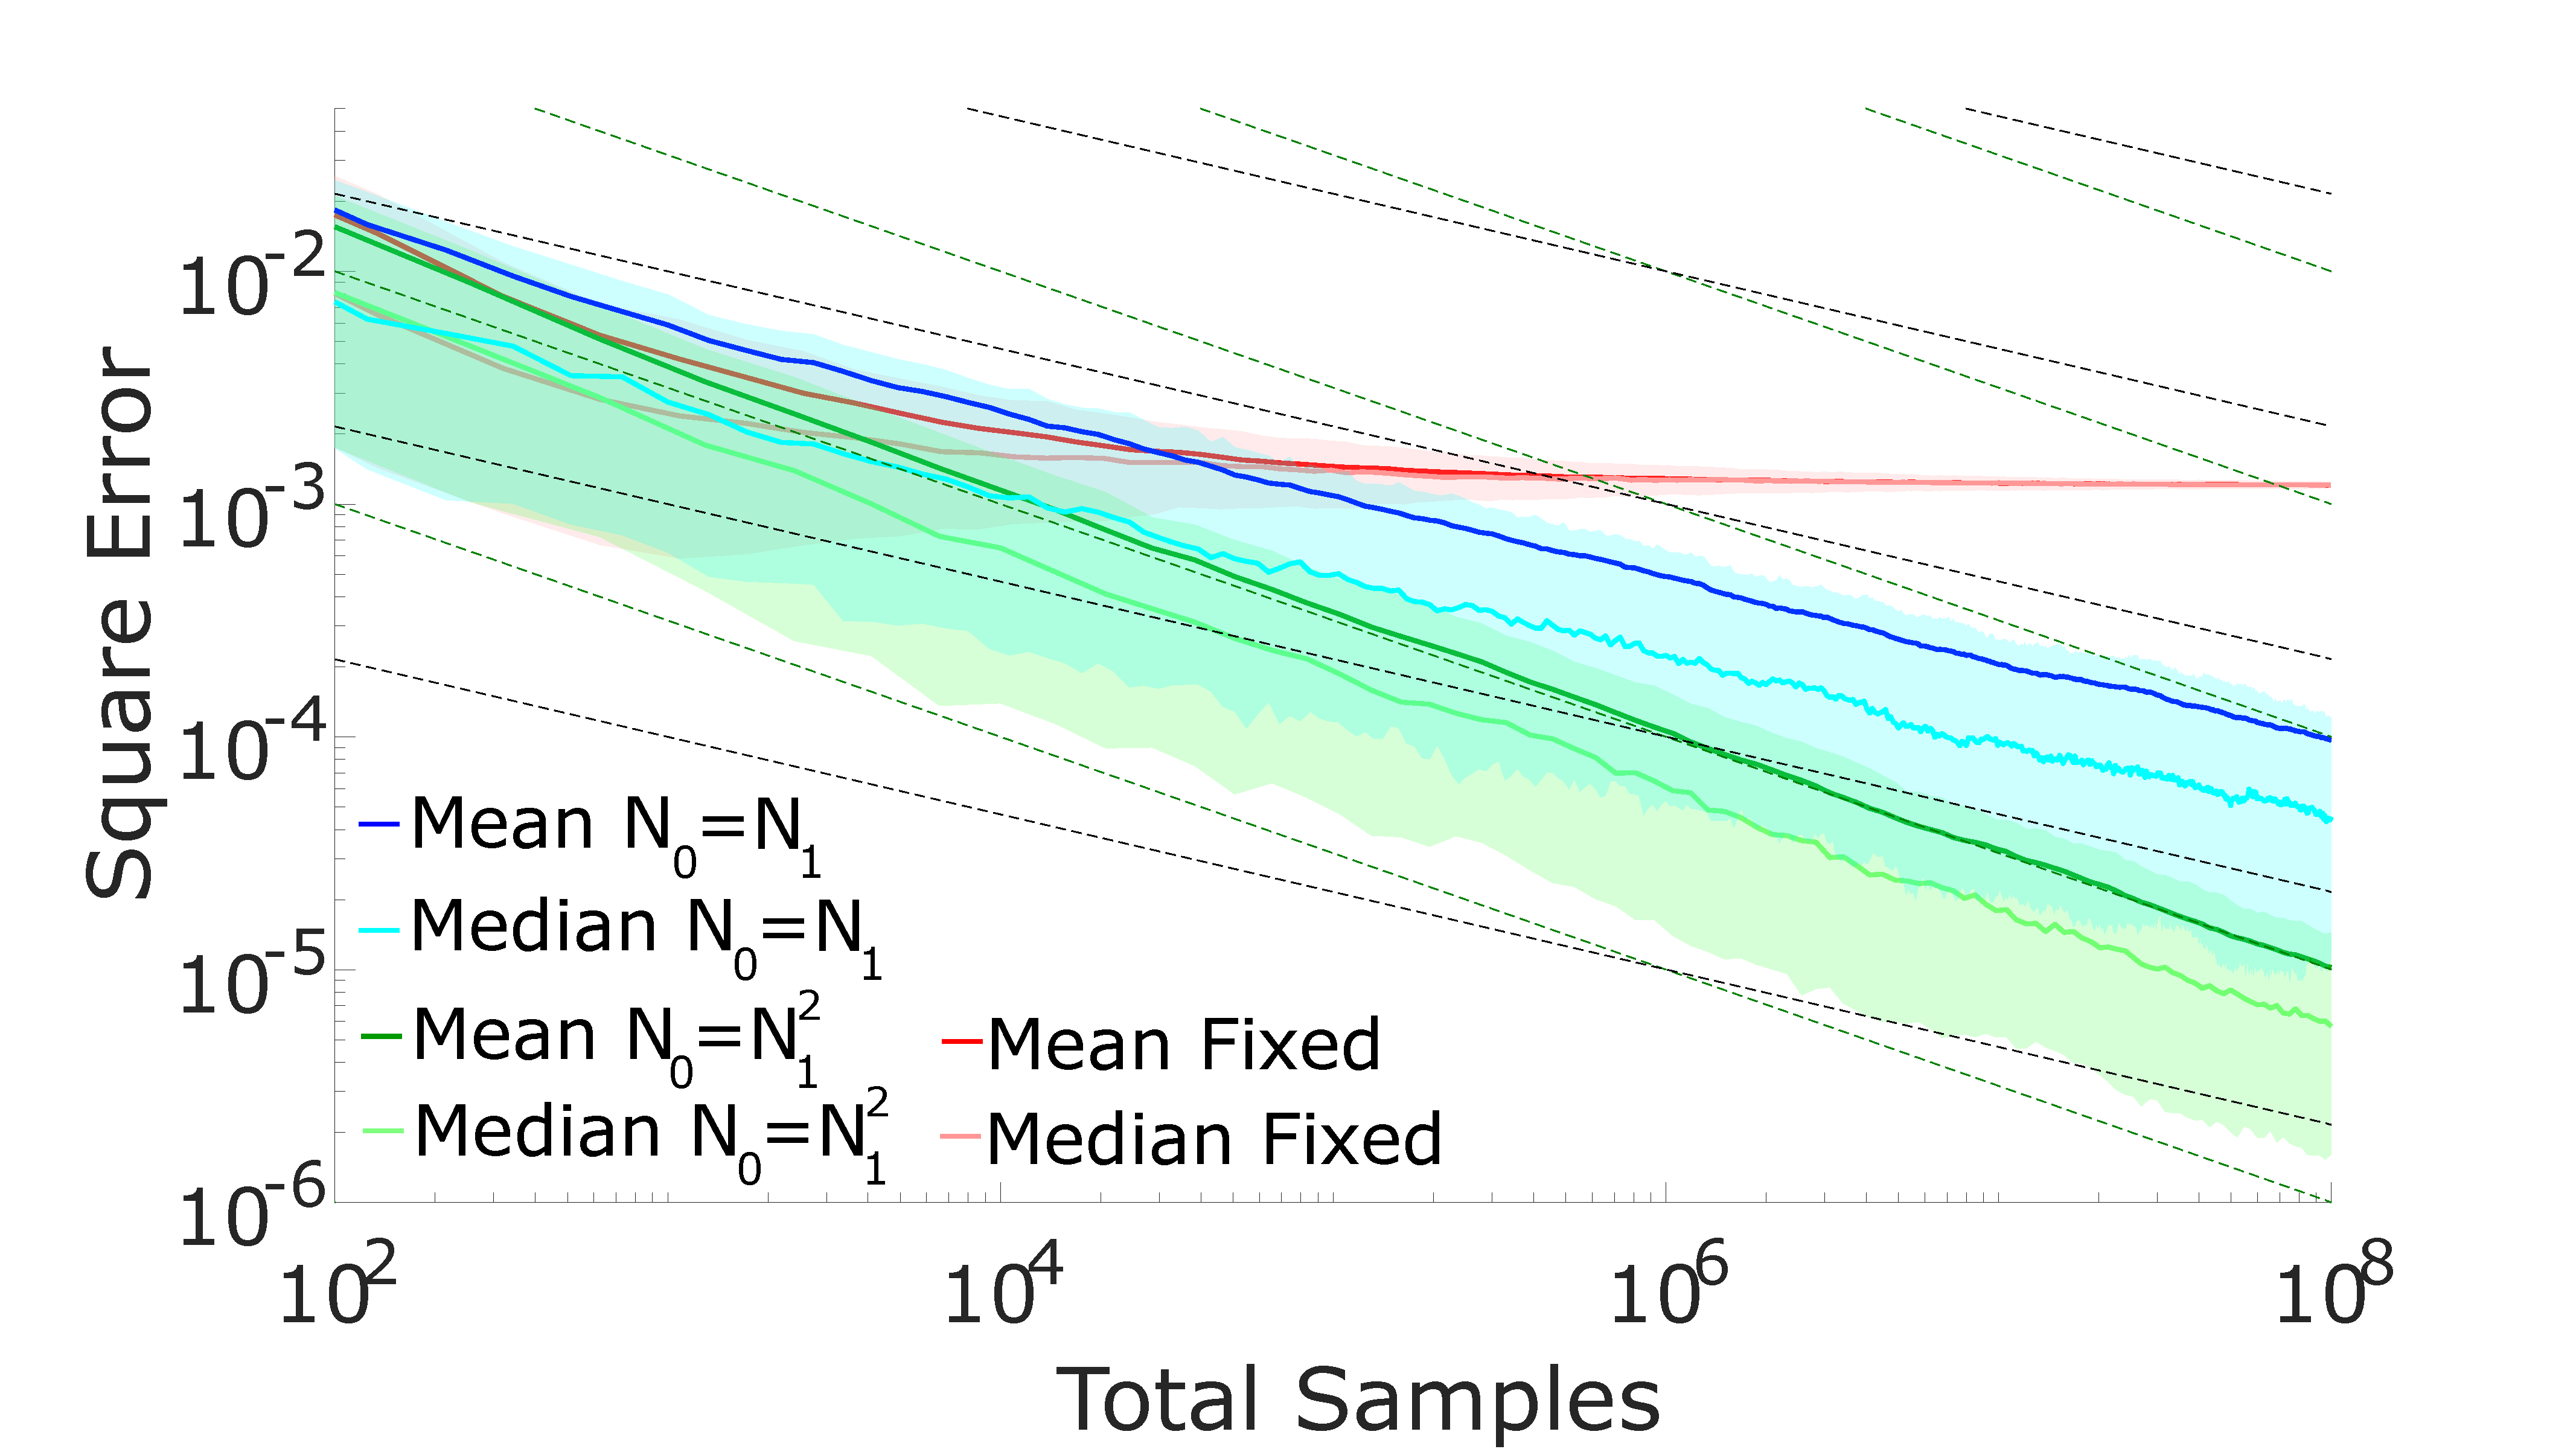
\includegraphics[width=0.5\textwidth,trim={1.5cm 0 3.5cm 0},clip]{repeat_nest_an}
	\caption{Empirical convergence of NMC to~\eqref{eq:repeat-nest} for an increasing total sample budget
		$T=N_0 N_1 N_2$.  Results are averaged over 1000 independent runs, while shaded regions give the 25\%-75\% quantiles.
		Shown in red is the convergence with a fixed $N_2=5$ and $N_1=N_2^2$, for which we see gives convergence
		to a biased solution, such that the error remains bounded as $T$ increases.  Shown in blue is the convergence
		when setting $N_0=N_1=N_2$, which we see converges at the expected $O(T^{-1/3})$ rate.  The black dashed lines
		provide a reference for this expected convergence of this estimator.  Shown in green is the convergence when
		setting $N_0=N_1^2=N_2^2$ which we seen again gives the theoretical convergence rate, this time $O(T^{-1/2})$
		with the dashed green lines providing reference.\label{fig:multi-nest}}
\end{figure}	

We next consider the empirical performance of different strategies for choosing $N_0, N_1$, $N_2$ under a 
finite fixed budget $T=N_0N_1N_2$.
To do this, we define $\alpha_1$ and $\alpha_2$ such that $N_0 = T^{\alpha_1}$, 
$N_1 = T^{\alpha_2(1-\alpha_1)}$, and $N_2 = T^{(1-\alpha_1)(1-\alpha_2)}$ and then consider the variation in the
mean squared error with $(\alpha_1,\alpha_2)$.  In particular, we look to establish the optimal empirical
setting under the fixed budget $T=10^6$.  To investigate how sensitive the empirically optimal 
allocation is to the problem at hand, we consider both the model described in~\eqref{eq:repeat-nest} and 
also two slight variations.  The first keeps everything the same as~\eqref{eq:repeat-nest} except the following replacements
\begin{subequations}
	\label{eq:repeat-nest2}
	\begin{align}
		y^{(0)} &\sim \mathrm{Uniform}(-1,1), \\
		f_2 \left(y^{(0:2)}\right)&=\exp\left(\frac{y^{(1)}+y^{(2)}-y^{(0)}}{2}\right)
	\end{align}
\end{subequations}
while the second instead replaces $y^{(0)}$ with $y^{(0)}/10$ in the definitions of $f_1$ and $f_2$.  The two
respectively have analytic solutions of $I=11/32$ and $I=39/160$.

To 
try and find the optimal $(\alpha_1,\alpha_2)$ and establish the variation of the MSE more generally,
we ran a Bayesian optimization
algorithm (specifically the ``Black-box Bayesian optimization'' algorithm of~\cite{rainforth2015workshopbopp}) to
optimize the mean squared error, estimated by averaging $1000$ trials at each iteration, with respect to 
$(\alpha_1,\alpha_2)$.  This produced the performance characterizations shown in
Figure~\ref{fig:multi-tau}, corresponding to contour plots of $\log_{10} \left(\E \left[(I_0-\gamma_0)^2\right]\right)$ as
estimated by the surrogate function generated after $200$ Bayesian optimization iterations.
It further found respective optimal values for $(\alpha_1,\alpha_2)$ of  $(0.53,0.36)$, $(0.55,0.69)$, and $(0.38,0.45)$,
giving corresponding values for $(N_0,N_1,N_2)$
of $(1563,10,64)$, $(1957,73,7)$, and $(192,47,111)$.\footnote{Note that there is inevitably a small bias introduced
	by the fact that each $N_k$ has to be a whole number.  The true values of $T$ used for these solutions
	were $1000320,\; 1000027,$ and $1001664$ respectively.}  By comparison, the asymptotically optimal
setup suggested by our theoretical results is $\alpha_1=\alpha_2=0.5$ giving $N_0=977$, $N_1=32$, and 
$N_2=32$.
This demonstrates that even for relatively large values of $T$, the finite budget optimal allocation can vary significantly
from the asymptotically optimal solution.  We also see that the relative optimally can change quite significantly with
changes to the target problem.  For example, the second modification meant it was more preferable to run less iterations of
the outer estimator, perhaps because it reduced the relative importance of $y^{(0)}$ compared to the other variables
in $f_1$ and $f_2$.  However, further work is required to
establish concrete empirical guidelines and investigate whether methods that adaptively allocate the number of
samples might be feasible.  In the meantime, the asymptotically optimal choice (presuming continuous differentiability) 
of $N_0 \propto N_1^2 \propto \dots \propto N_D^2$ seems to a reasonable practical choice on average.

\begin{figure}[t]
	\centering
	\begin{subfigure}[b]{0.32\textwidth}
		\centering
		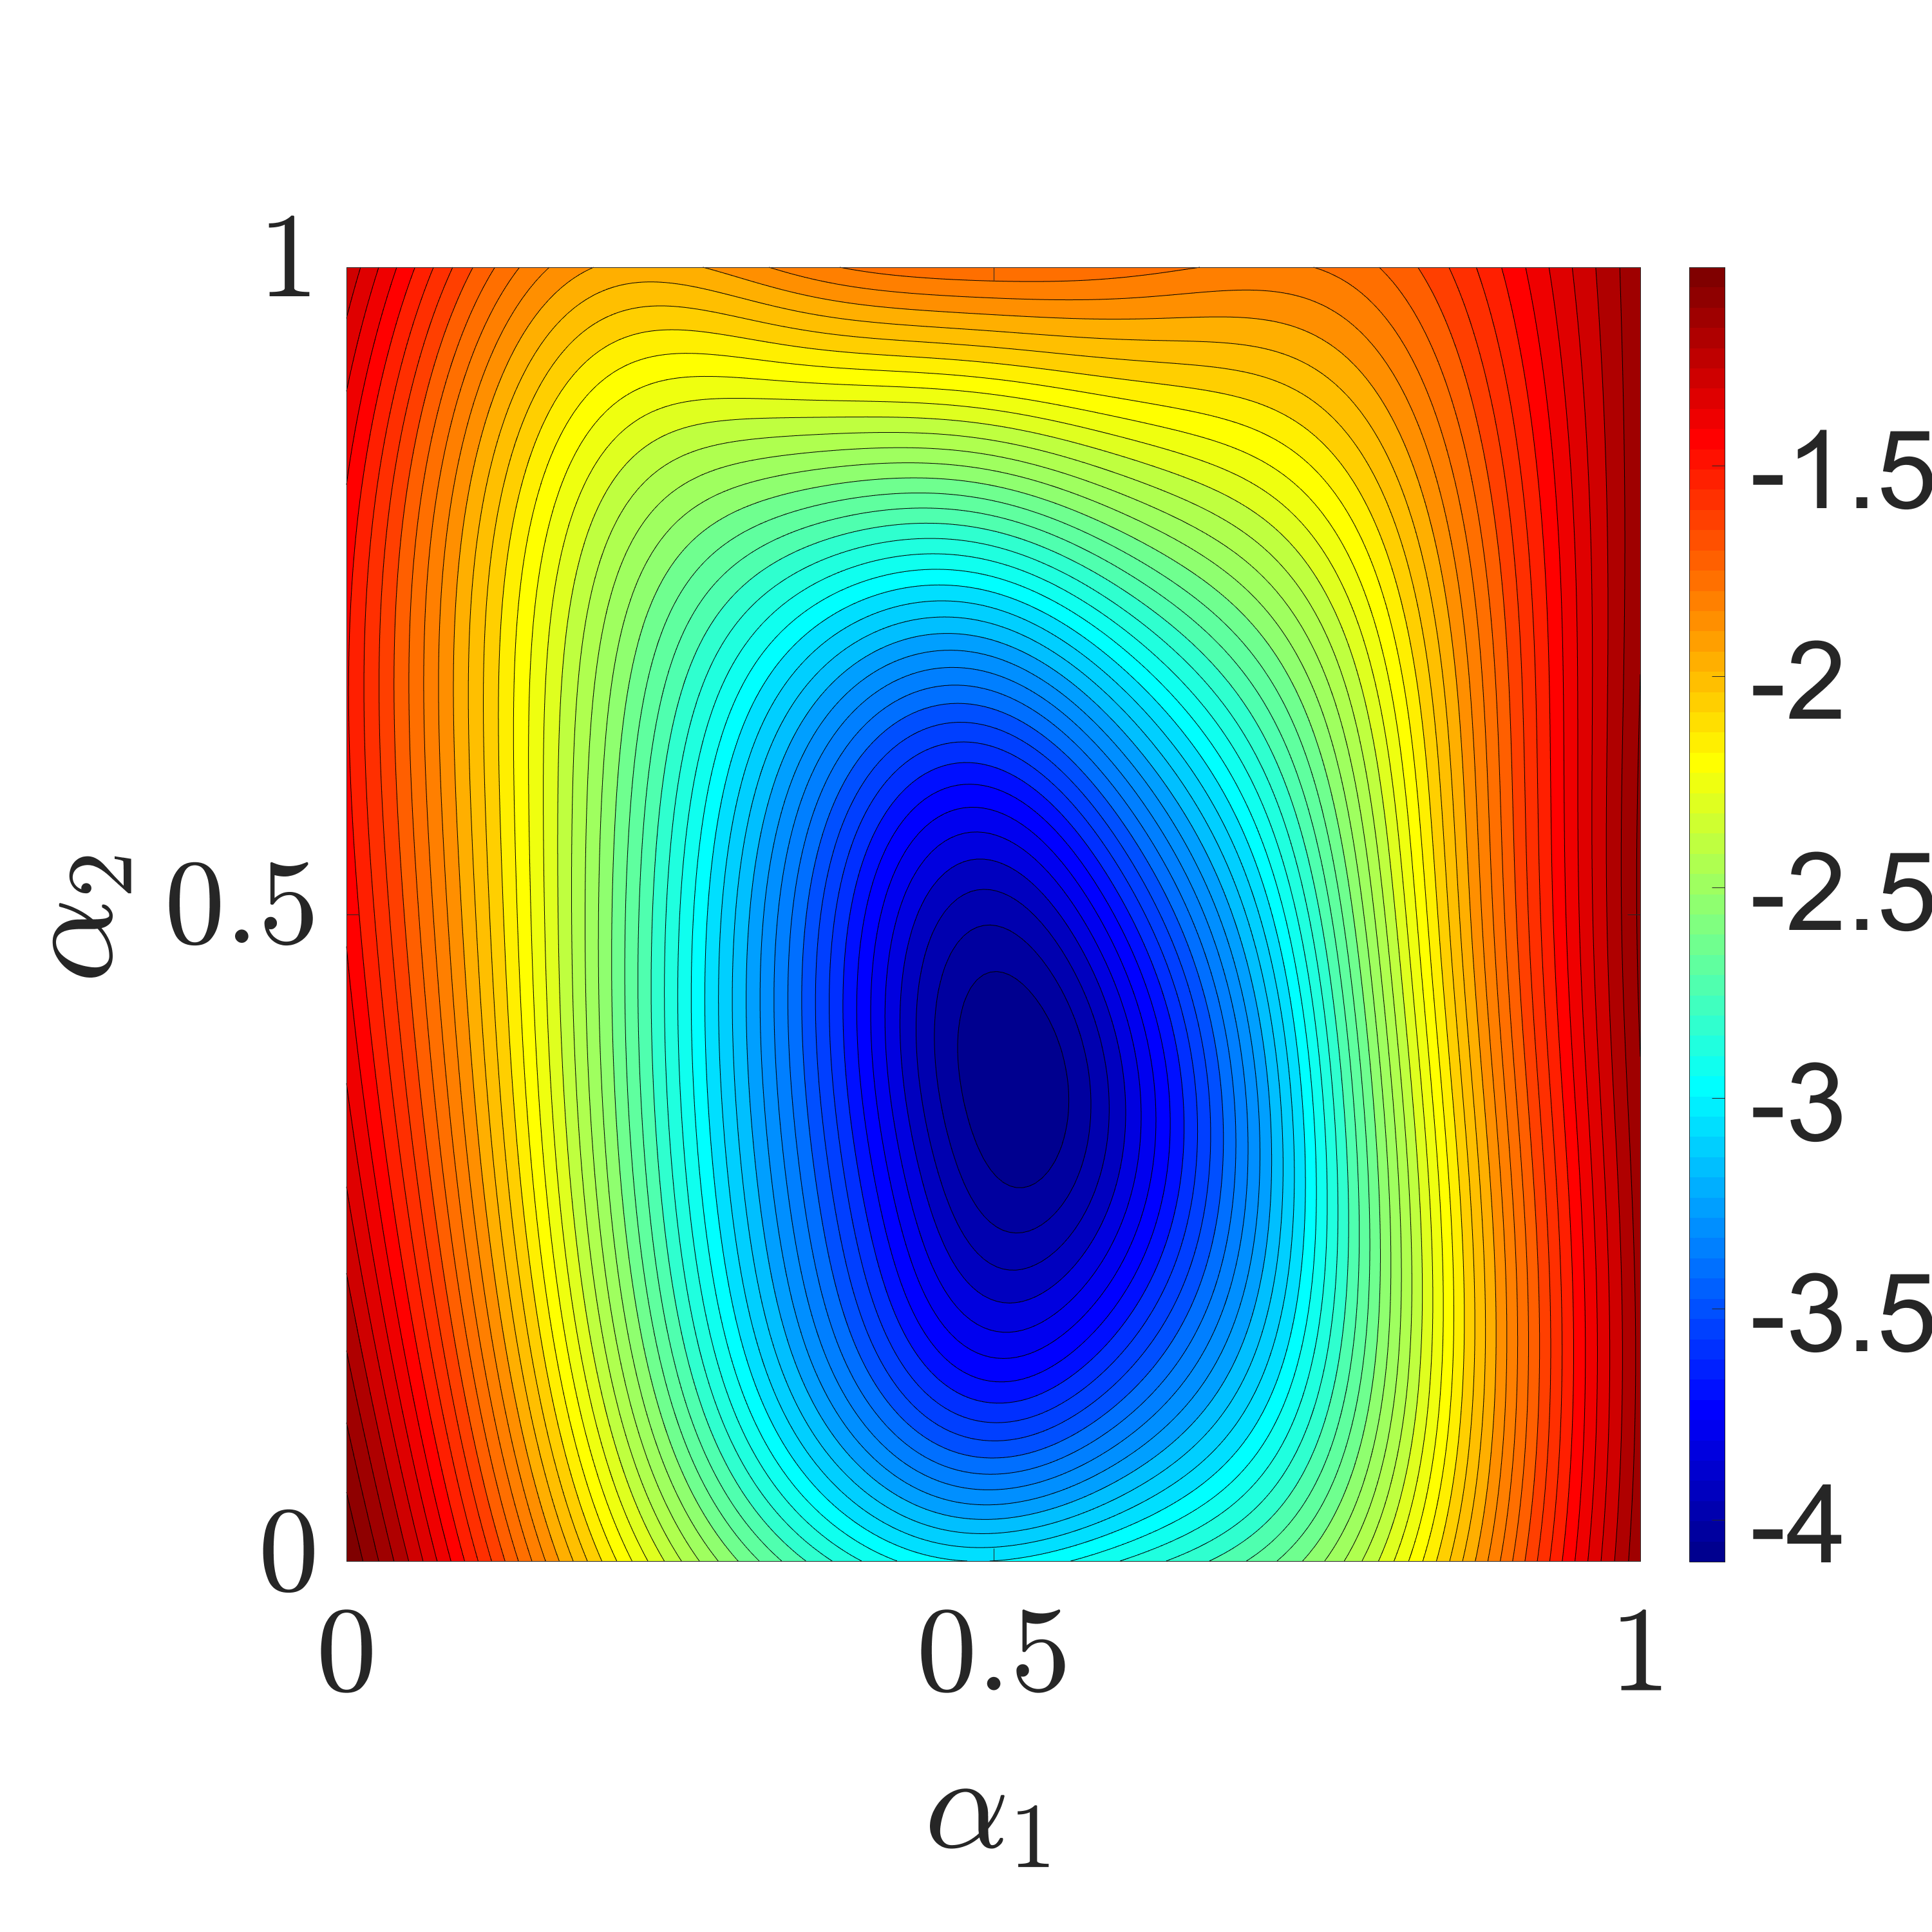
\includegraphics[height=0.88\textwidth]{tmax_1e6_model_3_contour_plot.pdf}
		\caption{Original}
	\end{subfigure}
	~\hspace{4pt}
	\begin{subfigure}[b]{0.32\textwidth}
		\centering
		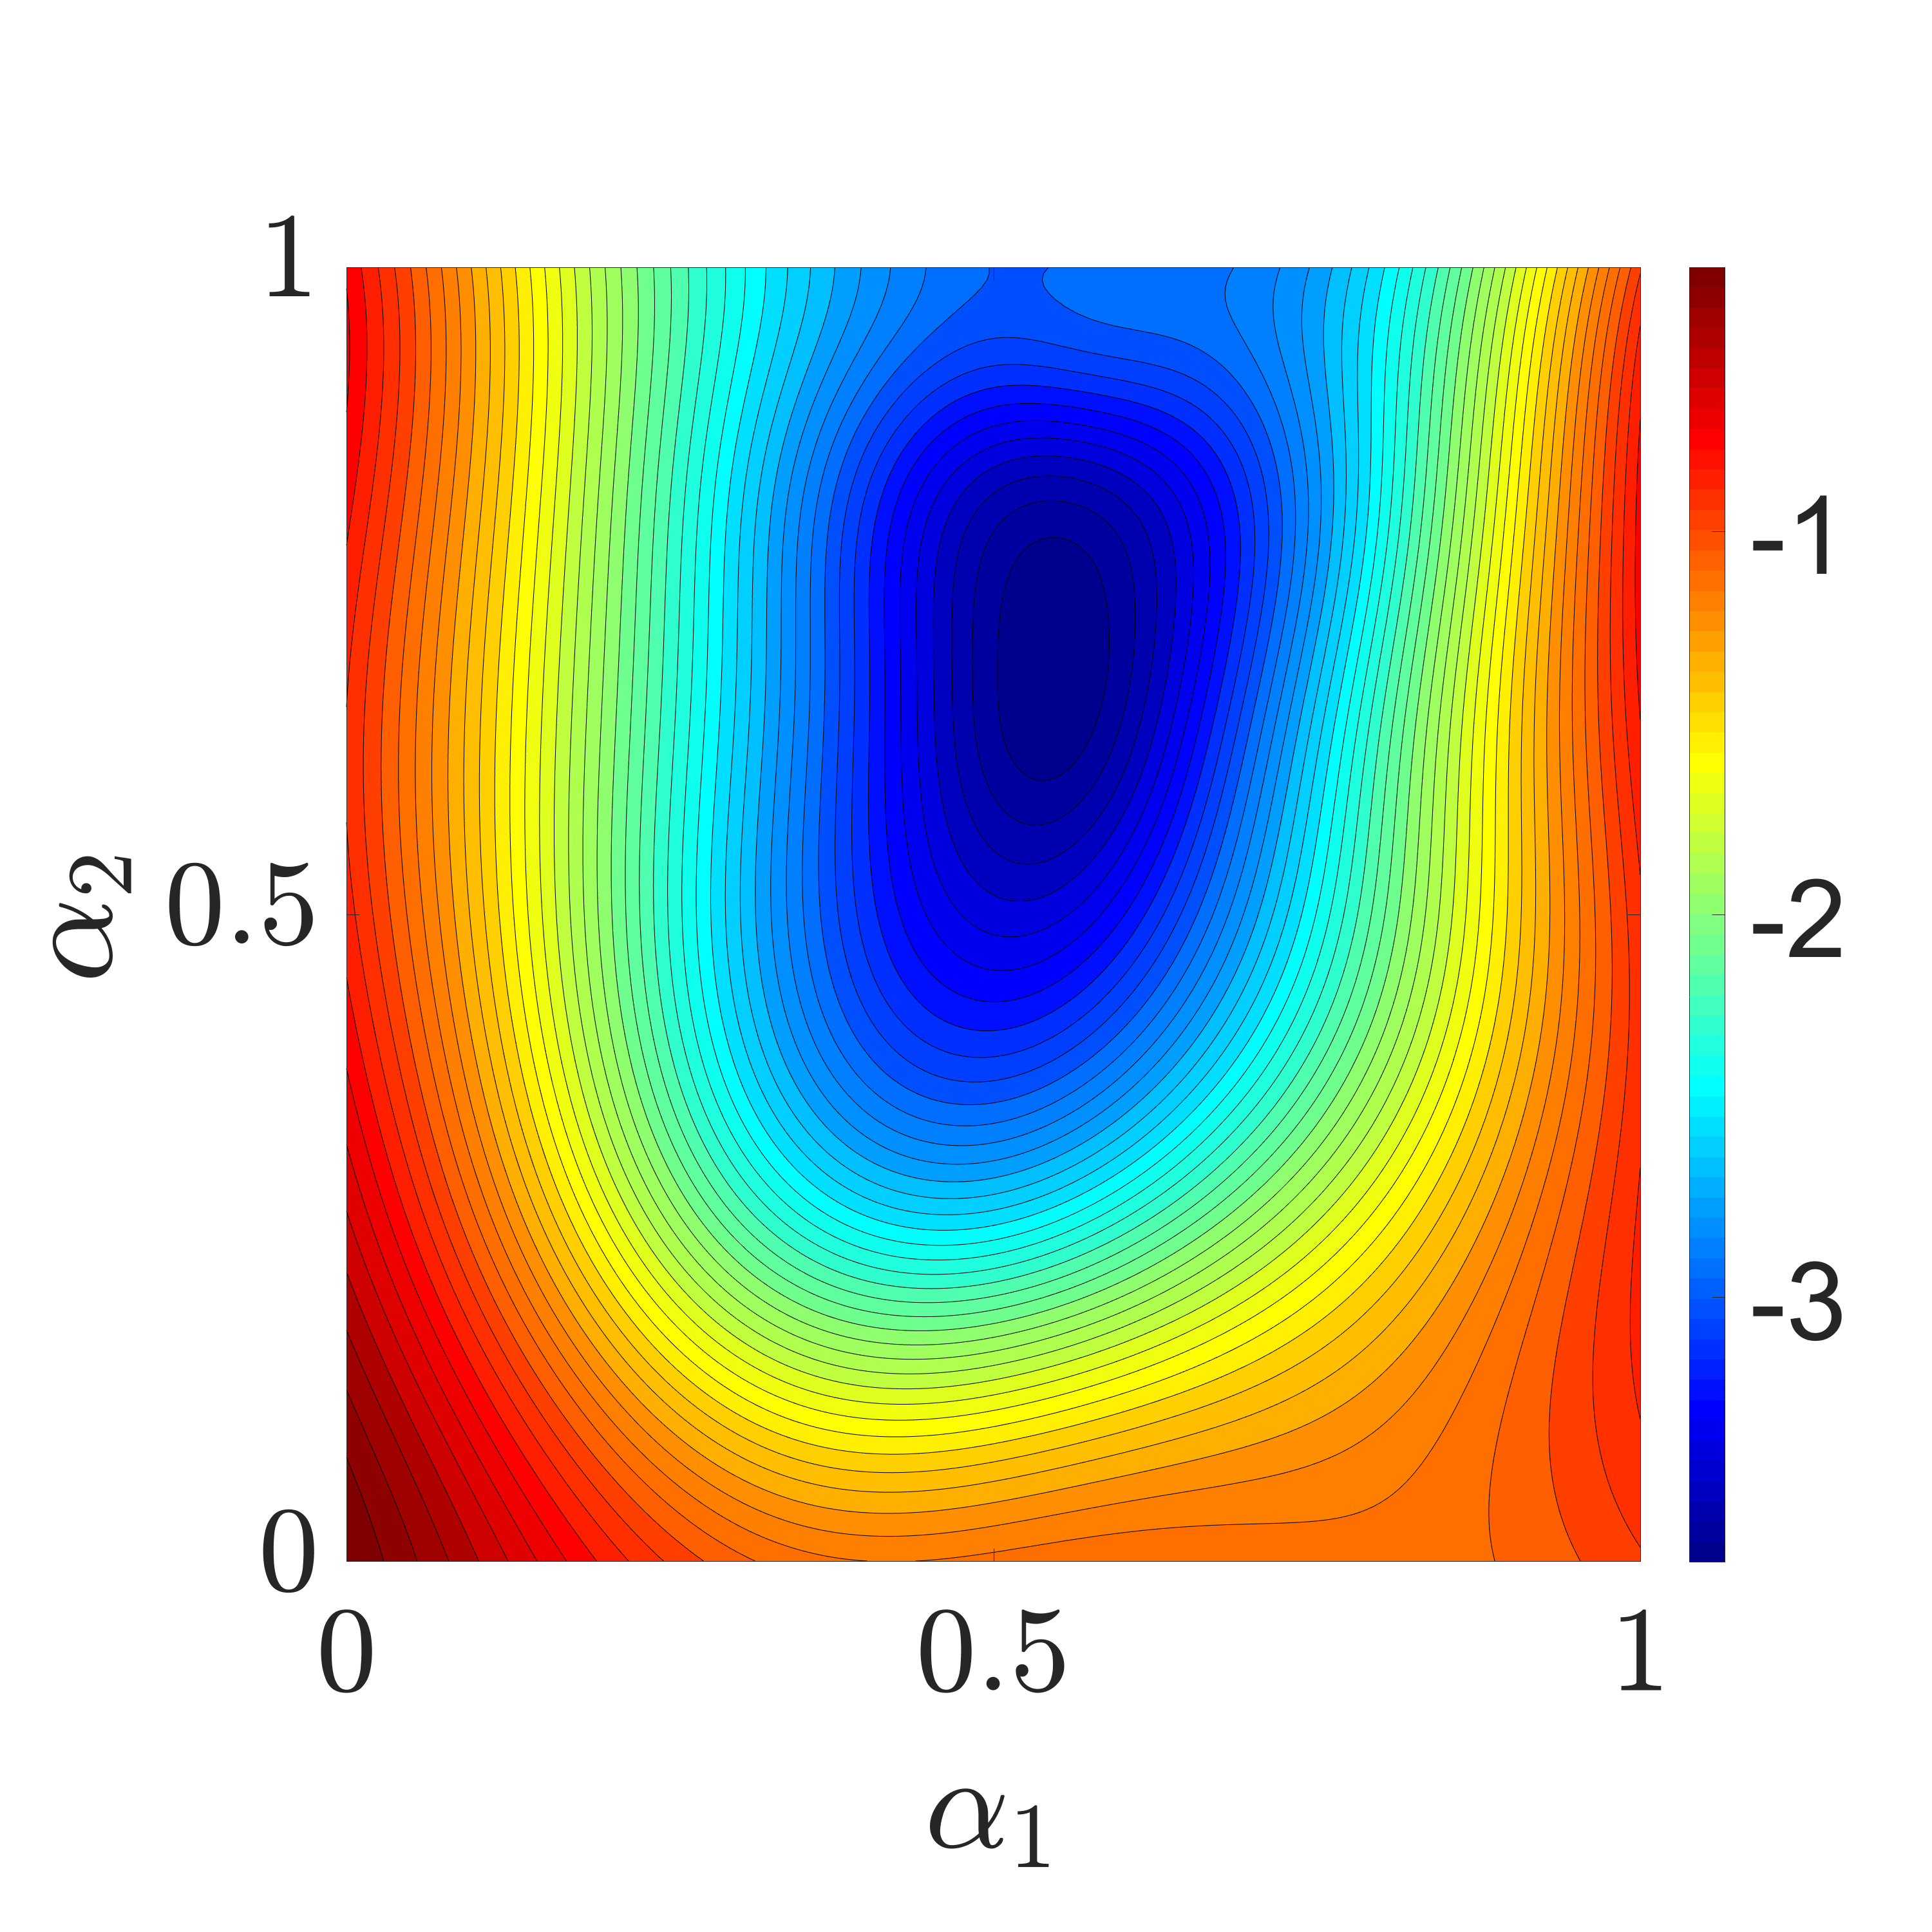
\includegraphics[height=0.88\textwidth]{tmax_1e6_model_2_contour_plot.pdf}
		\caption{First modification}
	\end{subfigure}
	~\hspace{-3pt}
	\begin{subfigure}[b]{0.32\textwidth}
		\centering
		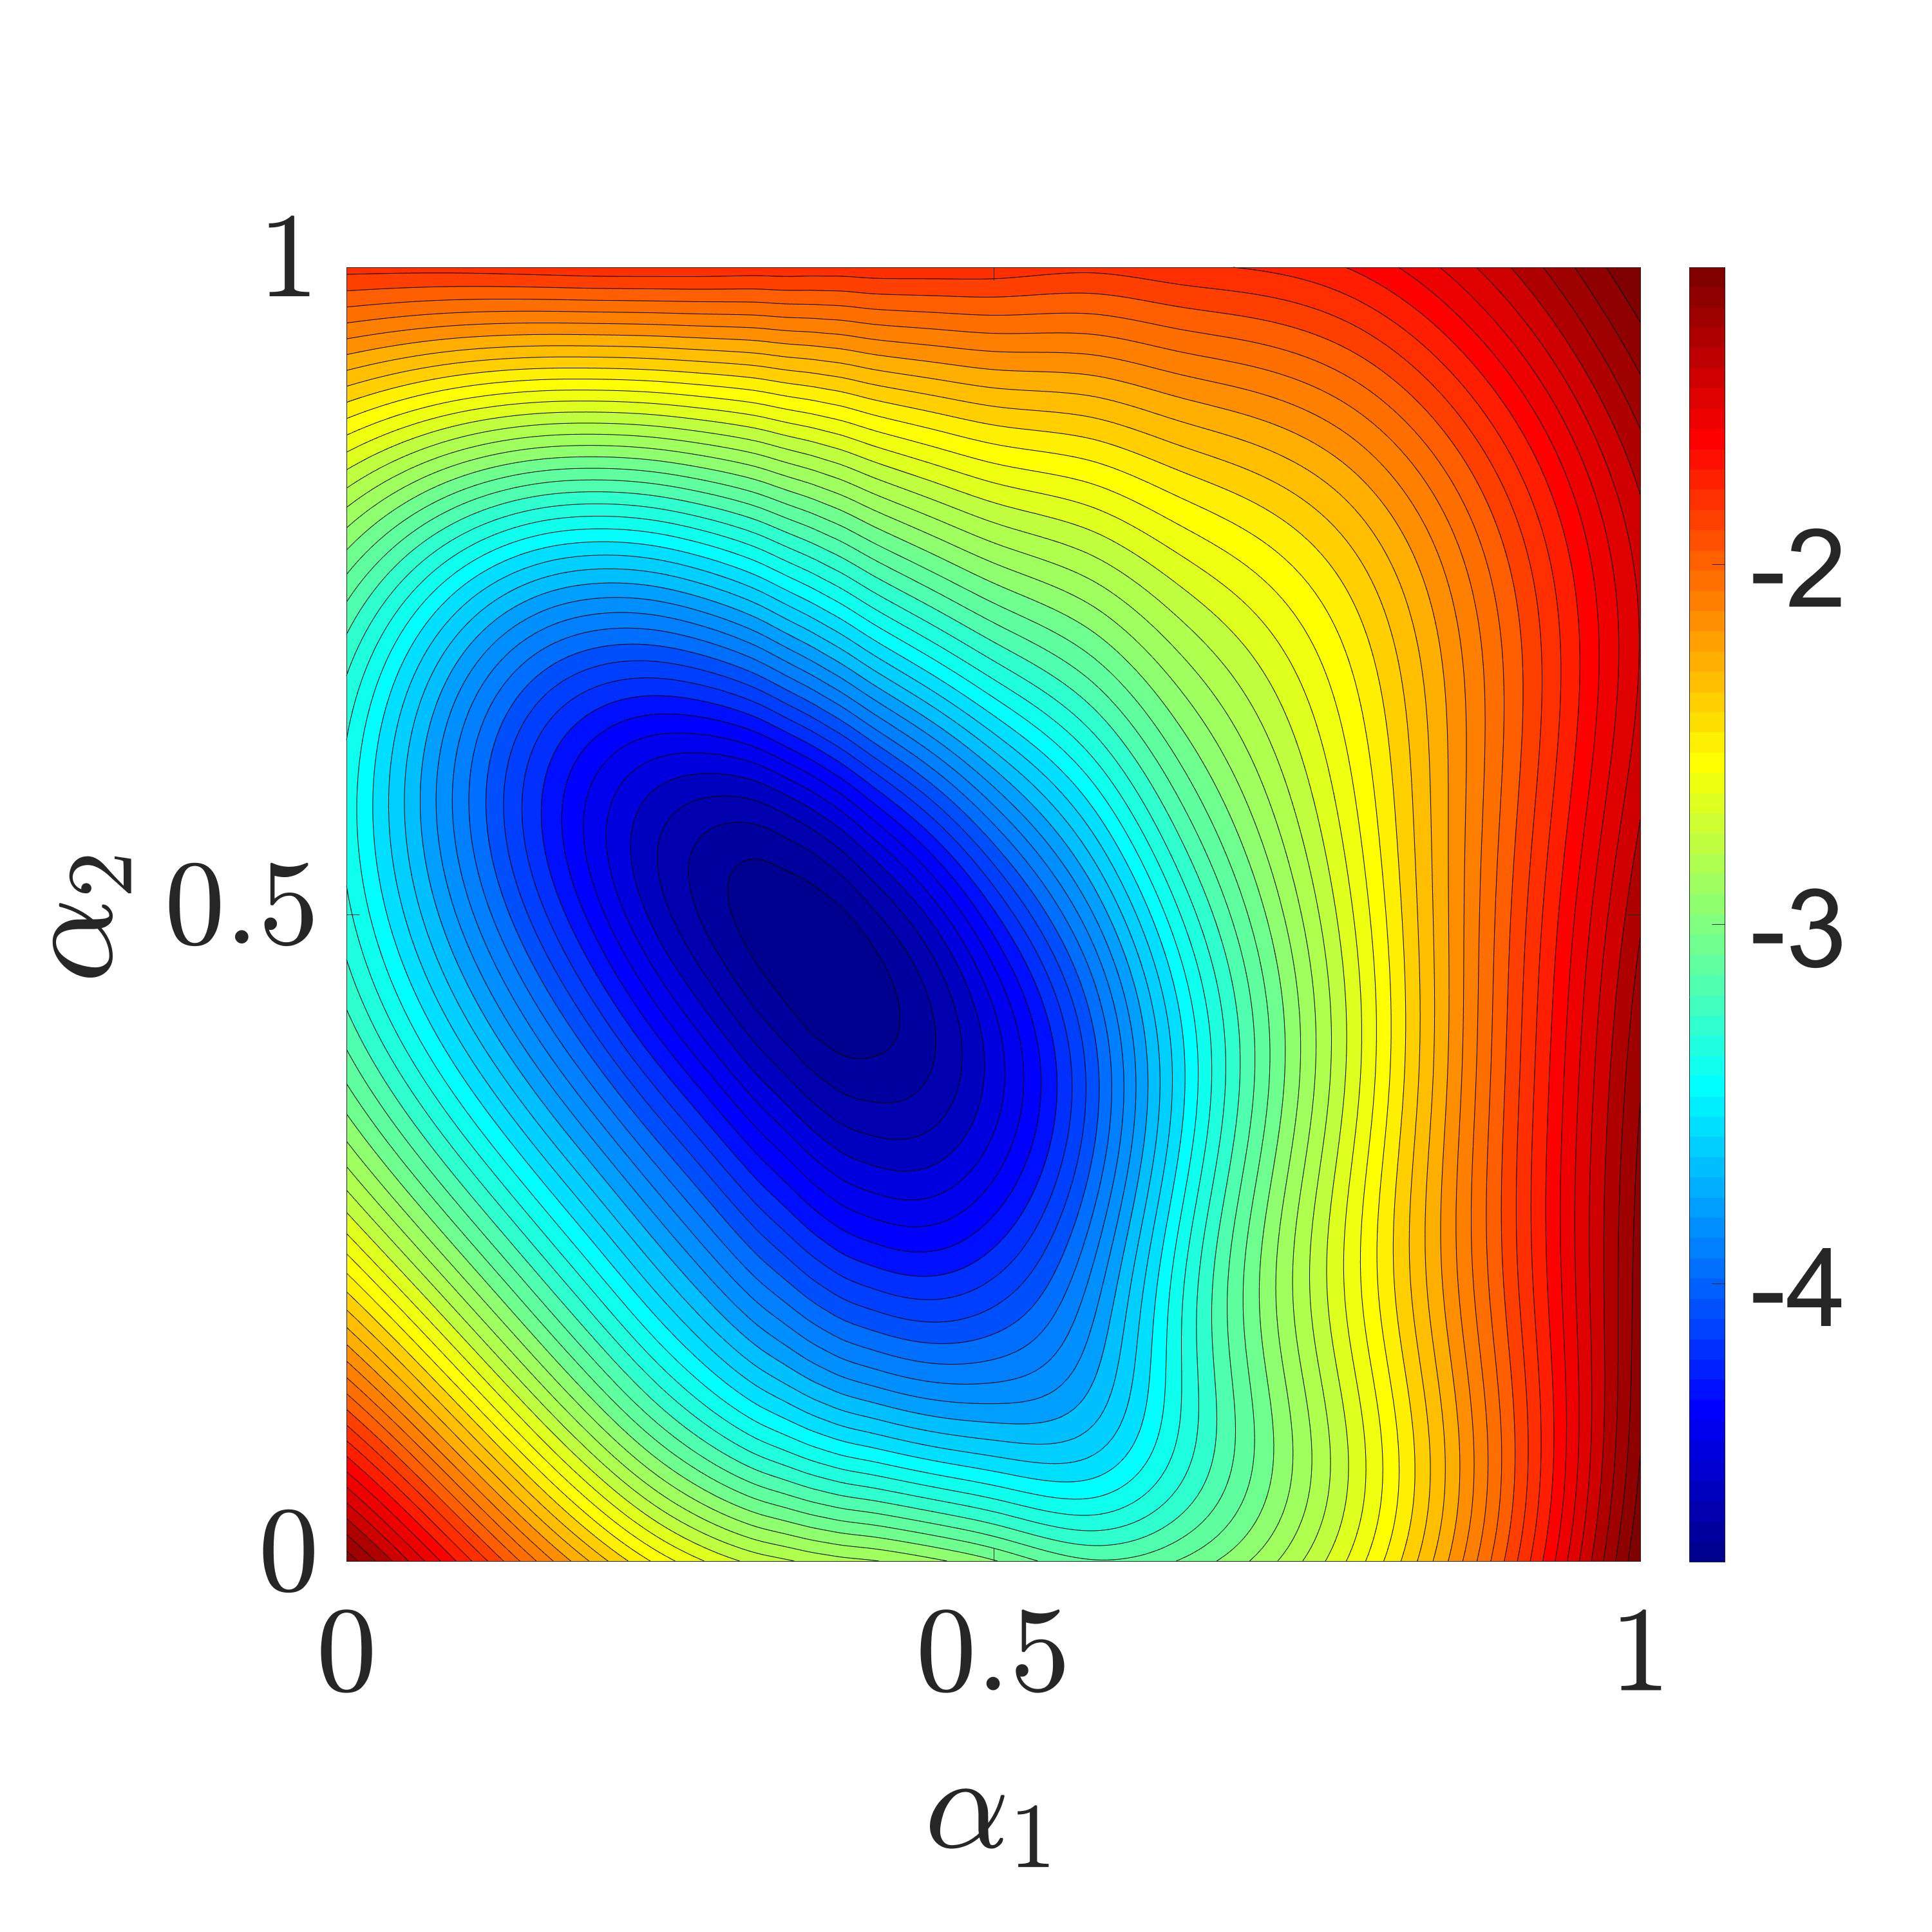
\includegraphics[height=0.88\textwidth]{tmax_1e6_model_4_contour_plot.pdf}
		\caption{Second modification}
	\end{subfigure}
	\caption{Contour plots of $\log_{10} \left(\E \left[(I_0-\gamma_0)^2\right]\right)$ (i.e. $\log_{10}$ MSE, estimated
		by averaging over $1000$ individual estimations)
		for different allocations of the sample budget $T=10^6$ between $N_0$, $N_1$,
		and $N_2$ for problem shown in~\eqref{eq:repeat-nest} and two modifications explained in
		the text.
		\label{fig:multi-tau}}
\end{figure}	
% !TEX root =  main.tex

\todo[inline]{Move these experimental section mostly into the main paper}

\section{Additional details pertaining to cancer simulator}
\label{sec:cancer_sim_app}

In this section we elucidate some more details about the cancer simulator described in the manuscript, provide more rigorous mathematical definitions for the relevant terms using the same nomenclature, and also include more results figures.

\subsection{Simulator details}
\label{sec:cancer_sim_details}

We define $I(T_{treat})$ to be the expected proportion of patients who receive treatment.
A particular patient is represented by $y\in\mathcal{R}^d$. Specifically, $y$ consists of only a single real number ($d=1$) representing the size of the tumour upon discovery. Initial tumour size is drawn from a scaled Rayleigh distribution.
The outcome of the simulator is then $\phi(y,z)\in\left\lbrace 0,1\right\rbrace $, and is the binary outcome of whether that particular patient and sample of unobserved parameters yield an expected tumour size below the threshold, $T_{opp}$, after a fixed time duration, $t_{max}$. The simulator is a pair of coupled, parameterized differential equations for the action of an anti-tumour treatment such as chemotherapy, as described in~\citet{enderling2014cancer}:
\begin{align}
&\frac{dc}{dt} = -\lambda c \log\big(\frac{c}{K}\big) - \xi c \\
&\frac{dK}{dt} = \phi c - \psi K c^{2/3},
\end{align}
where $c(t,x)\in\mathcal{R}_+$ represents tumour size, with initial size $y_n$.
Similarly, $K(t,x)\in\mathcal{R}_+$ represents the notion of a carrying capacity, with the initial carrying capacity, $K(0,z)$, set to a known constant $K_0$.
The magnitude of the patient response to an anti-tumour treatment (such as chemotherapy) is represented by $\xi\in[0,1]$, drawn from a beta distribution.
$\{\lambda, \psi, \phi\}\in\mathcal{R}_+^3$ represent the parameters of the simulator.
We also define $x _{n,m}= \{\lambda, \psi, \phi\, K_0, \xi\}$ and $z_{n,m}=\{x_{n,m}, T_{opp}, t_{max}\}$, where all but £$\xi$ are set to constant values. Expanding this to condition all values on $y_n$ is trivial given domain knowledge. Alternatively, they could also be drawn at random, but not be conditioned on $y_n$. Such relations are omitted here for simplicity.

We can now fully define $\phi$ as:
\begin{equation}
\phi(y_n,z_{n,m}) = \mathbbm{1}(c(t_{max}, x_{n,m})<T_{opp}).
\end{equation}
Taking the expectation of $\phi$ over $M$ different realisations of $z$ yields the estimate $(\hat{\gamma}_M)_n$. 
This value is the probability that treatment will be successful for a particular patient, marginalizing over possible unobserved dynamics. This is the point at which clinician decides whether initiate the treatment plan.
This decision is represented $f(y_n,(\hat{\gamma}_M)_n) \in [0,1]$ as:
\begin{equation}
f(y_n,(\hat{\gamma}_M)_n) = \mathbbm{1}((\hat{\gamma}_M)_n>T_{treat})
\end{equation}
where $T_{treat}$ is the minimum probability of success required for that patient to receive the treatment, and again, could be conditioned on $y$ also.
Taking the expectation of $f$ over patients yields the expected frequency with which the treatment will be delivered, given a value of $T_{treat}$. The hospital wishes to estimate the value $T_{treat}$ that maximizes the number of patients treated, while only treating those patients with the highest probability of success, and (in expectation) staying within the budgetary constraint.

\begin{figure}[t]
	\centering
	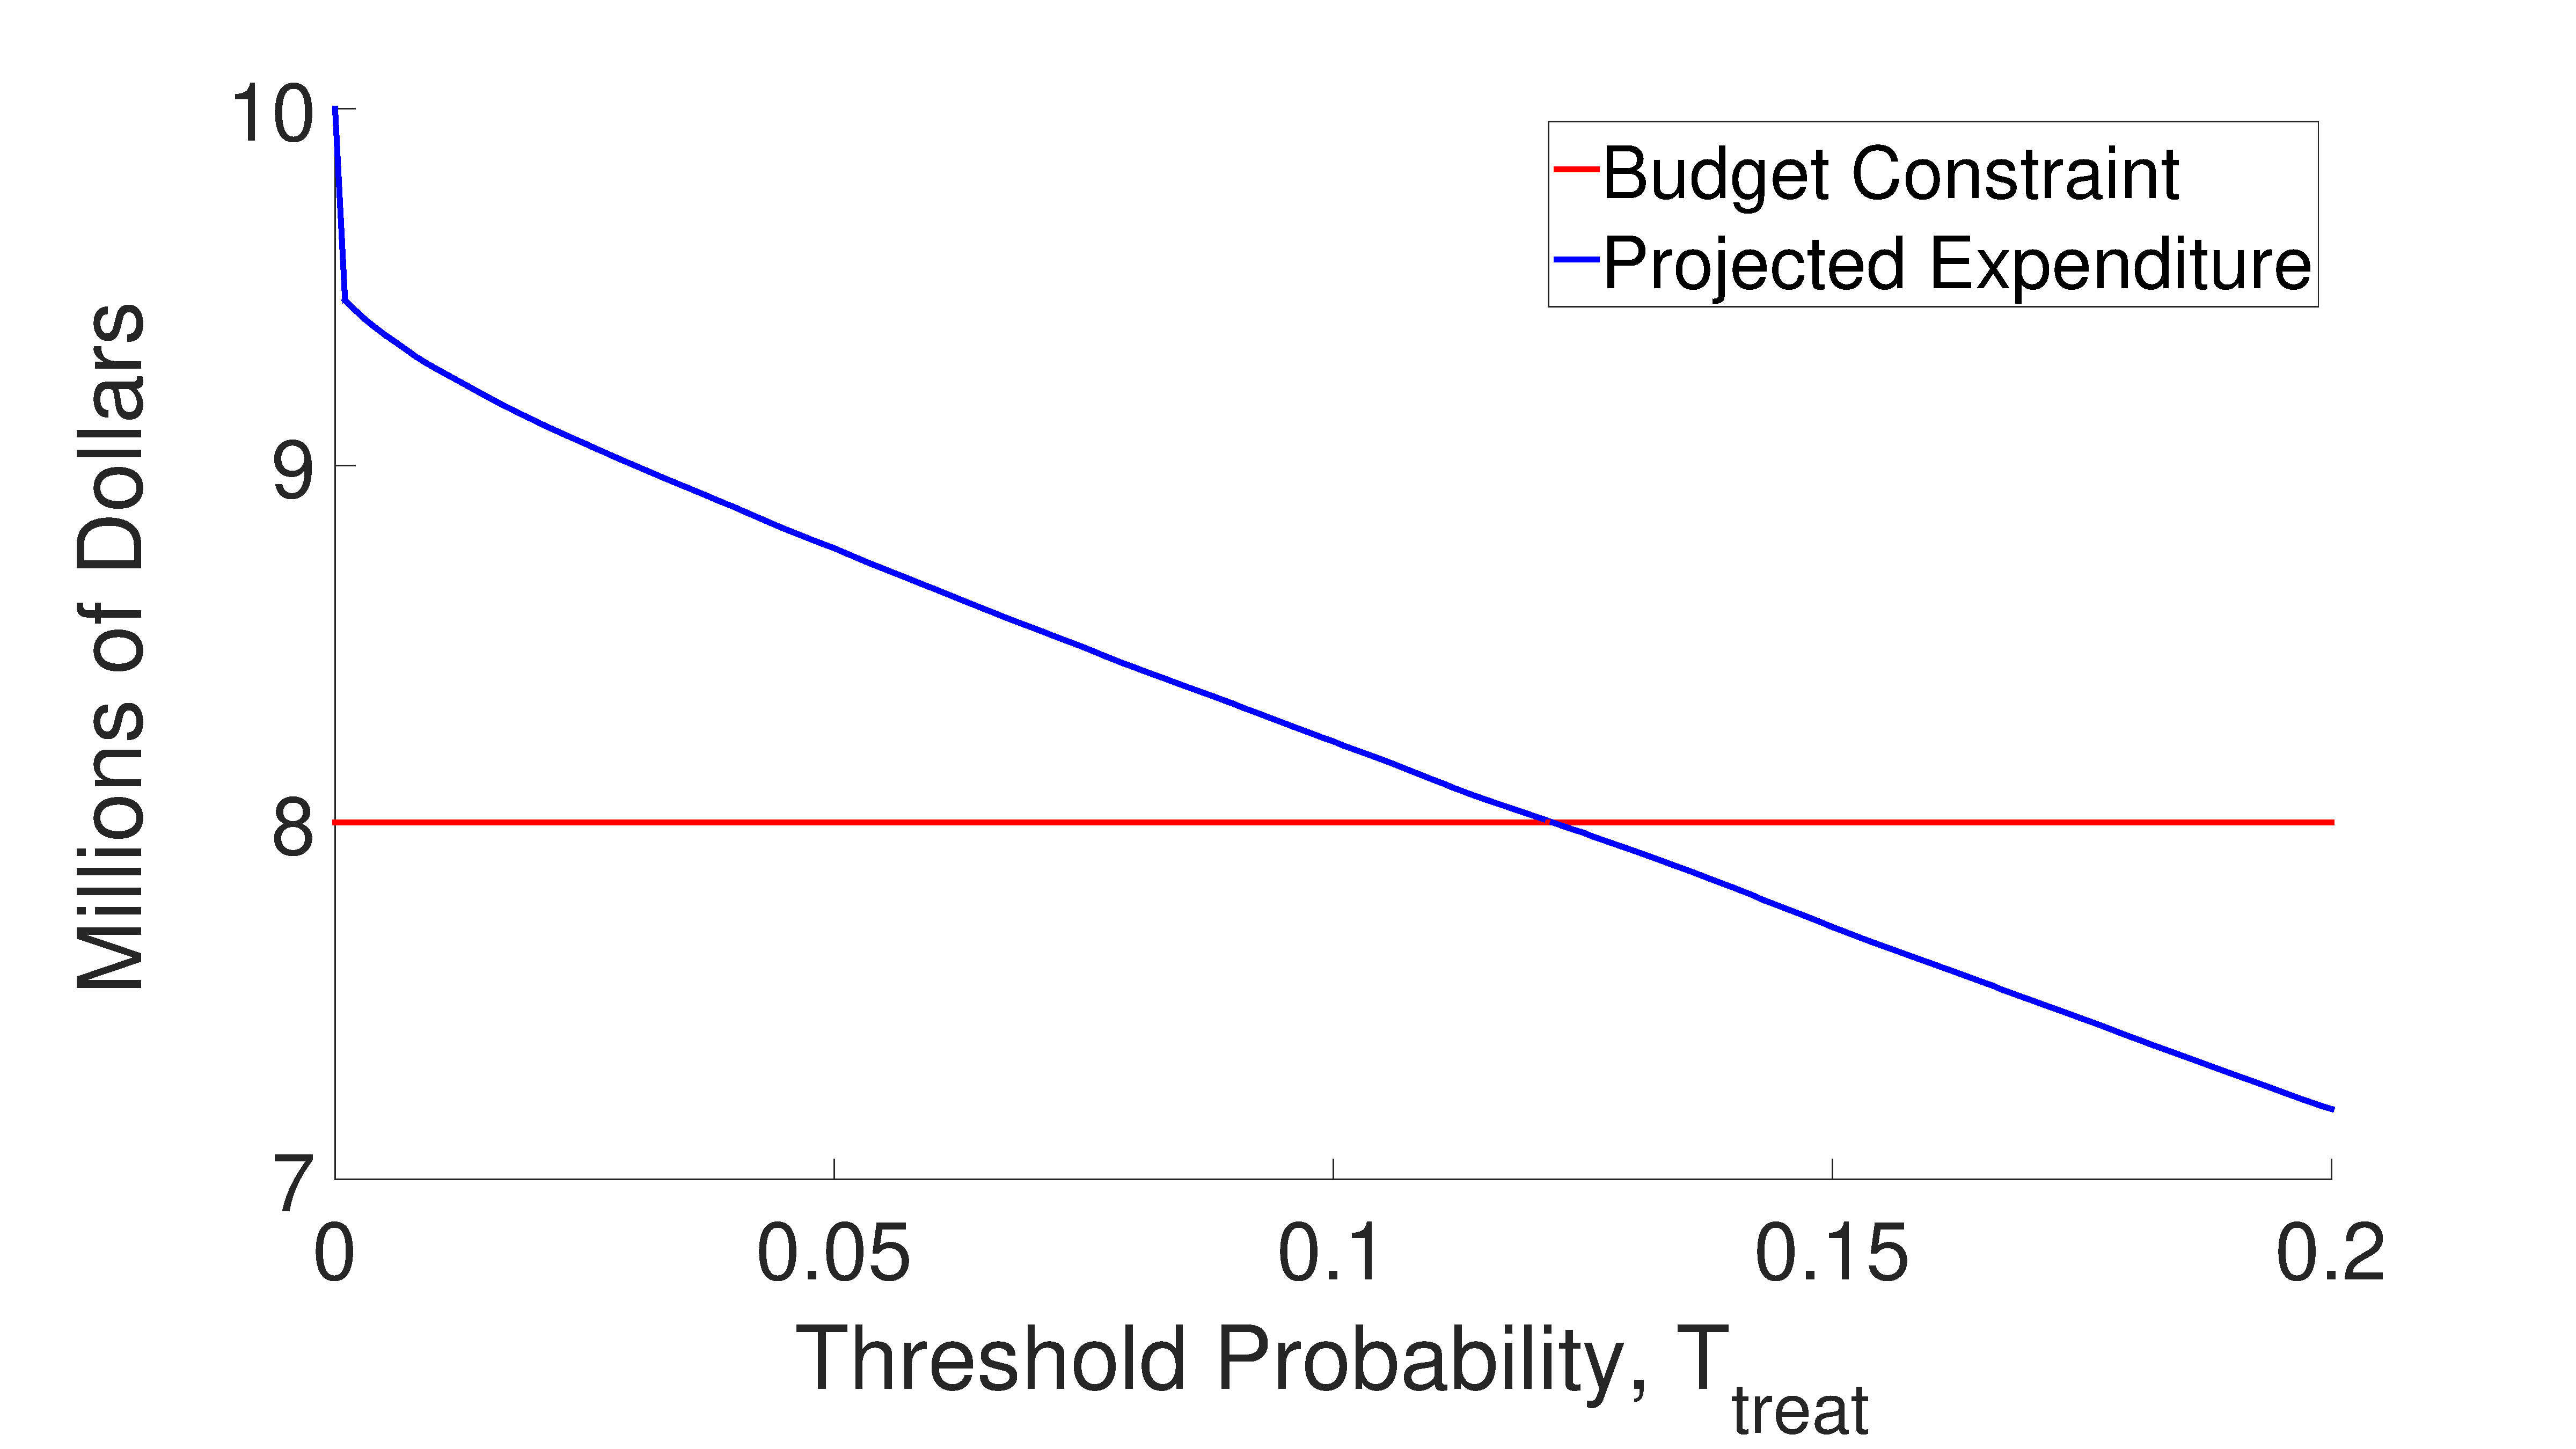
\includegraphics[width=0.48\textwidth]{budget}
	\caption{Projected expenditure (proportional to $I_{N,M}$) evaluated at different values of $T_{\mathrm{treat}}$. The budget constraint is shown by the horizontal red line. The optimal value of $T_{\mathrm{treat}}$ is found by the intersection 
		and occurs at $T_{\mathrm{treat}} = 12.5\%$. Evaluated was carried out at 100 $T_{\mathrm{treat}} \i$. Only the bottom 20\% is pictured as this is the operating range for most treatment centres. }
	\label{fig:emperical-cost}
\end{figure}

The model is completed by the definition of the following distributions and parameters.

\begin{align*}
& K_0 = 100000000, \quad
\phi = 0.001, \quad
\psi = 0.05, \quad
\lambda = 0.5, \quad
\xi \sim \text{Beta}(5, 2), \\
& c_0 \sim 1000*\text{Rayleigh}(10), \quad
T_{opp} = 2000,\quad
T_{treat} = 0.35, \quad
t_{max} = 250, \quad
t_{step} = 0.01 
\end{align*}

\subsection{Budget result}
\label{sec:cancer_sim_result}

In the example outlined above, the treatment centre is not actually attempting to evaluate the value of $I$, but to find the optimal value of $T_{treat}$ subject to a budgetary constraint. A simplistic way of evaluating the optimal value is to perform a dense search over different values of the parameter, each time evaluating the estimated expenditure, and select the best performing value.

Figure~\ref{fig:emperical-cost} shows the variation of predicted expenditure against the threshold probability, as well as the budget constraint. The intersection of these curves is the optimal setting of $T_{opp}$, here evaluated to be 12.5\%. From the blue line, it is clear that the relationship between expenditure and treatment probability is non-linear, especially at the extrema of the distribution, and hence the use of NMC was necessarily for evaluating the optimal value. 



